\documentclass{article}

\usepackage{url}
\usepackage[hmargin=1.5in]{geometry}
\usepackage{amsmath}
\usepackage{amssymb}
\usepackage{amsthm}
%\usepackage{eqnarray}
\usepackage{stmaryrd} %% needed for mapsto arrows in commutative diagrams
\usepackage{bm} %% for putting series names in bold
%%\usepackage{amsthm}
\usepackage{graphicx}
\usepackage{fancyhdr}
\usepackage{xparse}
\usepackage{enumitem}
%\usepackage{eqnarray}
%% colors
\usepackage[svgnames]{xcolor}
\let\Re\relax
\DeclareMathOperator{\Re}{Re}
\let\Im\relax
\DeclareMathOperator{\Im}{Im}

%% editing
\newcommand{\done}[1]{\textcolor{gray}{#1}}

\theoremstyle{definition}
\newtheorem{defn}{Definition}
%%\theoremstyle{plain}
%%\newtheorem{prop}{Proposition}

% convenience aliases
\newcommand{\maps}{\colon}
\newcommand{\acts}{\mathbin{\raisebox{\depth}{\rotatebox{-90}{$\circlearrowright$}}}}


% symbology
\newcommand{\Z}{\mathbb{Z}}
\newcommand{\R}{\mathbb{R}}
\newcommand{\C}{\mathbb{C}}
\newcommand{\Q}{\mathbb{Q}}
\usepackage{tikz}
\usepackage{tikz-cd}
\usepackage{rotating}
\newcommand*{\isoarrow}[1]{\arrow[#1,"\rotatebox{90}{\(\sim\)}"
]}

\newcommand{\series}[1]{\tilde{#1}}
\newcommand{\fracderiv}[3]{\partial^{#1}_{#2, #3}}
\newcommand{\holoL}[1]{\mathcal{H}L^{#1}} %% may no longer be needed
\newcommand{\blankbox}{{\fboxsep 0pt \colorbox{lightgray}{\phantom{$h$}}}}
\newcommand{\laplacepde}{\mathcal{D}}
\newcommand{\van}{\mathfrak{m}}
\DeclareMathOperator{\Ai}{Ai}
\usetikzlibrary{matrix,shapes,arrows,decorations.pathmorphing}
\tikzset{commutative diagrams/arrow style=math font}
\tikzset{commutative diagrams/.cd,
mysymbol/.style={start anchor=center,end anchor=center,draw=none}}
\newcommand\MySymb[2][\square]{%
  \arrow[mysymbol]{#2}[description]{#1}}
\tikzset{
shift up/.style={
to path={([yshift=#1]\tikztostart.east) -- ([yshift=#1]\tikztotarget.west) \tikztonodes}
}
}
\DeclareMathAlphabet{\mathpzc}{OT1}{pzc}{m}{it}

\newcommand*{\defeq}{\mathrel{\vcenter{\baselineskip0.5ex \lineskiplimit0pt
                     \hbox{\scriptsize.}\hbox{\scriptsize.}}}%
                     =}
\newcommand*{\defeqin}{\mathrel{\vcenter{\lineskiplimit0pt\baselineskip0.5ex
                     \hbox{\scriptsize.}\hbox{\scriptsize.}}}%
                     =}                     

%%\let\Re\relax
%%\DeclareMathOperator{\Re}{Re}

\newcommand{\laplace}{\mathcal{L}}
\newcommand{\borel}{\mathcal{B}}
\newcommand{\aexp}{\text{\ae}}
\newcommand{\deriv}[3]{\partial^{#1}_{#2 \text{ from } #3}}


\newtheorem{definition}{Definition}[section]
\newtheorem{prop}[definition]{Proposition}
\newtheorem{remark}[definition]{Remark}
\newtheorem{theorem}{Theorem}[section]
\newtheorem{corollary}[theorem]{Corollary}
\newtheorem{lemma}[definition]{Lemma}
%\newtheorem{conjecture}[definition]{Conjecture}
\newtheorem{claim}[definition]{Claim}
%\newtheorem{exercise}[definition]{Exercise}
\newtheorem*{notation*}{Notation}

\title{Borel regularity for ODEs and thimble integrals}
\author{Veronica Fantini and Aaron Fenyes}

\begin{document}
\maketitle

\section{Introduction}
\subsection{The unreasonable effectiveness of Borel summation}\label{intro:summation}
%%\subsection{A familiar process: Borel summation}\label{intro:summation}
You can often find a formal power series %\textcolor{magenta}{[double-check that this matches the $\tau$ from the position domain]}
\[ \series{\Phi} = \frac{c_0}{z^\tau} + \frac{c_1}{z^{\tau+1}} + \frac{c_2}{z^{\tau+2}} + \frac{c_3}{z^{\tau+3}} + \ldots, \]
with $\tau \in (0, 1]$, that looks or acts like a solution to a problem whose actual solutions are holomorphic functions of $z$. For example, if you want to understand how the solutions of the holomorphic ordinary differential equation (ODE)
\begin{equation}
\left[ \big[ \big(\tfrac{\partial}{\partial z}\big)^2 - 1 \big] + z^{-1} \tfrac{\partial}{\partial z} - \big(\tfrac{1}{3}\big)^2 z^{-2} \right] \Phi= 0. \label{eqn:bessel-rescaled-1}
\end{equation}
behave near $z = \infty$, you might start by looking for formal {\em transmonomial} solutions $e^{-\alpha z}\,\series{\Phi}$, where $\series{\Phi}$ is a formal power series of the kind above. Setting $\alpha = -\tfrac{1}{12}$ and $\tau = \tfrac{1}{2}$ gives a well-behaved recurrence relation for $\series{\Phi}$, which produces the solution \textcolor{magenta}{[check]}
\begin{equation}
e^{z/12} \left[ \frac{(-1)!!}{z^{1/2}} + \frac{5}{6} \cdot \frac{1!!}{z^{3/2}} + \frac{385}{216} \cdot \frac{3!!}{z^{5/2}} + \frac{17017}{3888} \cdot \frac{5!!}{z^{7/2}} + \ldots \right] \label{series:bessel-ex}
\end{equation}
and its constant multiples. As another example, you might rewrite the integral
\color{DodgerBlue}
\[ \Phi(z) = \int_{\Lambda} \exp\left[-\tfrac{1}{12} z \left(4u^3 - 3u\right)\right]\,du \]
\color{black}
\[ \Phi(z) = \int_{\Lambda} \exp\left[-z \left(\tfrac{1}{3} u^3 - \tfrac{1}{4} u\right)\right]\,du \]
as
% see expansion.sage
\[ e^{z/12} \int_{-\infty}^\infty e^{-z\tau^2/2} \left[ 1 - \frac{2}{3} \tau + \frac{5}{6} \tau^2 - \frac{32}{27} \tau^3 + \frac{385}{216} \tau^4 - \frac{224}{81} \tau^5 + \frac{17017}{3888} \tau^6 - \ldots \right] d\tau \]
using the substitution $\tfrac{1}{2} \tau^2 = \tfrac{1}{3} u^3 - \tfrac{1}{4} u + \tfrac{1}{12}$. Na\"{i}vely integrating term by term, you again get the transmonomial~\eqref{series:bessel-ex}.
\color{DodgerBlue}
\begin{align*}
& e^{z/12} z^{-1/2} \left[ (-1)!! + \frac{5}{6}\,1!!\,z^{-1} + \frac{385}{216}\,3!!\,z^{-2} + \ldots \right] \\
& = e^{z/12} z^{1/2} \left[ \frac{(-1)!!}{z} + \frac{5}{6} \cdot \frac{1!!}{z^2} + \frac{385}{216} \cdot \frac{3!!}{z^3} + \frac{17017}{3888} \cdot \frac{5!!}{z^4} + \ldots \right] \\
& = e^{z/12} \left[ \frac{(-1)!!}{z^{1/2}} + \frac{5}{6} \cdot \frac{1!!}{z^{3/2}} + \frac{385}{216} \cdot \frac{3!!}{z^{5/2}} + \frac{17017}{3888} \cdot \frac{5!!}{z^{7/2}} + \ldots \right]
\end{align*}
\color{black}

Once you have the formal solution $\series{\Phi}$, you might try to get an actual solution by applying {\em Borel summation}, which turns a formal power series into a function asymptotic to it. Borel summation works in three steps.
\begin{enumerate}
\item Thinking of $z$ as a ``frequency variable,'' we take the Borel transform (also known as formal inverse Laplace transform) of $\series{\Phi}$, producing a formal power series $\series{\phi}$ in a new ``position variable'' $\zeta$.
\item If $\series{\phi}$ has a positive radius of convergence we say $\series{\Phi}$ is {\em $1$-Gevrey}. We sum $\series{\phi}$ to get a holomorphic function $\hat{\phi}$ on a neighborhood of $\zeta = 0$. Then, by analytic continuation, we expand the domain of $\hat{\phi}$ to a Riemann surface $B$ with a distinguished 1-form $\lambda$---the continuation of $d\zeta$. \textcolor{orange}{[Nikita has a complementary picture where the Borel plane is the cotangent fiber? Ask more about this.]}
\item Furthermore, if $\hat{\phi}$ grows slowly enough along an infinite ray $b + e^{i\theta}[0, \infty)$ \textcolor{magenta}{[change, explain, or link to notation]} its Laplace transform $\laplace_b^\theta \hat{\phi}$ \textcolor{magenta}{[link to definition]} turns out to be a holomorphic function of $z$, well-defined on some sector of the frequency plane. In this case, we say $\tilde{\Phi}$ is {\em Borel-summable}, and we call $\hat{\Phi}:=\laplace_b^\theta \hat{\phi}$ its {\em Borel sum} at $b$. 
\end{enumerate}
The series $\series{\Phi}$ and its Borel sum $\hat{\Phi}$ have a special relationship, which is best described in the language of {\em Gevrey asymptoticity}. \textcolor{magenta}{[Do we need to extend these definitions, and the associated theorems, to cover slight series? Hopefully it wouldn't be too hard, but it would be a pain.]}
\begin{defn}
On an open sector $\Omega$ around $\infty$, a power series
\begin{equation}\label{series:asymp-defn}
\frac{a_1}{z} + \frac{a_2}{z^2} + \frac{a_3}{z^3} + \frac{a_4}{z^4} + \ldots
\end{equation}
is {\em asymptotic} to a holomorphic function $F$ if
\[ \left|F - \left(\frac{a_1}{z} + \frac{a_2}{z^2} + \ldots + \frac{a_{n-1}}{z^{n-1}} \right) \right| \in o_{z \to \infty}\big(|z|^{-n}\big) \]
over all orders $n$.

The {\em asymptotic expansion} map $\aexp^\theta$ sends a holomorphic function \textcolor{orange}{that vanishes at $\infty$ [if it vanishes at $\infty$ it sent to zero, so why this assumption?]} to the unique power series of the form \eqref{series:asymp-defn} which is asymptotic to it on the half-plane $\Re e^{i\theta}z > 0$ (see \cite[Theorem~C.11]{nikolaev2023existence}).
\end{defn}
\begin{defn}\label{def:unif-gevrey-asymp}
On an open sector $\Omega$ around $\infty$, a power series of the form \eqref{series:asymp-defn} is {\em uniformly $1$-Gevrey-asymptotic} to a holomorphic function $F$ if there's a constant $A \in (0, \infty)$ for which
\[ \left|F - \left(\frac{a_1}{z} + \frac{a_2}{z^2} + \ldots + \frac{a_{n-1}}{z^{n-1}} \right) \right| \lesssim \frac{A^n n!}{|z|^n} \]
over all orders $n$ and all $z \in \Omega$. We'll use $\lesssim$ throughout the paper to mean ``bounded by a constant multiple of,'' with the same constant over all the specified variables.
\end{defn}
To compare the Borel sum $\hat{\Phi}$ with the original series $\series{\Phi}$, let's take it one more step, sending it back into the world of formal power series by taking its asymptotic expansion.

\begin{enumerate}[start=4]
\item By construction, $\aexp^\theta \hat{\Phi} = \series{\Phi}$. It turns out that $\hat{\Phi}$ is not only asymptotic to $\series{\Phi}$, but {\em {uniformly} $1$-Gevrey}-asymptotic~\cite[Corollary~5.23]{diverg-resurg-i}.
\end{enumerate}

The Borel summation process is summarized in the following diagram:
\begin{center}
\begin{tikzcd}
& \text{problem} & \\
\hat{\Phi} \arrow[ru, dotted, no head, tail] \arrow[rr, mapsto, "\aexp^\theta", "\text{($1$-Gevrey)}"'] & & \series{\Phi} \arrow[lu, no head, tail, "\parbox{10mm}{\centering\scriptsize formally solves}"'] \arrow[dd, mapsto, "\borel"] \\
& & \\
\hat{\phi} \arrow[uu, mapsto, "\laplace_b^\theta"] & & \tilde{\phi} \arrow[ll, mapsto, "\text{sum}"] 
\end{tikzcd}
\end{center}

You can't be sure {\em a priori} that $\hat{\Phi}$ solves your original problem, even if you know that $\series{\Phi}$ is asymptotic to an actual solution. After all, $\series{\Phi}$ is asymptotic to lots of functions; Borel summation just picks one of them. In many cases, however, Borel summation picks correctly, delivering an actual solution to your problem. The question of how that happens is the starting point for this paper.

%\color{gray}
%\begin{itemize}
%\item \done{You can often find a formal power series $\tilde{\Phi} = \ldots$ that looks or acts like a solution to a problem whose actual solutions are holomorphic functions of $z$. For example\ldots}
%\begin{itemize}
%\item \done{Exponential integral: na\"{i}ve saddle point expansion.}
%\item \done{ODE: formal solution.} Existence theorem in \cite{diverg-resurg-iii}?
%\item Feynman diagram series?
%\end{itemize}
%\item Once you have $\tilde{\Phi}$, you might try applying {\em Borel summation}, which turns a formal power series into a function asymptotic to it.
%\begin{itemize}
%\item \done{Borel summation work in three steps. First we turn the formal power series $\tilde{\Phi}$ \textcolor{magenta}{[$\tilde{\Phi}(z)$]} in the ``frequency variable'' $z$ into a formal power series $\tilde{\phi}$ in a new ``position variable'' $\zeta$.}
%\item \done{The series $\tilde{\phi}$ turns out to have a \textcolor{magenta}{[finite]} positive radius of convergence, so it defines a holomorphic function $\hat{\phi}$. By analytic continuation, we can expand the domain of $\hat{\phi}$ to a Riemann surface $B$ with a distinguished 1-form $\lambda$---the continuation of $d\zeta$.}
%\item \done{If $\hat{\phi}$ grows slowly enough along an infinite ray $\Gamma_b^\theta := b + e^{i\theta}[0, \infty)$ \textcolor{magenta}{[decide notation]}, its Laplace transform $\laplace_b^\theta \hat{\phi} := \ldots$ is a holomorphic function of $z$, well-defined on some sector of the frequency plane. In this case, we say $\tilde{\Phi}$ is {\em Borel-summable}, and we call $\laplace_b^\theta \hat{\phi}$ its {\em Borel sum} at $b$.}
%\item {[Draw the square!]}
%\end{itemize}
%\item Different functions can be asymptotic to the same power series, and Borel summation picks one of them.
%\item In many cases, it picks correctly, producing an actual solution to your problem.
%\begin{itemize}
%\item The question of how that happens is the starting point for this paper.
%\item (In both of the cases that we study, the Borel sum of $\tilde{\Phi}$ is always taken at a zero of $\lambda$, rather than an arbitrary point in $B$. For ODEs, our treatment explains why the zeroes of $\lambda$ play a special role.)
%\end{itemize}
%\end{itemize}
%\color{black}
\subsection{A new perspective: Borel regularity}
\subsubsection{Introducing Borel regularity}
\begin{itemize}
\item Start instead with a holomorphic solution $\Phi$.
\item Taking its asymptotic expansion along the half-plane $\Re e^{i\theta}z > 0$, we get a formal power series $\series{\Phi}$.
\end{itemize}
%\textcolor{Tan}{We consider a new diagram: we start reading it from the upper-left corner, namely we assume there exists a holomorphic function $\Phi$ which is asymptotic to a formal power series $\series{\Phi}$ as $\Re e^{i\theta}z$ goes to $\infty$ in the direction of $\theta$}

\begin{center}
\begin{tikzcd}
& \text{problem} & \\
\Phi \arrow[ru, no head, tail, swap, "\text{solves}"' ] \arrow[rrd, mapsto, "\aexp^{\theta}"]& & \\
\hat{\Phi} \arrow[rr, "\aexp^{\theta}", "\text{($1$-Gevrey)}"'] & & \series{\Phi} \arrow[luu, no head, tail, swap, "\parbox{10mm}{\centering\scriptsize formally solves}"] \arrow[dd, mapsto, "\borel"] \\
& & \\
\hat{\phi} \arrow[uu, mapsto, "\laplace_b^\theta"] & & \series{\phi} \arrow[ll, mapsto, "\text{sum}"] 
\end{tikzcd}
\end{center}
If $\series{\Phi}$ is Borel-summable, as described in Section~\ref{intro:summation}, its Borel sum $\hat{\Phi}$ is a new holomorphic function.
Since different functions can be asymptotic to the same power series, taking the Borel sum of the asymptotic series of $\Phi$ must smooth away some details. We'll therefore call this process {\em Borel regularization}. Explicitly, Borel regularization works in four steps.
\begin{enumerate}
\item Take the asymptotic expansion $\series{\Phi} = \aexp^{-\theta} \Phi$.
\item Take the Borel transform $\series{\phi} = \borel \series{\Phi}$.
\item Take the sum $\hat{\phi}$ of $\series{\phi}$, and expand its domain to a Riemann surface with a distinguished $1$-form, as before. This is possible, by definition, if $\series{\Phi}$ is $1$-Gevrey.
\item Take the Laplace transform $\hat{\Phi} = \laplace_{\zeta, 0}^\theta \hat{\phi}$. This is possible, by definition, if $\series{\Phi}$ is Borel-summable. \textbf{[Should we be allowed to take the Laplace transform at another points $b \in B$ instead?]}
\end{enumerate}
We'll say a function is {\em Borel-regularizable} if its asymptotic expansion is Borel-summable, ensuring that we can carry out the last two steps.

Defining a regularization process picks out a class of regular functions: the ones that are invariant under regularization. We'll say a function is {\em Borel regular} if it's Borel-regularizable and Borel regularization leaves it unchanged. In other words, $\Phi$ is Borel regular if $\hat{\Phi} = \Phi$.
\subsubsection{Borel regularity as a good approximation condition}
Borel regular functions can be characterized as functions that are approximated well, asymptotically, by polynomials. Watson showed a century ago \cite{watson} that a function $F$ that vanishes at $\infty$ is Borel regular whenever its asymptotic expansion is uniformly $1$-Gevrey-asymptotic to it on an obtuse-angled sector around $\infty$ (see Definition~\ref{def:unif-gevrey-asymp}).

Watson's theorem was soon improved by Nevanlinna \cite{nevanlinna} (see a modern proof in \cite{nikolaev2023exact} Theorem~B.15 and a generalization to power series with fractional power exponents in \cite{delabaere--rosoamanana}), and improved again later by Sokal \cite{sokal1980improvement}. These improvements tell us that the obtuse-angled sector around $\infty$ in the statement above can be replaced with an open disk whose boundary touches $\infty$---that is, an open half-plane which doesn't contain $0$, and may be displaced from $0$ by some distance $c$.
\begin{center}
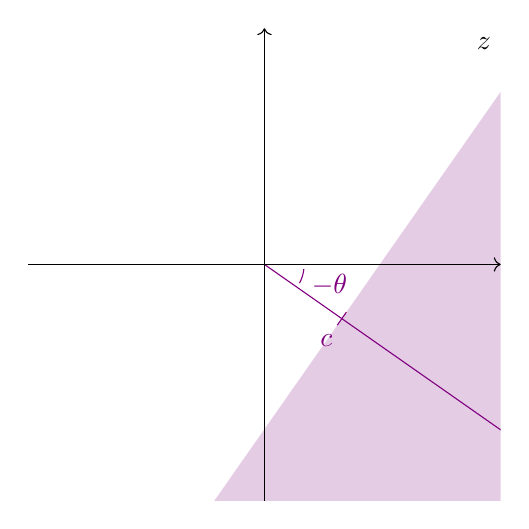
\begin{tikzpicture}
\newcommand{\size}{3}
\pgfmathsetmacro{\outsize}{sqrt(2)*\size}
\newcommand{\ang}{35}
\newcommand{\dis}{1.2}
\begin{scope}
  \clip (-\size, -\size) rectangle (\size, \size);
  \fill[violet!20, rotate=-\ang] (\dis, -\outsize) rectangle (\outsize, \outsize);
  \begin{scope}[violet]
    \draw (0, 0) -- (-\ang:\outsize);
    \draw[rotate=-\ang] (\dis, -0.1) -- (\dis, 0.1);
    \draw[shorten <=0.6mm, shorten >=0.6mm] (0:0.5) arc (0:-\ang:0.5) node[midway, anchor=180-\ang/2] {$-\theta$};
    \node[anchor=90-\ang, inner sep=2mm] at (-\ang:\dis) {$c$};
  \end{scope}
\end{scope}
%%\begin{scope}[violet]
%%  \draw (0, 0) -- (center);
%%  \fill (center) circle (0.05);
%%\end{scope}
\draw[->] (-\size, 0) -- (\size, 0);
\draw[->] (0, -\size) -- (0, \size);
\node[anchor=north east] at (\size, \size) {$z$};
\end{tikzpicture}
\end{center}
When the half-plane extends along the $-\theta$ direction, the sum $\hat{f}$ of the Borel transform of $\aexp^{-\theta} F$ has an absolutely convergent Laplace transform along the $\theta$ direction. In fact, we have $|\hat{f}| \lesssim e^{c |\zeta|}$ uniformly over all $\zeta$ in a constant-radius neighborhood of the ray $e^{i\theta}[0, \infty)$.
\begin{center}
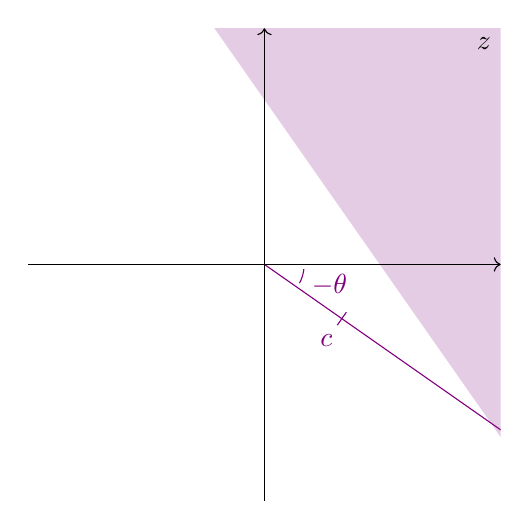
\begin{tikzpicture}
\newcommand{\size}{3}
\pgfmathsetmacro{\outsize}{sqrt(2)*\size}
\newcommand{\ang}{35}
\newcommand{\dis}{1.2}
\begin{scope}
  \clip (-\size, -\size) rectangle (\size, \size);
  \fill[violet!20, rotate=\ang] (\dis, -\outsize) rectangle (\outsize, \outsize);
  \begin{scope}[violet]
    \draw (0, 0) -- (-\ang:\outsize);
    \draw[rotate=-\ang] (\dis, -0.1) -- (\dis, 0.1);
    \draw[shorten <=0.6mm, shorten >=0.6mm] (0:0.5) arc (0:-\ang:0.5) node[midway, anchor=180-\ang/2] {$-\theta$};
    \node[anchor=90-\ang, inner sep=2mm] at (-\ang:\dis) {$c$};
  \end{scope}
\end{scope}
%%\begin{scope}[violet]
%%  \draw (0, 0) -- (center);
%%  \fill (center) circle (0.05);
%%\end{scope}
\draw[->] (-\size, 0) -- (\size, 0);
\draw[->] (0, -\size) -- (0, \size);
\node[anchor=north east] at (\size, \size) {$z$};
\end{tikzpicture}
\end{center}

%%a function $\Phi$ holomorphic in a sectorial neighbourhood $\mathsf{A}_\theta:=\{z\in\C \vert \Re(e^{i\theta}z)\}$ is Borel regular. Indeed let $\series{\Phi}\in\C\llbracket z^{-1}\rrbracket$ be the ``Gevrey-asymptotics'' of $\Phi$ as $\Re(e^{i\theta}z)\to \infty$, then its Borel transform $\hat{\phi}\defeq\borel\series{\Phi}$ is a germ of holomorphic function at the origin and it can be analytically continued in a tubular neighbourhood of the ray $e^{i\theta}[0,\infty)$ with at most exponential growth at infinity. Hence $\Phi$ is Borel-regularizable. In addition, $\series{\phi}$ converges uniformly to a holomorphic function $\phi(\zeta)$ whose Laplace transform coincides with $\Phi(z)$. In particular, we learn that being ``Gevrey-asymptotic'' to a formal series is a sufficient condition for Borel regularity. 
\subsubsection{Borel regularity sometimes explains why Borel summation works}\label{borel-reg:explanatory-power}
The idea of Borel regularity can help us understand why Borel summation is so effective in some situations. Roughly speaking, Borel summation works well for problems with Borel regular solutions that stand out asymptotically \textcolor{magenta}{[this may need refining]}.

The central goal of this paper is to explain, from this perspective, why Borel summation works well for the two kinds of problems exemplified in Section~\ref{intro:summation}.
\begin{enumerate}
\item Solving a linear ODE of single level~$1$ \cite[Section 2.1]{EcalleIII}\textcolor{DarkTurquoise}{\cite[Section~5.2.2.1]{diverg-resurg-iii}}. One example is Equation~\eqref{eqn:bessel-rescaled-1}. The general example is the equation $\mathcal{P} \Phi = 0$ given by a differential operator of the form
\[ \mathcal{P} = P(\partial_z) + \frac{1}{z} Q(\partial_z) + \frac{1}{z^2}\big[ R_0(z^{-1}) + R_1(z^{-1})\,\partial_z + \ldots + R_{d-1}(z^{-1})\,\partial_z^{d-1} \big], \]
where $P$ is a monic degree-$d$ polynomial, $Q$ is a degree-$(d-1)$ polynomial, and $R_0, \ldots, R_{d-1}$ are entire functions of exponential type (i.e. $|R_j(z)|<C_j e^{a_j|z|}$ as $|z|\to+\infty$, for $C_j,a_j>0$ ).

We'll restrict our attention to the case where the roots of $P$ are distinct.

The form of $\mathcal{P}$ derives from Equation~2.2.3 \textcolor{orange}{(p.~105)} of \cite{EcalleIII}, which encompasses both linear and nonlinear ODEs of level $1$. Borel summation still works well for the nonlinear ones, raising the question of whether our analysis generalizes.

\item the second problem is evaluating a certain kind of exponential integral: a one-dimensional {\em thimble integral}

\begin{equation}
I(z)\defeq\int_{\Lambda}\exp\big[-z f\big] \nu
\end{equation}
where $f\colon X\to \mathbb{C}$ is a Morse function, $X$ is $1$-dimensional complex algebraic variety, $\nu\in\Omega^1(X)$ is holomorphic $1$-form in $X$ and $\Lambda$ is a suitable contour such that $I(z)$ is a holomorphic function of $z$.  
\end{enumerate}

These two problems are closely linked. By playing with derivatives of an exponential integral, you can often find a linear ODE that the integral satisfies. Conversely, for many classical ODEs, there are useful bases of exponential integral solutions.

%Notice that our starting point is quite different: we assume $\Phi$ is a holomorphic functions such that it is either a thimble integral or it solves an ODE with irregular singularity at $\infty$. Then we prove $\Phi$ is Borel regular and in both cases, our proves follow the heuristic of the diagram above. We will give precise statements in the following section.

       



%%\item {\em A priori}, we should expect $\hat{\Phi}$ to be different from $\Phi$, because we lose information in passing from $\Phi$ to its asymptotic series.
%%\item Taking the Borel sum of the asymptotic series of $\Phi$ is a regularization process, because it smooths away some perturbations---the ones that are asymptotic to zero along the given ray. We'll call it {\em Borel regularization}.
%%\item Taking the Borel sum of the asymptotic series of $\Phi$ can be seen as a regularization process, because taking asymptotics erases information. We'll call this process {\em Borel regularization}.
%\begin{itemize}
%\item We'll say $\Phi$ is {\em Borel-regularizable} if it's asymptotic to a Borel-summable power series.
%\item We'll say $\Phi$ is {\em Borel regular} if it's Borel-regularizable and Borel regularization leaves it unchanged.
%\item We have the following vector space inclusions:
%\[ \text{Borel regular functions} \subset \text{Borel-regularizable functions} \subset \text{holomorphic functions}. \]
%\item Borel regular functions have been characterized in the literature before; Watson showed a century ago \textcolor{orange}{[Watson]} that a function $\Phi$ is Borel regular whenever there's a constant $c \in (0, \infty)$ with
%\[ |\Phi(z)-\sum_{k=0}^Nc_kz^{-k}| \le c^{N+1} N!|z|^{-N} \]
%over all orders $N$ and all $z$ in a wide enough wedge around infinity. 
%
%Nevanlinna's improvement of Watson's theorem (Sokal, ``An improvement of Watson's theorem on Borel summability'') tells us that for a function $\Phi$ with a well-defined inverse Laplace transform $\phi$, the following conditions are equivalent \textcolor{magenta}{[double check]}:
%\begin{itemize}
%\item $\Phi$ is Borel regular.
%\item $\Phi$ is approximated well, in a certain sense (a weak version of being ``Gevrey-asymptotic''), by its asymptotic series.
%\item $\phi$ grows at most exponentially along the Laplace transform ray.
%\end{itemize}
%\item When its domain is restricted to the space of Gevrey power series, Borel summation is invertible. \textcolor{magenta}{[Need to find a good reference for this, because a small change in the statement would mess up our conclusion. Does \texttt{arXiv:2112.08792}, \S A.2 have the statement we want?]} Thus, Borel regularization acts as a projection operator on the space of Borel-regularizable functions.\textcolor{orange}{[Veronica: Do you mean that if $\Phi\sim\tilde{\Phi}$ and $\tilde{\Phi}$ is Gevrey and Borel summable, then $\Phi=\laplace\circ\borel\tilde{\Phi}$ (i.e. it is Borel regular)? P.Ramis proved that if $\Phi$ is Gevrey asymptotic to $\tilde{\Phi}$, then $\tilde{\Phi}$ is of Gevrey type. In addition, every Gevrey type series $\tilde{\Phi}$ is the Gevrey asymptotics of a holomorphic function. When it is defined, the Borel sum of $\tilde{\Phi}$ is the natural holomorphic function asymptotic to $\tilde{\Phi}$.]}
%\item Borel regularity can help explain why Borel summation is so effective at solving certain kinds of problems, like the ones in Section~\ref{intro:summation}.
%\item The formal solutions of a problem are typically supposed to generalize the actual solutions, in the sense that they include the asymptotic series of the actual solutions.
%\item In this case, every Borel regular solution can be found by taking the Borel sum of a formal solution.
%\item \ldots
%\end{itemize}



\subsection{Goals and Results}

First of all we want to clearly separate the parts of the theory that deal with holomorphic functions and formal series. Indeed, for ODEs, we can build an analytic frame of solutions with an explicit growth behaviour (see Theorem~\ref{thm1}), while for thimble integrals we can write an explicit analytic function whose Laplace transform is the thimble integral itself (see part 3 of Theorem~\ref{thm:maxim}). 

Second of all, we want to explain why it is useful to work in the Borel plane (the spatial domain): on the one hand integral equations are more regular than differential equations. On the other hand, a thimble integral in the frequency domain can be recast as the Laplace transform of a function in the spatial domain. 

\subsubsection{Why does Borel summation work for solutions of single level-$1$ ODEs?}
As described in Section~\ref{borel-reg:explanatory-power}, we consider a linear single level-$1$ ODE $\mathcal{P}\Phi = 0$ given by a differential operator of the form
\begin{equation}\label{eqn:standard ODE}
\mathcal{P} = P(\partial_z) + \frac{1}{z} Q(\partial_z) + \frac{1}{z^2}\big[ R_0(z^{-1}) + R_1(z^{-1})\,\partial_z + \ldots + R_{d-1}(z^{-1})\,\partial_z^{d-1} \big],
\end{equation}
where $P$ is a monic degree-$d$ polynomial, $Q$ is a degree-$(d-1)$ polynomial, and $R_0(z^{-1}), \ldots, R_{d-1}(z^{-1})$ are holomorphic in some disk $|z| > A$ around $z = \infty$.\footnote{Looking at the existence theorem in {\tt airy-resurgence} 2.1.3, we could apply this reasoning on the analytic side for more general equations, but this particular case makes it easier to talk about the formal side as well.]} Furthermore we assume $P$ has simple zeros $P(-\alpha_j)=0$, $j=1,...,d$, $P'(-\alpha_j)\neq 0$ for $j=1,...,d$ and $Q(-\alpha_j)\neq 0$. Our equation has an irregular singularity at $\infty$ \textcolor{magenta}{[Verify this more carefully! It seems like there should be $2(d-1)$ Stokes sectors, as described below]}.

\color{DarkTurquoise}
In \cite[Proposition~2.2.7]{EcalleIII}, where
\begin{align*}
P(\lambda) & = P_0 + P_1 \lambda + \ldots + P_d \lambda^d \\
Q(\lambda) & = Q_0 + Q_1 \lambda + \ldots + Q_{d-1} \lambda^{d-1}
\end{align*}
(with the coefficients renamed to avoid a conflict with the zeros $\alpha_j$), the recurrence that gives the solution simplifies
\begin{align*} b_q & = P_q + Q_q z^{-1} - \frac{\partial}{\partial x^{(q)}} b(z, x, x^{(1)}, \ldots x^{(d)}) \\
& = P_q + Q_q z^{-1} - R_q(z^{-1}).
\end{align*}

Following the argument of Delabaere Lemma~6.2, we can prove that $\series{F}_j(z)$ is $1$-Gevrey by taking the formal Borel transform of the ODE it satisfies and showing it is regular singular at $\zeta=0$. 

Roughly speaking, factoring out $e^{-\alpha_j z}$ removes the constant term of $P$, and factoring out $z^{-\tau_j}$ changes $Q$ to give factorial growth instead of gamma function growth (?).

\begin{align*}
\mathcal{P} & = \sum_j^d f_j \frac{\partial}{\partial z}^j \\
& = \sum_j^d f_j \left(-\frac{1}{w^2} \frac{\partial}{\partial w}\right)^j\\
&=  \sum_j^d \tilde{f}_j \frac{\partial}{\partial w}^j
\end{align*}
where $w=1/z$.  if $\tilde{f}_j $ has a pole of order at most $d-j$ at 0 then it's regular singular, otherwise it's irregular. The relevant term should be
\color{Tan}
\[ \left(\frac{P_d}{w^{2d}} + \frac{R_d(w)}{w^{2d-2}}\right) \left(\frac{\partial}{\partial w}\right)^d , \]
\color{DarkTurquoise}
\[ \frac{P_d}{w^{2d}}  \left(\frac{\partial}{\partial w}\right)^d , \]
corresponding to the quadratic differential $dw^2/w^{2d}$, whose trajectories form $2(d-1)$ half-planes around $\infty$ (see Bridgeland \& Smith's ``Quadratic differential as stability conditions,'' Figure~10).

From the Bessel equation, for example, we get
\begin{align*}
(-w^{-2}\partial_w)^2&=-w^{-2}\partial_w(-w^{-2}\partial_w)\\
&=-w^{-2}(2w^{-3}\partial_w-w^{-2}\partial_w^2)\\
&=-2w^{-5}\partial_w+w^{-4}\partial_w^2,
\end{align*}
giving two half-planes around $\infty$, as expected.
\color{black}

Under these assumptions, the space of formal solutions of $\mathcal{P}\Phi = 0$ has a basis $\series{\Psi}_1,...,\series{\Psi}_d$ of the form~\cite{int-irreg}\cite[Proposition~2.2.7, p.~111]{EcalleIII}
\begin{equation}\label{formal solution}
\series{\Psi}_j(z)=e^{-\alpha_j z}z^{-\tau_j}\series{F}_j(z)\in e^{-\alpha_j z } z^{-\tau_j}\,\C \llbracket z^{-1} \rrbracket,
\end{equation}
where $\tau_j$ is the non-zero complex number $Q(-\alpha_j)/P'(-\alpha_j)$. Since the roots $-\alpha_1, \ldots, -\alpha_n$ are distinct, this form determines the basis up to scaling, giving the space of formal solutions a distinguished frame.

Classically it was proved that the formal solutions of \eqref{formal solution} are Borel-Laplace summable and their Borel-Laplace sums satisfy the original differential equation (see for example \cite{ramis1991series,malgrange92,malgrange1995sommation,diverg-resurg--ii}\textcolor{magenta}{[Braaksma,check]}). Therefore, the distinguished frame of formal solutions $\series{\Psi}_1,...,\series{\Psi}_d$ becomes a distinguished frame of analytic solutions $\hat{\Psi}_1,...,\hat{\Psi}_d$.       

However, can we find a distinguished basis for solutions in a purely analytic way? This should be possible because of our regularity assumptions about the coefficients of $\mathcal{P}$. In fact, the Main Asymptotic Existence Theorem (M.A.E.T.) guarantees the existence of an analytic frame of solutions asymptotic to a formal frame (see \cite[Theorem 3.1]{diverg-resurg-iii}), but it is not a constructive method (see \cite[Chapter 14]{balser}). Conversely, we can explicitly build a distinguished basis of analytic solutions: 

\begin{theorem}[see Theorem \ref{thm1-dim}]\label{thm1}
In the previous set-up, for every $\alpha_j$ we set $\zeta_j=\zeta-\alpha_j$. Then, there exists a unique solution of $\hat{P}_j\psi_j=0$ with 

\begin{equation}
\hat{P}_j:=P(-\alpha_j-\zeta_j)+\partial_{\zeta,\alpha_j}^{-1}\circ Q(-\alpha_j-\zeta_j)+\partial_{\zeta,\alpha_j}^{-2}\circ\sum_{r=0}^{d-1}R_r(\partial_{\zeta,\alpha_j}^{-1})\circ (-\alpha_j-\zeta_j)^r
\end{equation}

such that $\psi_j$ blows-up as $\zeta^{\tau_j-1}$ at $\alpha_j$:
${\psi}_j(\zeta_j)=\zeta_j^{-\tau_j-1}+f_j$ and $f_j\in\mathcal{HL}^{\infty,-\tau_j}(\Omega)$ for a small compact domain $\Omega\subset\C$. 
\end{theorem}


At this point, we may ask what is the relationship between the two frame of analytic solutions, namely the Borel sum $\hat{\Psi}_j$ of the formal solutions $\series{\Psi}_j$ and the Laplace transform of $\psi_j$. Our main result says they are actually the same, hence proving Borel summation works. 
 
\begin{theorem}\label{thm2}
For every $j=1,...,d$ the solution $\psi_j(\zeta_j)$ of Theorem \ref{thm1} admits a well defined Laplace transform $\Psi_j:=\laplace_{\zeta_j}^{\theta_j}$ for some direction $\theta_j$.
Furthermore, $\tilde{\Psi}_j$ is Borel summable and its Borel sum is proportional to $\Psi_j$. 
\end{theorem}

In fact, $\Psi_j$ is a Borel regular solution of \eqref{eqn:standard ODE}.  

In the following diagram, we sketch the main step of the proof of Theorem~\ref{thm2}: on the right-hand side of the diagram, we have the formal solution $\series{\Psi }_j$ and its Borel transform $\series{\psi}_j$. Then, the theory of $1$-summability allows us to draw the ``square'' with corners $\hat{\psi}_j$ and its Laplace transform $\hat{\Psi}_j$.  

\begin{center}
\begin{tikzcd}
& & ODE\arrow[dd,"\borel"]\arrow[dd,"\laplace^{-1}",swap] & & \\
\Psi\arrow[rru,dotted, no head, tail] &\textcolor{red}{\hat{\Psi}}\arrow[ur,red, no head, tail] & & & \tilde{\Psi}\arrow[llu,"formal",swap, no head, tail]\arrow[dd,"\borel"]\\
& & IE & & \\
\psi\arrow[rru, no head, tail]\arrow[uu,"\laplace"]& \textcolor{red}{\hat{\psi}}\arrow[ur, no head, tail]\arrow[rrr,"sum",mapsfrom,red]\arrow[uu,"\laplace"]& & & \tilde{\psi}\arrow[llu, no head, tail]
\end{tikzcd}
\end{center} 

Conversely, on the left-hand side, we have the unique (up to scaling) analytic function $\psi_j$ of Theorem~\ref{thm1} which solves the integral equation (IE) obtained as the inverse Laplace transform of the (ODE).   

The key step is then comparing $\psi_j$ and $\hat{\psi}_j$. First, using properties of the Borel transform, it is easy to show that $\series{\psi}_j$ is a formal solution of the integral equation (IE), hence its sum $\hat{\psi}_j$ must be a solution too. In addition, from the explicit formula for $\tilde{\Psi}_j$, we can show that $\hat{\psi}_j$ grows as $\zeta^{-\tau_j+1}$ near $\zeta=\alpha_j$
therefore, by our uniqueness result~\ref{thm1}, we conclude that $\psi_j$ and $\hat{\psi}_j$ must coincide up to scaling by a constant. 

As a consequence, by properties of the Laplace transform, $\Psi_j\defeq\laplace_{\zeta_j}^{\theta}\psi_j$ is an analytic solution of the (ODE) and it is asymptotic to $\series{\Psi}_j$. Furthermore, $\Psi_j$ is proportional to $\hat{\Psi}_j$.   

\begin{remark}
There are many ways to build a frame of solutions for these kinds of ODEs: formally in the $z$-plane Poincar\'e gave an explicit solution \cite{int-irreg}. Formally in the $\zeta$-plane \'Ecalle figured out how to find a frame of formal solutions of the Borel transformed ODE \textcolor{magenta}{[add reference]\cite{EcalleIII,loday-Remy2011}}. It can indeed be seen as a consequence of ``resurgence'' of the ODE. Our results show how to build a frame of solutions, analytically in the Borel plane. Furthermore, it shows we are picking the same frame: from the properties of the Laplace transform we get an analytic frame asymptotic to Poincar\'e frame $\series{\Psi}_j$. From the uniqueness result of Theorem~\ref{thm1}, we get a frame of analytic solutions equivalent to \'Ecalle's ones. 
\end{remark} 

\color{Tan}
\begin{remark}
Although, in our proof, we use $1$-summability to ensure that the Borel sum of the formal solution $\series{\Psi}_j$ exists and it solves the ODE, the approach of Borel regularity is different as it is based on the analytic solution in the frequency domain ($z$-plane). \textcolor{magenta}{[Is it possible to prove Borel regularity without proving Borel summability? For instance, can we argue that $\psi_j$ being the unique solution of (IE) with a certain behavior is enough to say that it is the sum of $\series{\psi}_j$? Check carefully the argument of multi-summability]} 
\end{remark}

\color{magenta}
[Veronica]

Although, in our proof, we adapt an argument by M. Loday-Richaud and P. Remy (see \S 2 in\cite{loday-Remy2011}) to guarantee Borel--Laplace summability, the approach of Borel regularity is different as it is based on the analytic solution in the frequency domain ($z$-plane). In addition, our proof stresses the importance of the position domain, where in fact the crucial step of the proof is done. 

%\color{gray}
%\begin{itemize}
%\item Can we see there exists a distinguished basis in a purely analytic way? YES. %%[Thm 1]% The reason is the existence theorem gives for every $\alpha_j$ a unique solution in the $\zeta$-plane which blows-up in a certain way at $\alpha_j$: ${\phi}_j(\zeta_j)=\zeta_j^{-\tau_j}+\tilde{f}_j$, $\zeta_j=\zeta-\alpha_j$.
%\item why Borel summations of $\tilde{\Psi_1},...,\tilde{\Psi_d}$ finds this solutions? because they are an analytic frame of Borel regular functions. 
%\end{itemize}
%\begin{itemize}
%\item {[Thm 1]}: for every $\alpha_j$ there exists a unique solution in the $\zeta$-plane which blows-up in a certain way at $\alpha_j$: ${\phi}_j(\zeta_j)=\zeta_j^{-\tau_j}+\tilde{f}_j$, $\zeta_j=\zeta-\alpha_j$. (proof based on existence theorem \ref{frac_int_exist})
%\item {[Thm 2]}: The Borel sum of the formal solutions $\tilde{\Psi}_j$ are the same as the Laplace transform of the solutions of Thm 1. 
%\item Cor of Thm 2: the Laplace transform of solutions of Thm 1 are Borel regular.   
%\item Say there's a unique solution (up to scaling) that shrinks as you go right; everything else blows up exponentially. Then this is the only solution that can be expressed as a Laplace transform. [Follows from Aaron's argument in Airy resurgence, even if Aaron works with more general ODEs]

%\item Draw diagram showing formal vs. holomorphic solutions in time vs. frequency domains.

%\begin{center}
%\begin{tikzcd}
%& & ODE\arrow[dd,"\borel"]\arrow[dd,"\laplace^{-1}",swap] & & \\
%\Phi\arrow[rru,dotted, no head, tail] &\textcolor{red}{\hat{\Phi}}\arrow[ur,red, no head, tail] & & & \tilde{\Phi}\arrow[llu,"formal",swap, no head, tail]\arrow[dd,"\borel"]\\
%& & IE & & \\
%\phi\arrow[rru, no head, tail]\arrow[uu,"\laplace"]& \textcolor{red}{\hat{\phi}}\arrow[ur, no head, tail]\arrow[rrr,"sum",mapsfrom,red]\arrow[uu,"\laplace"]& & & \tilde{\phi}\arrow[llu, no head, tail]
%\end{tikzcd}
%\end{center}

%where the arrow in red are a consequence of multisummability. In addition, we can distinguish on the right hand side of the diagram the formal solutions and on the left hand side the holomorphic ones. On the upper part of the diagram the functions in the $z$-plane while on the lower part the functions in the Borel plane $\zeta$-plane.
%\item  
%there are many ways to see this problem have a distinguished base of solutions, Poincar\'e see it formally in the $z$-plane, \textcolor{red}{Ecalle figured it out how to see it formally in the Borel plane}, our results shows how to see it analytically in  the Borel plane.
%\item  M.A.E.T. says you can start in formal $z$-plane but it is not really constructive (see Balser chap 14); going from formal $\zeta$ to analytic is constructive and it's essentially Borel-Laplace summation. Our method uses just Laplace transform. 
%\item How do we know we are picking the same frame? from properties of Laplace transform we get solution asymptotics to Poincar\'e frame. From uniqueness result we get a frame equivalent to Ecalle's frame. 
%\item multi-summability is a regularity result starting form the formal solution in the $z$-plane. Borel regularity is instead based on the analytic solution in the $z$-plane. The argument we gave about getting the same frame is what proves Borel regularity of $\Psi_j$.   
%\end{itemize}

\color{black}

\subsubsection{Why does Borel resummation work for thimbles integrals?}

\color{DarkBlue}
\begin{itemize}
%\item This is the setup. Let $X$ be an algebraic variety of dimension $N$, $f\colon X\to \mathbb{C}$ be a holomorphic Morse function with only simple critical points and $\nu\in\Gamma(X,\Omega^N)$.
%\begin{itemize}
%\item recall theory of homology and cohomology to define the thimbles integrals. Pham has briefly discussed it, but apparently was introduced by Malgrange, Milnor and ?.  
%\end{itemize} 
\item background: Pham studied the asymptotic behaviour of thimble integrals and we may interpret his result as a prof of Borel regularity in the algebraic setting, namely assuming $f$ a polynomial with distinct critical points (not necessary non--degenerate), $X=\C^N$, $\nu=g(x)dx_1\wedge...\wedge dx_N$ with $g(x)$ a polynomial. His proof uses microlocal analysis and classical results due to Varchenko. In the same algebraic setting, Malgrange states the Borel regularity result Theorem 6 \cite{Malgrange22} 
\item \textcolor{red}{We give an explicit proof of Borel regularity beyond the polynomial case. Indeed I think we can simply assume $f$ holomorphic and proper.}
\item I think we should separate what can we do in general for N-dimensional integral and what is special for the $1$-dimensional one. 
%\item {[Thm 4]} 1-dim thimbles integrals are Borel regular, namely let 
%\begin{equation}
%I_{\alpha}(z)\defeq\int_{\Lambda_\alpha}e^{-zf}\nu
%\end{equation}

%then the following diagram is commutative
%\begin{equation}
%\begin{tikzcd}
%I_{\alpha}(z) \arrow[r,"\aexp^\theta"] & \tilde{I}_{\alpha}(z)\arrow[dd,"\borel"]\\
%& \\
%\hat{\iota}_\alpha(\zeta)\arrow[uu, "\laplace^\theta_\alpha "] & \tilde{\iota}_{\alpha}(\zeta) \arrow[l, "\text{sum}"]
%\end{tikzcd}
%\end{equation}
\begin{itemize}
%\item on the one hand take asymptotic expansion of integral via saddle point approximation and then study the Borel Laplace sum of the divergent series [from left upper corners clockwise]
\item on the other hand \textcolor{red}{see that the thimble integral is a generalized Laplace transform (which in certain cases can be rewritten as a usual Laplace transform).}
\item A priori, the Laplace transform of $\hat{\iota}_\alpha(\zeta)$ and $I_{\alpha}(z)$ have the same asymptotic behaviour in a given sector (indeed taking the asymptotic of $I_\alpha(z)$ we \textit{loose} information); however Borel regularity guarantees that $I_{\alpha}(z)=\laplace^{\theta}\hat{\iota}_{\alpha}$ in a given sector.
\item A corollary of [Thm 4] is the thimble projection formula.
\item \textcolor{red}{As a consequence of Thm 2.4 Pham}, if $f$ and $\nu$ are algebraic, we get that $\hat{\varphi}_\alpha(\zeta)$ to have simple singularities 
\begin{equation}
mmm
\end{equation} 
\end{itemize}
\item \text{[Cor]:} combining our result and the result of Maxim [IHES lectures] (generalizing Pham) we can deduce that Stokes constants for the Borel--Laplace sum of $\tilde{I}_j(z)$ are always integers as they are intersection numbers (use same argument of Maxim). See also the argument of KS21 sec 6.2 in the framework of analytic WCFs. 
\begin{itemize}
\item Prove integrality of Stokes constants using the fractional integral formula vs differential equation (see example in Appendix C) 
\end{itemize}
\end{itemize}
\color{black}

Let $X$ be an $N$-dimensional complex algebraic variety and $f\colon X\to\mathbb{A}^1$ be a proper algebraic map with non--degenerate critical points $\alpha_1,...,\alpha_N$ \footnote{Everything we will discuss, applies also when $X$ is a $N$-dimensional complex (K\"ahler) manifold and $f\colon X\to\C$ is a holomorphic function with non-degenerates critical points, which is, for example, the setting in \cite{Witten}.}: for a fixed $z\in\C$, we are interested in integrals of the form 

\[
I(z):=\int_{\mathcal{C}}e^{-zf}\nu
\]

regarded as holomorphic functions in the position domain for a suitable choice of a contour $\mathcal{C}$ and an $N$-form $\nu$. In fact, we introduce homology and cohomology groups $H_{*}^{B,z}$ and $H_{dR,z}^*$ so that the function $I(z)$ will represent the Poincar\'e pairing. 

We begin with the definition of $H_{*}^{B,z}$: it is the relative homology group with respect to $zf$, and its definition requires some preliminaries. We follow \cite{pham} and $\S 1$ in \cite{Arnold}. Let us fix $z\in\C$ and $\theta=\arg z$; for every $c>0$ we define 
\begin{align*}
    S_c^+(\theta) &:=\lbrace \zeta\in\C \vert \Re (\zeta e^{i\theta})\geq c \rbrace\\
    S_c^-(\theta)&:=\lbrace \zeta\in\C \vert \Re (\zeta e^{i\theta})\leq c \rbrace
\end{align*}
and $H_{*}^{B,z}:=H_{*}(X,f^{-1}(S_c^+(\theta)))$ for $c$ large enough\footnote{In fact $H_{*}^{B,z}$ is defined after taking the projective limit $c\to\infty$ of the chain complex with support $\{A\subset X \text{ closed s.t. } \forall c>0 f^{-1}(S_c^-(\theta))\cup A \text{ is compact }  \}$.}. Moreover, $H_n(X,f^{-1}(S_c^+(\theta)))$ can be identified with the homology of a generic fiber $H_{n-1}(f^{-1}(p_0))$ with $p_0\neq \{\alpha_j\}$. This leads to further identifications:

\begin{equation}
    H_{*}^{B,z}\cong \bigoplus_{\alpha_i} H_{*}(B_j, B_j^+(\theta))
\end{equation}
where $B_j:=f^{-1}(B_r(\alpha_j))$ is the preimage of a small ball or radius $r$, containing only the critical value $\alpha_i$ and $B_j^+(\theta):=f^{-1}\left(B_r(\alpha_j)\cap \{ \Re (\zeta e^{i\theta})\geq r/2\}\right)$. Notice that we are not assuming $f$ to be Morse, hence $B_j$ may have different connected components. Then 

\begin{equation}
    H_{n}(B_j, B_j^+(\theta))\cong H_{n-1}(f^{-1}(p_j))\cong \begin{cases} \Z^{\mu_j} & \text{if } n=N\\
     0 & \text{otherwise}
    \end{cases}
\end{equation}
where $|p_j-\alpha_j|=r$, $\Re(p_j e^{i\theta})=r$ and $\mu_j$ is the Milnor number of the critical point $\alpha_j$. 


\begin{center}
    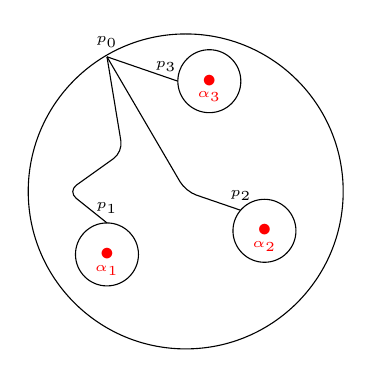
\begin{tikzpicture}
        \draw (2,2) circle (2);
        \node[font=\tiny,red] at (1,1) {$\alpha_1$};
        \draw (1,1.2) circle (0.4);
        \node[font=\tiny,red] at (3,1.3) {$\alpha_2$};
        \draw (3,1.5) circle (0.4);
        \node[font=\tiny,red] at (2.3,3.2) {$\alpha_3$};
        \draw (2.3,3.4) circle (0.4);
        \node[above,red] at (1,1) {$\bullet$};
        \node[above,red] at (3,1.3) {$\bullet$};
        \node[above,red] at (2.3,3.2) {$\bullet$};
        \draw[rounded corners] (2.7,1.76)--(2,2)--(1,3.71);
        \draw[rounded corners] (1,1.6)--(0.5,2)--(1.2,2.5)--(1,3.71);
        \draw[rounded corners] (1.9,3.4)--(1,3.71);
        \node[font=\tiny, above] at (1,3.71) {$p_0$};
        \node[font=\tiny, above] at (2.7,1.76) {$p_2$};
        \node[font=\tiny, above] at (1,1.6) {$p_1$};
        \node[font=\tiny, above] at (1.75,3.4) {$p_3$};
    \end{tikzpicture}
\end{center}

From the classical theory of singularities \cite{Arnold} we know that $H_{N-1}(f^{-1}(p_0))$ has a distinguished basis of \textit{vanishing cycles} from the generic fiber over $p_0$ to the preimage of each critical value. 
Moreover, the vanishing cycles can be identified with the so-called \textit{Lefschetz thimbles}: since we assumed critical points to be non--degenerate, in a neighborhood of $\alpha_j$ there are local coordinates $x_1,...,x_N$ such that 
\[f=\alpha_j+\sum_{k=1}^N x_k^2\]

and for $p=c e^{i\theta}\in\C$, the thimble $\Lambda_j(p)$ is defined by 
\begin{align*}
    \Im(x_1)=...=\Im(x_N)=0 \text{ and } \Re(e^{-i\theta/2}x_1)^2+....+\Re(e^{-i\theta/2}x_N)^2\leq c
\end{align*}
Equivalently, Lefschetz thimbles are gradient flow trajectories departing from the critical points of $f$ (see \cite{Witten} page 10).

Hence we deduce that $H_{z, N}^B$ admits a distinguished basis of Lefschetz thimbles labeled by critical points.


Then we recall the definition of $H_{dR,z}^\cdot$: it is the hypercohomolgy of the twisted de Rham complex 

\begin{equation*}
    H_{dR,z}^*:=\mathbb{H}^*( \Omega^\bullet(X), zd+df)
\end{equation*}
where $(\Omega^\bullet(X), d)$ is the de Rham complex of differential forms on $X$. 

Therefore, the integral $I(z)$ can e regarded as the image of the following map: 

\begin{align*}
    \int \colon  H_{z,N}^{B} \times & H_{dR,z}^N \to \C \\
       [\mathcal{C}] ,\,\, & [\nu] \to \int_{\mathcal{C}}e^{-zf}\nu
\end{align*}

\textcolor{orange}{[the Betti--de Rham isomorphism is necessery?]}

Since every cycle $\mathcal{C}$ can be written as a linear combination of Lefschetz thimbles, we restrict our attention to  \textit{thimbles} integrals $I_\alpha$, namely the integrals over Lefschetz thimbles labeled by the critical points $x_j\in\text{Crit}(f)$.

As we let $z$ vary, we will observe the so-called \textit{Stokes phenomena}, namely the integral $I_j(z)$ jumps across the rays $\ell_{jl}=\arg(\alpha_j-\alpha_l)\R_{\geq 0}$ for $l=1,...,k$ (and $l\neq j$). The jumps can be described geometrically using the theory of Picard--Lefschetz. Indeed, the jumps of $I_j(z)$ are encoded in the jumps of the Lefschetz thimbles $[\Lambda_j]\in H_{z,N}^B$ as $\arg z$ varies.   


Now using the steepest descendent method we can compute the asymptotic expansion of thimble integrals which in general gives a formal series $\tilde{I}_\alpha$ (see Malgrange, Pham, and for more general thimble integrals see \cite[Section 1.2.2]{mistegard_phdthesis} and \cite{andersen2020resurgence}, the Stirling series for Gamma function in \cite{Maxim_slide_ERC,Maxim_talk_2023}).

Our goal is to study whether $\tilde{I}_j$ is Borel summable and whether its Borel--Laplace sum agrees with the integral $I_j$. 

These questions have been classically addressed by Pham (\S 3.3 \cite{pham}), Malgrange (Theorem 6 in \cite{Malgrange22}), Delabere and Pham \cite{Delabaere-Pham99}, Berry and Howls \cite{berry1991hyperasymptotics}, Dunne and Unsal \cite{dunne-unsal}, and others. \textcolor{orange}{[add references]} 

Our approach wants to focus on the role of the position domain and it emphasizes how the geometry of the Laplace transform is the natural framework to describe Borel regularity for thimbles integrals (see Fenyes's lecture \cite{Fenyes-ihes-lecture}).  

We will restrict to $1$-dimensional thimble integrals, and in this special case we will define our setting in the language of translation surfaces, to make clear the connection with our geometric picture of the Laplace transform. 
\color{DarkBlue}
Let $X$ be a translation surface---a Riemann surface carrying a holomorphic 1-form $\nu$. Suppose $X$ is of {\em meromorphic type}, meaning that we got it by puncturing a compact Riemann surface $\overline{X}$ at finitely many points, and $\nu$ has a pole at each puncture. A {\em translation coordinate} on $X$ is a local coordinate whose derivative is $\nu$. Take another meromorphic-type translation surface $B$ and a holomorphic map $f \maps \overline{X} \to \overline{B}$ with non--degenerate critical points \textcolor{magenta}{that sends punctures to punctures [actually, don't require this; the Orr--Sommerfeld integrals, for example, don't satisfy it]}. \textcolor{red}{Suppose every singularity of $B$ is a critical value of $f$.[Veronica: Is it a good assumption?]} \textcolor{DarkGreen}{\textbf{[Typical usage of ``Borel plane'' seems ambiguous, so maybe we can use ``Borel plane'' for $B$ and ``Borel cover'' for the Riemann surface of the Borel-transformed series. How to handle the Orr–Sommerfeld functions (\cite{dlmf}~\S 9.13)? We know $f = 4u^3 - 3u$ is the pullback of a translation coordinate, but we also need a puncture at $f(0)$\ldots]}} 
\color{black}
For each critical point $x_j$, let $\Gamma_j$ be the ray going rightward from the critical value $\alpha_j:=f(x_j)$, and let $\zeta_{\alpha_j}$ be the translation coordinate around $\Gamma_j$ which vanishes at $\alpha_j$. These are well-defined as long as $\Gamma_j$ misses the critical values of $f$. The preimage $f^{-1}(\Gamma_j)$ is a bunch of disjoint curves (see Figure \ref{fig:thimble_vs_rays}), as long as $\Gamma_j$ misses the other critical values of $f$. The Lefschetz thimble  $\Lambda_j$ can be regarded as the component of $f^{-1}(\Gamma_j)$ that goes through $x_j$, \textcolor{orange}{oriented so that shifting it to its left would make its projection run clockwise around $\Gamma_j$}. 

\begin{figure}[h]
    \centering
    %\includegraphics{}
    \caption{The preimage of a ray departing from the critical value and going to infinity.}
    \label{fig:thimble_vs_rays}
\end{figure}

%The {\em thimble integral}
%\[ I_p = \int_{\Lambda_p} e^{-z f^*\zeta_p} \nu \]
%is a holomorphic function on the right half-plane parametrized by $z$, and it turns out to be Borel regular.

Then, our main result for thimble integrals is proving that $1$- dimensional thimble integrals are indeed Borel regular:

\begin{theorem}[see Theorem \ref{thm:maxim}]
    Let $\tilde{I}_{j}(z)\defeq e^{-z \alpha_j}(2\pi)^{1/2} z^{-1/2} \sum_{n\geq 0}a_{j,n}z^{-n}$ be the asymptotic expansion of $I_j$ as $\Re z e^{i\theta}\to \infty$ for a generic direction $\theta$. Then:
\begin{enumerate}
\item The series $\tilde{\Phi}_j:=z^{1/2} \tilde{I}_j$ is $1$-Gevrey, thus $\tilde{\phi}_j(\zeta)\defeq\borel_\zeta(\tilde{\Phi}_j)$ converges near $\zeta=\alpha_j$
\item If you continue the sum of $\tilde{\phi}_j$ along the ray going rightward from $\alpha_j$, and take its Laplace transform along that ray, you'll recover $z^{1/2} I_j$.
\item For any $\zeta$ on the ray going rightward from $\alpha_j$, we have
\begin{multline}
\hat{\phi}_{j}(\zeta)=\fracderiv{\textcolor{red}{3/2}}{\zeta}{\alpha_j} \left( \int_{\Lambda_j(\zeta)}\nu \right)=\textcolor{red}{\left(\tfrac{\partial}{\partial \zeta}\right)^2}\,\frac{1}{\Gamma\big(\tfrac{1}{2}\big)} \int_{\alpha_j}^\zeta (\zeta-\zeta')^{-1/2} \textcolor{red}{\left( \int_{\Lambda_j(\zeta')} \nu \right)}\,d\zeta',
\end{multline}
where $\Lambda_j(\zeta)$ is the part of $\Lambda_j$ that goes through $f^{-1}([\alpha_j, \zeta])$. Notice that $\Lambda_j(\zeta)$ starts and ends in $f^{-1}(\zeta)$. \textbf{[Be careful about the orientation of $\Lambda_j$.]}
\end{enumerate}
\end{theorem}

The idea of the proof is sketched below in the following diagram:
\[
\begin{tikzcd}
{I}_{j} \arrow[rrr,"\aexp"]\arrow[dd, swap,"\laplace^{-1} "] &  & & \tilde{I}_{j}\arrow[dd,"\borel"]\\
& & &\\
\iota_j \arrow[r,equal] & \hat{\iota}_j & &\tilde{\iota}_{j} \arrow[ll, "\text{sum}"]
\end{tikzcd}
\]

on the one hand, the thimble integral $I_j$ can be regarded as a Laplace type integral, i.e. as the Laplace transform of a function $\iota_j$. In addition, $\iota_j$ can be written explicitly in an integral formula \eqref{formula1}. 
On the other hand, reading the diagram from the right-hand side, we compute the asymptotic expansion of $I_j$ using the saddle point approximation, which turns out to be a formal $1$-Gevrey series. Thus, its Borel transform $\series{\iota}_j$ is a germ of holomorphic functions at $\alpha_j$ which can be summed to a holomorphic function $\hat{\iota}_j$. At this point, we realize that $\iota_j$ and $\hat{\iota}_j$ are indeed the same. In a nutshell, thimble integrals are Borel regular because they can be turned into Laplace transforms.      


In higher-dimensional complex manifolds, integrals over Lefschetz thimbles \textcolor{red}{[I'm not so sure]} are still Borel regular~\textbf{[``Exponential integrals, Lefschetz thimbles and linear resurgence''][``Exponential Integral'' lectures?]}. This fact plays an important technical role in quantum mechanics, where infinite-dimensional exponential integrals are supposed to give the expectation values of observable quantities. Physicists often use Borel summation, resurgence and related techniques to assign values to these integrals \textbf{[Costin \& Kruskal, ``On optimal truncation...''],\cite{delabaere-howls,dingle1973asymptotic}[Delabere \& Howls, Howls, Dingle]}.


%Choose a path $\gamma \maps \R \to X$ whose projection $f \circ \gamma$ starts out going leftward out of a puncture, ends up going rightward into a puncture, and never touches a critical value of $f$. Choose a translation coordinate $\zeta$ on $B$ and continue it along $f \circ \gamma$, noting that it may become multi-valued if $f \circ \gamma$ intersects itself. This data defines the {\em exponential integral}
%\[ I = \int_\gamma e^{-z f^*\zeta} \nu, \]
%a holomorphic function on the right half-plane parametrized by $z$. It turns out \textbf{[we hope]} that we can get $I$ by summing $e^{-\alpha_p z} I_p$ over various critical points---as long as none of the $\Gamma_p$ run into each other. \textbf{[We get jumps at phases where the $\Gamma_p$ do hit each other.]} The constants $\alpha_p$ are values of $\zeta$, continued to the critical points along certain paths.



\subsubsection{Other results}

As part of the treatment, we have made use of some new perspectives on the Laplace transform (see Section~\ref{sec:Laplace-Borel-general}). Indeed, the Laplace transform is often used to solve ODEs on the frequency domain by relating them to ODEs on the spatial domain. We find, however, that it is much easier and more natural to relate ODEs on the frequency domain to integral equations on the spatial domain. In particular, working with integral equations in the spatial domain will be our main strategy to prove Borel regularity for ODEs (see Theorem~\ref{thm1}). Our approach is different from the one of Malgrange in \cite{malgrange--fourier} where he uses differential equations in the spatial domain. 

Furthermore, we introduce a geometric picture where the spatial domain $B$ is a translation surface. If $b \in B$ is non-singular, the frequency domain for $\laplace_b^\theta$ is $T^* B_b$. If $b$ is a conical singularity, the frequency domain is more interesting, as we'll see in our main example (see Figure \ref{fig:different_fibres}). 


\begin{figure}[h]
    \centering
    %\includegraphics[]{}
    \caption{The fiber over an ordinary point of the translation surface $B$ is a copy of the complex plane. However, the fiber over a singular point of $B$ has an interesting structure. Here we represent the example of Airy functions.}
    \label{fig:different_fibres}
\end{figure}

We will illustrate our main results with detailed treatments of several examples: we will mostly focus on degree two ODEs that admit a frame of solutions expressed as thimble integrals (the Airy--Lucas functions, modified Bessel function, Airy function, the anharmonic oscillator...). Then, on the one hand, we explicitly solve the integral equation associated with the ODE, building a frame of analytic solutions as the Laplace transform of the solutions of the integral equation. On the other hand, our \textit{thimble projection reasoning} shows how to rewrite explicitly thimble integrals as a Laplace transform and it makes Borel regularity evident directly from explicit computations.

Among the examples we study, some of them have been discussed many times, using different approaches and conventions. We try to give an idea of how all these different treatments fit together. For instance, for the Airy function we will make a comparison with \S 2.2 in \cite{lectures-Marino}, \S 6.14 in \cite{diverg-resurg-i}, and \S 2.2 \cite{kawai-takei}). The anharmonic oscillator was also discussed in (Bender--Wu, Appendix B in \cite{aniceto2019primer}). Other examples haven't been discussed much, as for Airy--Lucas functions. 

 
Recently, resurgence theory (first developed by \'Ecalle in the '80) has attracted interest in mathematics and physics as a powerful alternative to Borel summability. The resurgence of linear ODEs have been intensively studied (see Costin slides for ReNewQuantum, \cite{EcalleIII,loday1994stokes}) and many results are also known for non-linear ODEs (see \cite{schiappa-PI}, \cite{costin-PI} \textcolor{magenta}{[check also paper by Ecalle and Sauzin]}). For algebraic thimble integrals of the type we studied in this paper, resurgence of their asymptotic expansion can be understood geometrically (see \cite{Maxim_slide_ERC}, \S 6.2 in \cite{kontsevich2022analyticity}), however for more general exponential integrals (see examples in \cite{Maxim_slide_ERC}) resurgence remains a conjecture. Despite their simplicity, our examples of linear ODEs and of 1-dimensional integrals show some features of resurgence and they are toy-model to get a feeling of \'Ecalle formalism. 

%\color{gray}
%\begin{itemize}
%\item The central goal of this paper is to lay out two kinds of problems where we can prove that the Borel sum of a formal power series solution is always an actual solution.
%\begin{itemize}
%\item The first problem is evaluating a certain kind of exponential integral: a one-dimensional {\em thimble integral}.
%\item The second problem is solving a certain kind of ODE.
%\item These two problems are closely linked. By playing with derivatives of an exponential integral, you can often find a linear ODE that the integral satisfies. Conversely, for many classical ODEs, there are useful bases of exponential integral solutions.
%\item \textcolor{magenta}{(Does this touch the Picard-Lefshetz perspective? Betti / de Rham relationship: ODE is a connection, and exponential integrals give flat sections?)}
%\end{itemize}
%
%\item Clearly separate the parts of the theory that deal with holomorphic functions and formal power series.
%\begin{itemize}
%\item we can do that also for thimble integrals (this is part 4 of Thm 5.1 in {\tt draft2.pdf})
%\end{itemize}
%\item (Super-motivation: why do the zeroes of $\lambda$ play a special role?) As part of the treatment, we've made use of some new perspectives on the Laplace transform.
%\begin{itemize}
%\item \textbf{Geometric picture.} The spatial domain $B$ is a translation surface. If $b \in B$ is non-singular, the frequency domain for $\laplace_b^\theta$ is $T^* B_b$. If $b$ is a conical singularity, the frequency domain is more interesting, as we'll see in our main example.
%\item \textbf{A new dictionary for ODEs.} The Laplace transform is often used to solve ODEs on the frequency domain by relating them to ODEs on the spatial domain. We find, however, that it's much easier and more natural to relate ODEs on the frequency domain to integral equations on the spatial domain. 
%\begin{itemize}
%\item This clarifies why we take the Borel sums at zeroes of $\lambda$ when we're trying to solve an ODE.
%\end{itemize}
%\end{itemize}
%\item Our picture helps explain why it's useful to work on the Borel plane (the position domain).
%\begin{itemize}
%\item Integral equations are more regular than differential equations.
%\item A thimble integral in the frequency domain can be recast as the Laplace transform of a function in the position domain.
%\end{itemize}
%\item Illustrate with detailed treatments of several examples.
%\begin{itemize}
%\item Contour argument (thimble integrals)
%\item solving integral equation (ODE)
%\item How thimble integrals and ODE are related in our examples?
%\end{itemize}
%\begin{itemize}
%\item Some have been discussed many times, using different approaches and conventions. We'll try to give an idea of how all these different treatments fit together. $\bullet$ The Airy function (Marino, Sauzin). $\bullet$ The anharmonic oscillator (Bender--Wu, Schiappa).
%\item Others haven't been discussed much.
%\end{itemize}
%\item Recently, resurgence theory (first developed by \'Ecalle in the '80) has attracted interests in math and physics as a powerful alternative to Borel summability. Resurgence of lienar ODEs have been studied (see Costin slides for ReNewQuantum). Many results are also known for non linear ODEs (see Schiappa PI, Costin PI). For algebraic exponential integrals of the type we studied in this paper, resurgence of their asymptotic expansion can be understood geometrically (see Maxim's slides ReNewQuantum), however for more general exponential integrals (see examples in Maxim's talk) resurgence remains a conjecture. Despite their simplicity, our examples of linear ODEs and of exponential integrals show some features of resurgence and they are toy model to get a feeling on \'Ecalle formalism.       
%\item \textcolor{magenta}{The examples give a place to compare more complicated formalisms like the Picard-Lefshetz (Morse theory) or Ecalle formalisms? [How do we work this into the introduction?]}
%\begin{itemize}
%\item thimble integrals are geometric in the sense of being pairing between homology and cohomology 
%\item computation of Stokes constants via Picard--Lefschetz theory
%\end{itemize}
%\end{itemize}
\subsection{Results}

\color{orange}
\begin{itemize}
\item what does it mean to be Borel regular?
\item when does it happen?
\begin{itemize}
\item State new Borel regularity results
\begin{itemize}
\item Linear, homogeneous ODE with a regular singularity at 0 and irregular singularity at infinity [big idea in {\tt airy-resurgence}]
\begin{itemize}
\item Contextualize with previous work of Braaksma (``Multisummability and Stokes multipliers of linear meromorphic differential equations'')
\item Also contextualize with Balser, Braaksma, Sibuya, and Ramis (``Multisummability of formal power series solutions of linear ordinary differential equations'')
\item Also contextualize with Loday-Richaud
\end{itemize}
\item \emph{Borel regularity} for \textbf{thimbles integrals} can be stated a the commutativity of the following diagram:
\begin{equation}
\begin{tikzcd}
I_{\alpha}(z)\defeq\int_{\mathcal{C}_\alpha}e^{-zf}\nu \arrow[r,"\sim"]\arrow[dd, swap, "\laplace^\theta "] & \tilde{I}_{\alpha}(z)\arrow[dd,"\borel"]\\
& \\
\hat{\iota}_\alpha(\zeta)\arrow[r,equal,swap, "\text{sum}"] & \tilde{\iota}_{\alpha}(\zeta) 
\end{tikzcd}
\end{equation}
\item A priori, the Laplace transform of $\hat{\iota}_\alpha(\zeta)$ and $I_{\alpha}(z)$ have the same asymptotic behavior in a given sector (indeed taking the asymptotic of $I_\alpha(z)$ we \textit{loose} information); however Borel regularity guarantees that $I_{\alpha}(z)=\laplace^{\theta}\hat{\iota}_{\alpha}$ in a given sector.
\item thimble projection formula
\item Conjecturally, we expect $\hat{\varphi}_\alpha(\zeta)$ to have simple singularities. 
\item in the examples, $\hat{\varphi}_\alpha(\zeta)$ turn out be an hypergeometric function of type ${}_pF_{p-1}$ where $p$ is the number of critical values. 
\item We expect that hypergeometric functions play a special role in resurgence theory as they may always appear when there are only finitely many singularities.
\item \textcolor{magenta}{maybe we can say more about algebraic hypergeometric functions}
\end{itemize}
%\item Recall Watson condition (old): Let $R_N$ be the difference between a function and the partial sum
%\[ \frac{\varphi_0}{z} + \frac{\varphi_1}{z^2} + \frac{\varphi_2}{z^3} + \ldots + \frac{\varphi_{N-2}}{z^{N-1}} \]
%of its asymptotic series. Watson showed a century ago that the function is Borel regular whenever there's a constant $c \in (0, \infty)$ with
%\[ |R_N| \le \frac{c^{N+1} N!}{|z|^N} \]
%over all orders $N$ and all $z$ in a wide enough wedge around infinity.
\end{itemize}
\end{itemize}

%\subsection{Why does Borel resummation work?}
%
%\color{gray}
%
%Borel resummation is a way of turning a formal power series
%\[ \series{\varphi} = z^\sigma \left( \frac{\varphi_0}{z} + \frac{\varphi_1}{z^2} + \frac{\varphi_2}{z^3} + \frac{\varphi_3}{z^4} + \ldots \right), \]
%with $\sigma \in [0, 1)$, into a function which is asymptotic to $\series{\varphi}$ as $z \to \infty$. Different functions can be asymptotic to the same power series, and Borel resummation picks one of them, performing an implicit regularization~\textbf{[arXiv:1705.03071, or maybe arXiv:1412.6614]}. When a function matches the Borel sum of its asymptotic series, we'll say it's {\em Borel regular}. Several familiar kinds of regularity imply Borel regularity, and shed light on why it occurs.
%%%Knowing that a function is Borel regular gives us extra information about it---enough to reconstruct it from its asymptotic series. What's the nature of this extra information?
%%%Since different functions can be asymptotic to the same power series, Borel resummation must involve an {\em implicit regularization}, restricting its range to a class of functions which are uniquely determined by their formal power series.
%\begin{itemize}
%\item \textbf{Having a good asymptotic approximation}
%
%Let $R_N$ be the difference between a function and the partial sum
%\[ \frac{\varphi_0}{z} + \frac{\varphi_1}{z^2} + \frac{\varphi_2}{z^3} + \ldots + \frac{\varphi_{N-2}}{z^{N-1}} \]
%of its asymptotic series. Watson showed a century ago that the function is Borel regular whenever there's a constant $c \in (0, \infty)$ with
%\[ |R_N| \le \frac{c^{N+1} N!}{|z|^N} \]
%over all orders $N$ and all $z$ in a wide enough wedge around infinity (Sokal, ``An improvement of Watson's theorem on Borel summability''; Hardy, {\em Divergent Series}, Theorem~136; Watson, ``A theory of asymptotic series,'' \S 8?).
%\color{black}
%
%\item \textbf{Satisfying a singular differential equation}
%
%\begin{itemize}
%\item This is the setup. We restrict to ODEs with irregular singularity at $\infty$ and of Poincaré rank $1$: 
%\begin{equation}\label{eqn:standard ODE}
%\Big[ P(\partial_z)+\frac{1}{z}Q_1(\partial_z)+\sum_{j=2}^d z^{-j}R_j(\partial_z)\Big]\Psi=0
%\end{equation}
%where $P(\lambda)$ is a (monic) degree $d$ polynomial, $Q(\lambda)$ is a degree $d-1$ polynomial and $R_j$ is a degree $d-j$ polynomial. \textcolor{magenta}{[Looking at the existence theorem in {\tt airy-resurgence} 2.1.3, we could apply this reasoning on the analytic side for more general equations, but this particular case makes it easier to talk about the formal side as well.]} Furthermore we assume $P$ has simple zeros $P(\alpha_j)=0$, $j=1,...,d$ and $Q(\alpha_j)\neq 0$.
%\item \color{DarkTurquoise}
%I think we can go more general? If I'm not mistaken, \'{E}calle's equation form \cite[Equation~2.2.3, p.~105]{EcalleIII} covers operators like
%\[ P(\partial_z) + \frac{1}{z} Q_1(\partial_z) + \frac{1}{z^2}\big[ R_0(z^{-1}) + R_1(z^{-1})\,\partial_z + \ldots + R_d(z^{-1})\,\partial_z^d \b], \]
%where $P$ and $Q$ are as above, and $R_0, \ldots, R_d$ are holomorphic functions on $\C$.
%\color{black}
%\item (backgrounds) Under these assumptions, 
%\begin{itemize}
%\item \eqref{eqn:standard ODE} admits a basis of formal solutions: let $\tau_j:=Q(-\alpha_j)/P'(-\alpha_j)\in\mathbb{Q}^*$, then the formal solutions $\tilde{\Psi}_1,...,\tilde{\Psi}_d$ are of the form \cite{int-irreg} \cite[Proposition~2.2.7, p.~111]{EcalleIII}
%\begin{equation}
%\label{formal solution}
%\tilde{\Psi}_j(z)=e^{-\alpha_j z}z^{-\tau_j}\tilde{F}_j(z)\in e^{-\alpha_j z } z^{-\tau_j}\,\C \llbracket z^{-\tau_j} \rrbracket
%\end{equation}
%Notice that this basis is distinguished only up to scaling, so we have a distinguished frame in the space of formal solutions. 
%\item \eqref{formal solution} is Borel-Laplace summable and its Borel-Laplace sum $\Psi_j$ satisfies the original equation \eqref{eqn:standard ODE}
%\item as a consequence, the distinguished frame of formal solutions become a distinguished frame of analytic solutions $\Psi_1,...,\Psi_d$.  
%\end{itemize}
%\item Can we see there exists a distinguished basis in a purely analytic way? YES. [Thm 1]% The reason is the existence theorem gives for every $\alpha_j$ a unique solution in the $\zeta$-plane which blows-up in a certain way at $\alpha_j$: ${\phi}_j(\zeta_j)=\zeta_j^{-\tau_j}+\tilde{f}_j$, $\zeta_j=\zeta-\alpha_j$.
%\item why Borel summations of $\tilde{\Psi_1},...,\tilde{\Psi_d}$ finds this solutions? because they are an analytic frame of Borel regular functions. 
%\begin{itemize}
%\item {[Thm 1]}: for every $\alpha_j$ there exists a unique solution in the $\zeta$-plane which blows-up in a certain way at $\alpha_j$: ${\phi}_j(\zeta_j)=\zeta_j^{-\tau_j}+\tilde{f}_j$, $\zeta_j=\zeta-\alpha_j$. (proof based on existence theorem \ref{frac_int_exist})
%\item {[Thm 2]}: The Borel sum of the formal solutions $\tilde{\Psi}_j$ are the same as the Laplace transform of the solutions of Thm 1. 
%\item Cor of Thm 2: the Laplace transform of solutions of Thm 1 are Borel regular.   
%\end{itemize}
%\item Say there's a unique solution (up to scaling) that shrinks as you go right; everything else blows up exponentially. Then this is the only solution that can be expressed as a Laplace transform. [Follows from Aaron's argument in Airy resurgence, even if Aaron works with more general ODEs]
%
%\item Draw diagram showing formal vs. holomorphic solutions in time vs. frequency domains.
%
%\begin{center}
%\begin{tikzcd}
%& & ODE\arrow[dd,"\borel"]\arrow[dd,"\laplace^{-1}",swap] & & \\
%\Phi\arrow[rru,dotted, no head, tail] &\textcolor{red}{\hat{\Phi}}\arrow[ur,red, no head, tail] & & & \tilde{\Phi}\arrow[llu,"formal",swap, no head, tail]\arrow[dd,"\borel"]\\
%& & IE & & \\
%\phi\arrow[rru, no head, tail]\arrow[uu,"\laplace"]& \textcolor{red}{\hat{\phi}}\arrow[ur, no head, tail]\arrow[rrr,"sum",mapsfrom,red]\arrow[uu,"\laplace"]& & & \tilde{\phi}\arrow[llu, no head, tail]
%\end{tikzcd}
%\end{center}
%
%where the arrow in red are a consequence of multisummability. In addition, we can distinguish on the right hand side of the diagram the formal solutions and on the left hand side the holomorphic ones. On the upper part of the diagram the functions in the $z$-plane while on the lower part the functions in the Borel plane $\zeta$-plane.
%\item  
%there are many ways to see this problem have a distinguished base of solutions, Poincar\'e see it formally in the $z$-plane, \textcolor{red}{Ecalle figured it out how to see it formally in the Borel plane}, our results shows how to see it analytically in  the Borel plane.
%\item  M.A.E.T. says you can start in formal $z$-plane but it is not really constructive (see Balser chap 14); going from formal $\zeta$ to analytic is constructive and it's essentially Borel-Laplace summation. Our method uses just Laplace transform. 
%\item How do we know we are picking the same frame? from properties of Laplace transform we get solution asymptotics to Poincar\'e frame. From uniqueness result we get a frame equivalent to Ecalle's frame. 
%\item multi-summability is a regularity result starting form the formal solution in the $z$-plane. Borel regularity is instead based on the analytic solution in the $z$-plane. The argument we gave about getting the same frame is what proves Borel regularity of $\Psi_j$.   
%\end{itemize}
%
%\color{DarkBlue}
%
%\item \textbf{Being a thimble integral}
%
%\begin{itemize}
%\item This is the setup. Let $X$ be an algebraic variety of dimension $N$, $f\colon X\to \mathbb{C}$ be a holomorphic Morse function with only simple critical points and $\nu\in\Gamma(X,\Omega^N)$.
%\begin{itemize}
%\item recall theory of homology and cohomology to define the thimbles integrals. Pham has briefly discussed it, but apparently was introduced by Malgrange, Milnor and ?.  
%\end{itemize} 
%\item background: Pham prove Borel regularity for exponential integral in N-dimension and without assuming Morse critical points (but only isolated). His proof is geometric [it may be useful to add it in Appendix]. 
%\item \textcolor{red}{We give an analytic proof analogous of Pham.}
%\item I think we should separate what can we do in general for N-dimensional integral and what is special for the $1$-dimensional one. 
%\item {[Thm 4]} 1-dim thimbles integrals are Borel regular, namely let 
%\begin{equation}
%I_{\alpha}(z)\defeq\int_{\Lambda_\alpha}e^{-zf}\nu
%\end{equation}
%
%then the following diagram is commutative
%\begin{equation}
%\begin{tikzcd}
%I_{\alpha}(z) \arrow[r,"\ae^\theta"] & \tilde{I}_{\alpha}(z)\arrow[dd,"\borel"]\\
%& \\
%\hat{\iota}_\alpha(\zeta)\arrow[uu, "\laplace^\theta_\alpha "] & \tilde{\iota}_{\alpha}(\zeta) \arrow[l, "\text{sum}"]
%\end{tikzcd}
%\end{equation}
%\begin{itemize}
%\item on the one hand take asymptotic expansion of integral via saddle point approximation and then study the Borel Laplace sum of the divergent series [from left upper corners clockwise]
%\item on the other hand \textcolor{red}{see that the thimble integral is a generalized Laplace transform (which in certain cases can be rewritten as a usual Laplace transform).}
%\item A priori, the Laplace transform of $\hat{\iota}_\alpha(\zeta)$ and $I_{\alpha}(z)$ have the same asymptotic behaviour in a given sector (indeed taking the asymptotic of $I_\alpha(z)$ we \textit{loose} information); however Borel regularity guarantees that $I_{\alpha}(z)=\laplace^{\theta}\hat{\iota}_{\alpha}$ in a given sector.
%\item A corollary of [Thm 4] is the fractional derivative formula.
%\item Conjecturally, we expect $\hat{\varphi}_\alpha(\zeta)$ to have simple singularities. 
%\end{itemize}
%\item From the result of Pham we can deduce Stokes constants are always integers as they are intersection numbers (use same argument of Maxim). See also the argument of KS21 sec 6.2 in the framework of analytic WCFs. Prove integrality of Stokes constants using the fractional integral formula vs differential equation (see example in Appendix C) 
%\end{itemize}


\color{black}


\subsection{thimble projection formula}
\begin{itemize}
\item formula \eqref{formula1} Theorem~\ref{thm:maxim} says that for a certain class of exponential integrals
\[ I(z) = \int_\Gamma e^{-zf}\;\nu, \]
the inverse Laplace transform is the $\tfrac{3}{2}$ derivative of $\nu/df$ at $\zeta=f$.
\item the asymptotic expansion of $I(z)$ is a resurgent function.
\item Is it always a \emph{simple} resurgent function?
\begin{itemize}
\item \textbf{Maxim belies it is in general, and indeed in our examples, we get simple resurgent functions. But how to prove it in general?}
\end{itemize} 
\end{itemize}

%\subsection{Stokes phenomenon}
%\begin{itemize}
%\item For Bessel functions, we can see explicitly how solutions jump when the Laplace transform angle crosses a critical value.
%\item The jump comes from the branch cut difference identity for hypergeometric functions.
%\item Possible interpretation of the Stokes factors as intersections numbers in Morse--Novikov theory \textbf{[ask Maxim]}
%\end{itemize}
\section{The Laplace and Borel transforms}\label{sec:Laplace-Borel-general}
\subsection{The geometry of the Laplace transform}

Classically, the Laplace transform turns functions on the position domain into functions on the frequency domain. In the study of Borel summation and resurgence, it's useful to see the position domain as a {\em translation surface} $B$, and the frequency domain as one of its cotangent spaces. Roughly speaking, the Laplace transform lifts holomorphic functions on $B$ to holomorphic functions on $T^* B$.
\subsubsection{Translation surfaces, briefly}

A translation surface is a Riemann surface $B$ carrying a holomorphic $1$-form $\lambda$~\cite{zorich2006flat}. A translation chart is a local coordinate $\zeta$ with $d\zeta = \lambda$. The standard metric on $\C$ pulls back along translation charts to a flat metric on $B$, with a conical singularity of angle $2\pi n$ wherever $\lambda$ has a zero of order $n-1 > 0$. We'll require $B$ to be finite-type and $\lambda$ to have a pole at each puncture. This kind of translation surface has a ``cylindrical end'' \textbf{(figure)} at each puncture where $\lambda$ has order $-1$, and a ``$|2n|$-planar end'' \textbf{(figure)} at each puncture where $\lambda$ has order $n-1 < -1$~\cite{gupta2013meromorphic} \S 2.5] (or cite Aaron's article, which will hopefully present the same background in the translation surface context).
\subsubsection{Direction}\label{transl:dir}
The translation structure gives $B$ a notion of direction as well as distance. Away from the zeros of $\lambda$, which we'll call {\em branch points}, we can talk about moving upward, rightward, or at any angle, just as we would on $\C$. At a branch point of cone angle $2\pi n$, we can also talk about moving upward, rightward, or at any angle in $\R/2\pi\Z$, but here there are $n$ directions that fit each description. To make this more concrete, note that around any point $b \in B$, there's a unique holomorphic function $\zeta_b$ that vanishes at $b$ and has $d\zeta_b = \lambda$. \textcolor{VioletRed}{[If we define ``translation parameter'' earlier, we can say:] there's a unique translation parameter $\zeta_b$ that vanishes at $b$.} This function is a translation chart when $b$ is an ordinary point, and an $n$-fold branched covering when $b$ is a branch point of cone angle $2\pi n$. In either case, $\zeta_b \in e^{i\theta} [0, \infty)$ is a ray or a set of rays leaving $b$ at angle $\theta \in \R/2\pi\Z$.

Near each branch point $b$, let's fix a coordinate $\omega_b$ with $\zeta_b = \tfrac{1}{n} \omega_b^n$, where $2\pi n$ is the cone angle at $b$. This lets us label each direction at $b$ with an ``extended angle'' in $\R/2\pi n\Z$. Of course, there are $n$ different choices for $\omega_b$.

\subsubsection{Frequency}\label{transl-freq}

The translation structure also gives us an isomorphism $z \maps T^*B_b \to \C$ when $b \in B$ is an ordinary point, and an isomorphism $z \maps T^*B_b^{\otimes n} \to \C$ when $b$ is a branch point of cone angle $2\pi n$. At an ordinary point, we can define $z$ simply as the map
\begin{align*}
z \maps T^*B_b & \to \C \\
\lambda\big|_b & \mapsto 1.
\end{align*}
To get a definition that generalizes to branch points, though, it's worth taking a fancier point of view. Recall that $T^*B_b = \van_b / \van_b^2$, where $\van_b$ is the ideal of holomorphic functions that vanish at $b$. Observing that $(f + \van_b)^n$ lies within $f^n + \van_b^{n+1}$ for any $f \in \van_b$, we can identify $T^*B_b^{\otimes n}$ with $\van_b^n / \van_b^{n+1}$ for $n \ge 1$. When $b$ is an ordinary point, the function $\zeta_b$ defined in Section~\ref{transl:dir} represents a nonzero element of $\van_b / \van_b^2$: the cotangent vector $\lambda\big|_b$. In general, $\zeta_b$ represents a nonzero element of $\van_b^n / \van_b^{n+1}$, where $2\pi n$ is the cone angle at $b$. We define $z$ as the isomorphism
\begin{align*}
z \maps \van_b^n / \van_b^{n+1} & \to \C \\
\zeta_b + \van^{n+1} & \mapsto 1.
\end{align*}

When $b$ is a branch point, the coordinate $\omega_b$ we chose in Section~\ref{transl:dir} gives us an isomorphism
\begin{align*}
w_b \maps T^*B_b & \to \C \\
\omega_b + \van^2 & \mapsto 1
\end{align*}
that makes the diagram
\begin{center}
\begin{tikzcd}
T^*B_b^{\otimes n} \arrow[r,"z"] & \C \\
T^*B_b \arrow[u,"\blankbox^n"] \arrow[r,"w"'] & \C \arrow[u,"\blankbox^n"']
\end{tikzcd}
\end{center}
commute.
\subsubsection{Boundary}
\textbf{Discuss the visual boundary, citing Lemma~3.1 of Dankwart's thesis \textit{On the large-scale geometry of flat surfaces} for the description of geodesics.}

\subsubsection{The Laplace transform over an ordinary point}%%\label{laplace:ordinary}
Pick a local holomorphic function $\zeta$ on $B$ with $d\zeta = \lambda$, and an extended angle $\theta \in \R$. \textcolor{VioletRed}{[If we define ``translation parameter'' earlier, we can say:] Pick a translation parameter $\zeta$.} The {\em Laplace transform} $\laplace_\zeta^\theta$ turns a local holomorphic function $f$ on $B$ into a local holomorphic function on $T^*B$. When $b \in B$ is an ordinary point, $\laplace_\zeta^\theta f$ is defined on $T^*B_b$ by the formula
\begin{equation}\label{laplace:int}
\laplace_\zeta^\theta f\big|_b = \int_{\Gamma_b^\theta} e^{-z\zeta} f\,d\zeta,
\end{equation}
where $z$ is the frequency function and $\Gamma_b^\theta$ is the ray that leaves $b$ at angle $\theta$. We will use the shorthand $\laplace_{\zeta, b}^\theta f := \laplace_\zeta^\theta f \big|_{\zeta = b}$ throughout this document.

To make sense of this formula, we ask for the following conditions.
\begin{itemize}
\item The base point $b$ is in the domain of $\zeta$. Once we have this, we can continue $\zeta$ along the whole ray $\Gamma_b^\theta$.
\item The ray $\Gamma_b^\theta$ avoids the branch points after leaving $b$.
\item The integral converges. We guarantee this by asking for a pair of simpler conditions.
\begin{itemize}
\item With respect to the flat metric, $f$ grows subexponentially along $\Gamma_b^\theta$~\textbf{[define]}, and is locally integrable throughout.
\item The value of $z$ is in the half-plane $H_{-\theta}$ centered around the ray $e^{-i\theta} [0, \infty)$.
\end{itemize}
\end{itemize}
\subsubsection{The Laplace transform over a branch point}
When $b$ is a branch point, we can still use formula~\ref{laplace:int} to define $\laplace_\zeta^\theta f$ on $T^*B_b$, as long as we take care of a few subtleties. Thanks to the labeling choices we made at the end of Section~\ref{transl:dir}, the extended angle $\theta \in \R$ still picks out a ray $\Gamma_b^\theta$. The function $z$ is defined on $T^*B_b^{\otimes n}$, where $2\pi n$ is cone angle at $b$, so we pull it back to $T^*B_b$ along the $n$th-power map. This amounts to substituting $w_b^n$ for $z$ in formula~\ref{laplace:int}. The half-plane $z \in H_{-\theta}$ in $T^*B_b^{\otimes n}$ pulls back to $n$ sectors of angle $\pi/n$ in $T^*B_b$. We only define $\laplace_\zeta^\theta f$ on one of them: the one centered around the ray $w_b \in e^{-i\theta/n}[0, \infty)$.
%\color{gray}
%\subsection{The geometry of the Borel transform}
%\begin{itemize}
  %\item The Borel transform $\borel\textcolor{orange}{_\zeta}$ turns formal power series in $z^{-1}$---which represent functions defined all non-singular cotangent spaces---into formal power series in $\zeta$. It's a formal inverse of the $\laplace_{\zeta, 0}$.
  %\item Formalizing the change of variable identity that relates $\laplace_{\zeta, \alpha}$ to $\laplace_{\zeta_\alpha, 0}$, we can extend the Borel transform to trans-series, defining $\borel\textcolor{orange}{_\zeta} \maps e^{-\alpha z} \C\llbracket z^{-1} \rrbracket \to \C\llbracket \zeta \rrbracket$ as the formal inverse of $\laplace_{\zeta, \alpha}$.
  %\begin{itemize}
   % \item In other words, when $\borel_\zeta$ acts on formal power series, it formally inverts $\laplace_\zeta$ on the cotangent fiber over $0$. \textcolor{magenta}{When it acts on other trans-monomials, it formally inverts $\laplace_\zeta$ on other cotangent fibers. [Not quite\ldots figure out how to make this precise.] }
  %\end{itemize}
  %\item consequently, $\borel_{\zeta_\alpha}$ acts on trans-monomials $e^{z\alpha}\C\llbracket z^{-1}\rrbracket$ and it formally inverts $\laplace_{\zeta_\alpha}$ on the cotangent fibre over $0$. 
%\end{itemize}
%\color{black}
\subsection{The Laplace transform: analytic version}
\subsubsection{Regularity and decay properties}\label{reg-decay}


Let's say a function $f$ is in $O_{\zeta, \alpha \leftarrow}(g)$ or $O_{\zeta, \alpha \rightarrow}(g)$, respectively, if $|f| \lesssim g$ on some neighborhood of the starting point or infinite end of $\Gamma_{\zeta, \alpha}$. A function is {\em subexponential} along $\Gamma_{\zeta, \alpha}$ if it's in $O_{\zeta, \alpha \rightarrow}(e^{c\zeta})$ for all $c > 0$ \textcolor{magenta}{[shall we write in formula?]}. Let $\mathcal{E}_{\zeta, \alpha}$ be the space of functions that are subexponential on $\Gamma_{\zeta, \alpha}$, integrable at the starting point, and locally integrable throughout. If $f$ is in $\mathcal{E}_{\zeta, \alpha}$, then $\laplace_{\zeta, \alpha} f$ is well-defined and holomorphic for $\Re(z) > 0$ on the part of $T^*B$ that lies over $\Gamma_{\zeta, \alpha}$~\cite[\S 5.6]{diverg-resurg-i}.

The asymptotics of $f$ at the starting point of $\Gamma_{\zeta, \alpha}$ control the asymptotics of $\laplace_{\zeta, \alpha} f$ at the infinite end of $\Gamma_{z, 0}$. Once we see how this works for $\alpha = 0$, Section~\ref{translation} will do the rest. Let $F = \laplace_{\zeta, 0} f$. Equation~1.8 of \cite{laplace-tfm} shows\footnote{The argument cited still works in our generality. For holomorphic $f$, one can also use Equation 1.5 of \cite{sternin1995borel}.} that
\[ f \in O_{\zeta, 0 \leftarrow}(1) \quad\Longrightarrow\quad F \in O_{z, 0 \rightarrow}\left(\frac{1}{z}\right). \]
More generally, for $\tau > -1$ \textcolor{magenta}{[prove or cite]},
\[ f \in O_{\zeta, 0 \leftarrow}(\zeta^\tau) \quad\Longrightarrow\quad F \in O_{z, 0 \rightarrow}\left(\frac{1}{z^{1 + \tau}}\right). \]
Exact power law asymptotics relate similarly \textcolor{magenta}{[prove or cite]}:
\[ f \sim \zeta^\tau \text{ at the start of } \Gamma_{\zeta, 0} \quad\Longrightarrow\quad F \sim \frac{\Gamma(1+\tau)}{z^{1+\tau}} \text{ at the end of } \Gamma_{z, 0}. \]
\textcolor{magenta}{[The big-$O$ asymptotics dictionary is interesting, but we might not need it. Consider dropping.]}


\subsubsection{Change of translation chart}\label{translation}
Define a new coordinate $\zeta_\alpha$ on $B$ so that $\zeta = \alpha + \zeta_\alpha$. From the calculation
\begin{align*}
\laplace_{\zeta, a} \varphi & = \int_{\Gamma_{\zeta, \alpha}} e^{-z \zeta}\,\varphi\;d\zeta \\
& = \int_{\Gamma_{\zeta_\alpha, 0}} e^{-z(\alpha + \zeta_\alpha)}\,\varphi\;d\zeta_\alpha \\
& = e^{-\alpha z} \int_{\Gamma_{\zeta_\alpha, 0}} e^{-z\zeta_\alpha}\,\varphi\;d\zeta_\alpha \\
& = e^{-\alpha z} \laplace_{\zeta_\alpha, 0} \varphi,
\end{align*}
we learn that
\begin{equation}
    \label{change-chart}
    \laplace_{\zeta_\alpha, 0} \varphi = e^{\alpha z} \laplace_{\zeta, \alpha} \varphi.
\end{equation}

\subsubsection{Rescaling of translation structure}

Let us rescale the translation structure of $B$, expanding displacements by a factor of $\mu \in (0, \infty)$. The coordinate $\xi = \mu\zeta$ is a chart for the new translation structure. The corresponding frequency coordinate $x \maps T^*B \to B$ is given by $d\xi \mapsto 1$, so $x = \mu^{-1} z$. From the calculation
\begin{align*}
\laplace_{\xi, 0} \varphi & = \int_{\Gamma_{\xi, 0}} e^{-x\xi}\,\varphi\;d\xi \\
& = \int_{\Gamma_{\zeta, 0}} e^{-z \zeta}\,\varphi\;\mu\,d\zeta \\
& = \mu\,\laplace_{\zeta, 0} \varphi
\end{align*}
we learn that
\[ \laplace_{\xi, 0} \varphi = \mu\,\laplace_{\zeta, 0} \varphi. \]
Note that $\laplace_{\xi, 0}$ is defined in the new translation structure on $B$, while $\laplace_{\zeta, 0}$ is defined in the old translation structure. We can still compare them because they both turn complex-valued functions on $B$ into holomorphic functions on $T^*B$.

\subsubsection{Action on integral operators}\label{L-int-op}
%%For $\nu \in (-\infty, 1)$, the fractional integral $\partial^{\nu-1}_{x \text{ from } 0}$ is defined by
%%\[ \partial^{\nu-1}_{x,0} f(x) \defeq \frac{1}{\Gamma(1-\nu)} \int_0^x (x-x')^{-\nu} f(x')\,dx'. \]
For $\nu \in (-\infty, 1)$, the fractional integral $\partial^{\nu-1}_{\zeta, \alpha}$ is defined by
\[ [\partial^{\nu-1}_{\zeta, \alpha} f](p) \defeq \frac{1}{\Gamma(1-\nu)} \int_{\zeta = \alpha}^p \big(\zeta(p)-\zeta\big)^{-\nu} f\,d\zeta, \]
where $p$ is any point on the position domain $B$. 

It obeys the expected semigroup law \cite[Section  1.3]{mladenov2014advanced}
\begin{align*}
\fracderiv{\lambda}{\zeta}{\alpha}\,\fracderiv{\mu}{\zeta}{\alpha} & = \fracderiv{\lambda+\mu}{\zeta}{\alpha} & \lambda, \mu \in (-\infty, 0),
\end{align*}
and agrees with ordinary repeated integration when $\nu$ is an integer (see equation~35 in \cite{mladenov2014advanced}).

For $\alpha \in (0, 1)$ and integers $n \ge 0$, fractional derivatives $\fracderiv{n+\alpha}{\zeta}{0}$ are defined by composing $\fracderiv{\alpha-1}{\zeta}{0}$ with powers of $\tfrac{\partial}{\partial \zeta}$. However, $\fracderiv{\alpha-1}{\zeta}{0}$ and $\tfrac{\partial}{\partial \zeta}$ don't commute~\cite[equation 54]{mladenov2014advanced}. Various ordering conventions give various definitions of $\fracderiv{n+\alpha}{\zeta}{0} f$, which differ by operators that act on the germ of $f$ at zero (see \cite[\S 1.3]{mladenov2014advanced} \textbf{---original source Podlubny}). We'll use the {\em Riemann-Liouville} convention.
\begin{definition}
For $\alpha \in (0, 1)$ and integers $n \ge 0$, the {\em Riemann-Liouville fractional derivative} $\fracderiv{n+\alpha}{\zeta}{0}$ is defined by
\[ \fracderiv{n+\alpha}{\zeta}{0} \defeq \left(\tfrac{\partial}{\partial \zeta}\right)^{n+1} \fracderiv{\alpha-1}{\zeta}{0}. \]
\end{definition}
The symbol $\fracderiv{\mu}{\zeta}{0}$ is now defined for any $\mu \in \R \smallsetminus \{0, 1, 2, 3, \ldots\}$. It denotes a fractional integral when $\mu$ is negative, and a fractional derivative when $\mu$ is a positive non-integer.

The Riemann-Liouville fractional derivative is a left inverse of the fractional integral, in the sense that $\fracderiv{\lambda}{\zeta}{ 0}\,\fracderiv{-\lambda}{\zeta}{0}=\text{Id}$ for all $\lambda \in (0, \infty)$. This extends the semigroup law:
\begin{align*}
\fracderiv{\lambda}{\zeta}{0}\,\fracderiv{\mu}{\zeta}{0} & = \fracderiv{\lambda+\mu}{\zeta}{0} & \lambda \in \R \smallsetminus \{0, 1, 2, 3, \ldots\},\quad\mu \in (-\infty, 0).
\end{align*}

%Each convention for the fractional derivative brings its own annoyances to interactions with the Borel transform.\footnote{See Remark~\ref{rmk:caputo} for examples.} The Riemann-Liouville derivative will be the least annoying for our purposes. 

%\color{Tan}
%You can use a 2d integration argument, akin to the one in \cite[Theorem~2.39]{laplace-tfm}, to show that $\fracderiv{-\lambda}{\zeta}{a} \varphi \in \mathcal{E}_\zeta$ and
%\[ \laplace_{\zeta, a}\,\fracderiv{-\lambda}{\zeta}{a} \varphi = z^{-\lambda} \laplace_{\zeta, a} \varphi \]
%for all $\lambda \in (0, \infty)$. This generalizes the Laplace transform's action on derivatives: when $\varphi \in \mathcal{E}_\zeta$, you can use differentiation under the integral to show that~\cite[Theorem~1.34]{laplace-tfm}
%\begin{equation}%%\label{id:L-mult}
%\laplace_\zeta (\zeta^n \varphi) = \big({-\tfrac{\partial}{\partial z}}\big)^n \laplace_\zeta \varphi.
%\end{equation}
%for all integers $n \ge 0$.


Using a 2d integration argument, akin to the one in \cite[Theorem~2.39]{laplace-tfm}, one can show that $\partial^{-\lambda}_{\zeta} \varphi \in \mathcal{E}_\zeta$ and
\[ \laplace_{\zeta,0}\,\partial^{-\lambda}_{\zeta} \varphi = z^{-\lambda} \laplace_{\zeta, 0} \varphi \]
for all $\lambda \in (0, \infty)$. This generalizes the Laplace transform's action on derivatives: when $\varphi \in \mathcal{E}_\zeta$, you can use differentiation under the integral to show that~\cite[Theorem~1.34]{laplace-tfm}
\begin{equation}%%\label{id:L-mult}
\laplace_\zeta (\zeta^n \varphi) = \big({-\tfrac{\partial}{\partial z}}\big)^n \laplace_\zeta \varphi.
\end{equation}
for all integers $n \ge 0$.
Furthermore, if $\varphi\in\mathcal{E}_{\zeta,\alpha}$, then $\partial_{\zeta,\alpha}^{-\lambda}\varphi\in\mathcal{E}_{\zeta,\alpha}$ and 
\[ \laplace_{\zeta, \alpha}\,\fracderiv{-\lambda}{\zeta}{\alpha} \varphi = z^{-\lambda} \laplace_{\zeta, \alpha} \varphi \]
for all $\lambda \in (0, \infty)$, where the operator $\partial_{\zeta,\alpha}^{-\lambda}$ is defined by 

\begin{equation}
    \partial_{\zeta,\alpha}^{-\lambda}\varphi:=\frac{1}{\Gamma(\lambda)}\int_{\alpha}^{\zeta}(\zeta-t)^{\lambda-1} \varphi(t) dt
\end{equation}

Similarly, $\partial_{\zeta_\alpha,0}^{-\lambda}\varphi\in\mathcal{E}_{\zeta_\alpha,0}$ and 
\[ \laplace_{\zeta_\alpha,0}\,\fracderiv{-\lambda}{\zeta_\alpha}{0} \varphi = z^{-\lambda} \laplace_{\zeta_\alpha,0} \varphi \]
for all $\lambda \in (0, \infty)$, where the operator $\partial_{\zeta_\alpha,0}^{-\lambda}$ is defined by 

\begin{equation}
    \partial_{\zeta_\alpha,0}^{-\lambda}\varphi:=\frac{1}{\Gamma(\lambda)}\int_{0}^{\zeta_\alpha}(\zeta_\alpha-t)^{\lambda-1} \varphi(t+\alpha) dt
\end{equation}

Notice that the definition of $\fracderiv{-\lambda}{\zeta}{\alpha}$ and $\fracderiv{-\lambda}{\zeta_\alpha}{0}$ are indeed the same as it follows by a simple change of coordinates $t\to t+\alpha$. However, there is no contradiction as it can be easily verified using the relation \eqref{change-chart}. 

%We remark that on a translation surface, there is no preferred coordinate chart, hence either $\zeta$ as local coordinate at $\alpha$ or $\zeta_\alpha$ as local coordinate at $0$ are equivalent choices. 

%Notice that $z^{-\lambda}$ is a coordinate on different fibres of $T^*B$: $z\in T_0^*B$ in equation $\laplace_{\zeta, \alpha}\,\fracderiv{-\lambda}{\zeta}{\alpha} \varphi = z^{-\lambda} \laplace_{\zeta, \alpha} \varphi$, while $z\in T^*_\alpha B$ in equation $\laplace_{\zeta_\alpha,0}\,\fracderiv{-\lambda}{\zeta_\alpha}{0} \varphi = z^{-\lambda} \laplace_{\zeta_\alpha,0} \varphi$. In fact, as we will see in Section \ref{convolution}, both $\fracderiv{-\lambda}{\zeta}{\alpha}$ and $\fracderiv{-\lambda}{\zeta_\alpha}{0}$ can be regarded as a convolution product which depends on the fibre. 

%We also remark that $\partial_{\zeta,\alpha}^{-\lambda}\varphi=\partial_{\zeta_\alpha,0}^{-\lambda}\varphi$ for every $\varphi\in\mathcal{E}_{\zeta,\alpha}$ (in fact the path $\Gamma_{\zeta,\alpha}$ is equivalent to the path $\Gamma_{\zeta_\alpha,0}$). 



\subsection{The geometry of the Borel transform}
The Laplace transform $\laplace_{\zeta, 0}$ acts in an especially simple way on powers of the coordinate $\zeta$:
\[ \laplace_{\zeta, 0}\left[\frac{\zeta^n}{n!}\right] = z^{-n-1}. \]
Here, we're thinking of $z$ as the standard coordinate on $T^*B_{\zeta = 0}$, as described in Section~\ref{transl-freq}. We can get a function on $T^*B_{\zeta = \alpha}$ instead by taking the Laplace transform with respect to the coordinate $\zeta_\alpha$ defined by $\zeta = \zeta_\alpha + \alpha$:
\[ \laplace_{\zeta_\alpha, 0}\left[\frac{\zeta_\alpha^n}{n!}\right] = z^{-n-1}. \]
On each cotangent space, we can define a formal inverse of the Laplace transform by turning negative powers of $z$ back into powers of the appropriate translation coordinate. This formal inverse is called the {\em Borel transform}.

The Borel transform on $T^*B_{\zeta = 0}$ is the $\C$-linear map
\begin{align*}
\borel_\zeta \maps z^{-1} \C \llbracket z^{-1} \rrbracket & \to \C \llbracket \zeta \rrbracket \\
z^{-n-1} & \mapsto \frac{\zeta^n}{n!}.
\end{align*}
In general, by linearity,
\begin{align*}
\borel\textcolor{orange}{_\zeta}\big[a_1 z^{-1} + a_2 z^{-2} + a_3 z^{-3} + a_4 z^{-4} + \ldots \big] = a_1 + a_2 \zeta + a_3 \frac{\zeta^2}{2!} + a_4 \frac{\zeta^3}{3!} + \ldots.
\end{align*}
If a function $\varphi$ belongs to $\mathcal{E}_\zeta$, and its Taylor series
\[ \series{\varphi} = a_1 + a_2 \zeta + a_3 \frac{\zeta^2}{2!} + a_4 \frac{\zeta^3}{3!} + \ldots \]
has an infinite radius of convergence, then the Taylor coefficients decay fast enough for us to take the Laplace transform term by term~\cite[Theorem 5.20]{diverg-resurg-i}:
\begin{align*}
  \laplace_{\zeta, 0}\varphi&=\laplace_{\zeta,0}\left[\sum_{n=0}^\infty a_{n+1}\frac{\zeta^n}{n!}\right]\\
  &=\sum_{n=0}^\infty a_{n+1}\,\laplace_{\zeta,0}\left[\frac{\zeta^n}{n!}\right]\\
  &=\sum_{n=0}^\infty a_{n+1}z^{-n-1}
\end{align*}
As a result, we can recover the Taylor series $\series{\varphi}$ from the series
\[ \series{\Phi} = a_1 z^{-1} + a_2 z^{-2} + a_3 z^{-3} + a_4 z^{-4} + \ldots \]
using the Borel transform:
\begin{align*}
\borel_\zeta \series{\Phi}&=\borel_\zeta\left[\sum_{n=0}^\infty a_{n+1}z^{-n-1}\right]\\
&=\sum_{n=0}^\infty a_{n+1}\frac{\zeta^n}{n!}.
\end{align*}
We took the Borel transform with respect to the coordinate $\zeta$ because $\series{\Phi}$ represents a holomorphic function on the cotangent space $T^*B_{\zeta = 0}$.

If we'd expanded $\varphi$ as a Taylor series $\series{\varphi}_\alpha$ in the translated coordinate $\zeta_\alpha$ from above, we could've taken the Laplace transform $\laplace_{\zeta_\alpha,0}$ instead, giving a power series in $z^{-1}$ that represents a function on $T^*B_{\zeta = \alpha}$. Using the Borel transform with respect to $\zeta_\alpha$, defined like before as a formal inverse of $\laplace_{\zeta_\alpha,0}$

\begin{align*}
     \borel_{\zeta_\alpha}\colon z^{-1}\C\llbracket z^{-1}\rrbracket &\to \C\llbracket \zeta_\alpha \rrbracket  \\
     z^{-n-1}& \mapsto \frac{\zeta_\alpha^n}{n!} \qquad \text{ when } n\geq 0
 \end{align*}


we could again recover $\series{\varphi}_\alpha$. 

It's also possible to recover the definition of $\mathcal{B}_{\zeta,\alpha}$ from the properties of $\laplace_{\zeta_\alpha}$, as discussed in Section~\ref{transl-borel}.

%%We then could've recovered the Taylor series of $\varphi$ using the Borel transform on $T^*B_{\zeta = \alpha}$, which is defined as
%%\begin{align*}
%%\borel_{\zeta_\alpha} \maps z^{-1} \C \llbracket z^{-1} \rrbracket & \to \C \llbracket \zeta_\alpha \rrbracket \\
%%z^{-n-1} & \mapsto \frac{\zeta_\alpha^n}{n!}.
%%\end{align*}

%%working in a different cotangent space $T^*B_{\zeta = \alpha}$, we'd take the Borel transform with respect to $\zeta_\alpha$ instead, as described in Section~\ref{transl-borel}.

%\color{Peru}
%\textbf{[Draft version]} The Borel transform $\borel\textcolor{orange}{_\zeta}$ turns formal power series in $z^{-1}$---which represent functions defined all non-singular cotangent spaces---into formal power series in $\zeta$. More precisely, $\borel_\zeta$ is a $\C$-linear map 
%\begin{align*}
%\borel\textcolor{orange}{_\zeta} \maps \C \llbracket z^{-1} \rrbracket & \to \C\delta \oplus \C \llbracket \zeta \rrbracket \\
%1 & \mapsto \delta\vphantom{\frac{1}{1}} \\
%z^{-n-1} & \mapsto \frac{\zeta^n}{n!}\qquad\text{when } n \ge 0
%\end{align*}
%where $\delta$ is a ``convolution unit'', namely $\phi\ast \delta= \delta\ast \phi= \phi$ (see convolution below \textcolor{magenta}{[add convolution]}).


%%It follows that $\borel_\zeta$ is a formal inverse of the $\laplace_{\zeta, 0}$: let $\varphi=\sum_{n=0}^{\infty}a_n \zeta^n$
%\begin{align*}
 %   \borel_\zeta \laplace_{\zeta}\varphi&=\borel_\zeta \left[\int_{\Gamma_{\zeta,0}}e^{-z\zeta} \varphi d\zeta\right]\\
  %  &=\borel_\zeta\left[\sum_{n=0}^{\infty}a_n \int_{\Gamma_{\zeta,0}} e^{-z\zeta}\zeta^n d\zeta\right]\\
  %  &=\borel_\zeta\left[\sum_{n=0}^{\infty}a_n z^{-n-1}n! \right]\\
  %  &=\sum_{n=0}^{\infty}a_n \frac{\zeta^n}{n!}
%\end{align*}
%where in the second step we formally interchange the integral and the sum. 
%\color{black}
\subsubsection{Action on transseries}\label{sec:action_transseries}

A transseries is a generalization of usual power series, whose building blocks (called trans-monomials) are of the form $e^{\alpha_n z}\varphi_n$ where $a_n$ is a sequence of complex numbers such that $0=a_0 e^{-i\theta}< a_1 e^{-i\theta}<...<a_n e^{-i\theta}<...$ and $\varphi_n\in\C\llbracket z^{-1}\rrbracket$: 

\[T_{\alpha,\varphi}:=\sum_{n=0}^{\infty} e^{\alpha_n z} \varphi_n(z) \]

The main feature of $T_{\alpha,\varphi}$ is that its asymptotics as $\text{ Re } e^{i\theta}z \to +\infty$ is $\varphi_0$. In fact, they play a crucial role in the theory of ODEs with irregular singularities. 

It is natural to ask whether we can extend the definition of $\borel_\zeta$ to transseries. Indeed it is possible by formalizing the change of variable identity that relates $\laplace_{\zeta, \alpha}$ to $\laplace_{\zeta_\alpha, 0}$ (see Section \ref{translation} identity \eqref{change-chart}). 

We extend the Borel transform to trans-series, defining $\borel\textcolor{orange}{_\zeta} \maps e^{-\alpha z} \C\llbracket z^{-1} \rrbracket \to \C\llbracket \zeta \rrbracket$ as the formal inverse of $\laplace_{\zeta, \alpha}$.

Let $\varphi=\sum_{n=0}^{\infty}a_n\zeta^n$, %then from identity \eqref{change-chart}

 % \begin{align*}
  %    \borel_\zeta\laplace_{\zeta,\alpha}\varphi=\borel_\zeta\left[e^{-\alpha z }\laplace_{\zeta_\alpha,0}\varphi\right]
  %\end{align*}
%We compute the left-hand-side
  \begin{align*}
      \borel_\zeta\laplace_{\zeta,\alpha}\varphi&=\borel_\zeta\int_{\Gamma_{\zeta,\alpha}}e^{-z\zeta}\varphi d\zeta\\
      &=\borel_\zeta\left[\sum_{n=0}^{\infty}a_n \int_{\alpha}^{\infty}e^{-z\zeta} \zeta^nd\zeta\right]\\
      &=\borel_\zeta\left[\sum_{n=0}^{\infty}a_n e^{-z\alpha}\sum_{k=0}^n \frac{n!}{(n-k)!}\alpha^{n-k}z^{-k-1}\right]\\
      &=\sum_{n=0}^{\infty}a_n \sum_{k=0}^n \frac{n!}{(n-k)!}\alpha^{n-k}\borel_\zeta(e^{-z\alpha}z^{-k-1})
  \end{align*}
  %and the right-hand-side
  %\begin{align*}
   %   \borel_\zeta\left[e^{-\alpha z
    %  }\laplace_{\zeta_\alpha}\varphi\right]&=\borel_\zeta\left[e^{-\alpha z
     % }\int_{\Gamma_{\zeta_\alpha,0}} e^{-\zeta_\alpha z} \varphi d\zeta\right]\\
     % &=\borel_\zeta\left[
     % \int_{\Gamma_{\zeta_\alpha,0}} e^{-\zeta z} \varphi d\zeta\right]\\
     % &=\borel_\zeta\left[ \sum_{n=0}^{\infty}a_n\int_{0}^{\infty} e^{-\zeta z} \zeta^n d\zeta\right]\\
    %  &=\borel_\zeta\left[\sum_{n=0}^{\infty}a_n z^{-n-1}n! \right]\\
     % &= \sum_{n=0}^{\infty}a_n \zeta^n
  %\end{align*}
%In particular, we get \[\borel_{\zeta}\laplace_{\zeta,\alpha}\varphi=\varphi\]
hence we require the following equality to hold  
\[ \sum_{n=0}^{\infty}a_n \sum_{k=0}^n \frac{n!}{(n-k)!}\alpha^{n-k}\borel_\zeta(e^{-z\alpha}z^{-k-1})=\sum_{n=0}^{\infty}a_n \zeta^n\]

and, comparing term by term in powers of $\zeta$ %in the second identity we get 
  \begin{align*}
      \sum_{k=0}^n \frac{n!}{(n-k)!}\alpha^{n-k}\borel_\zeta(e^{-z\alpha}z^{-k-1})&=\zeta^n\\
      \sum_{k=0}^n {n\choose k} \alpha^{n-k} \borel_\zeta(e^{-z\alpha} k! z^{-k-1})&=\sum_{k=0}^n {n\choose k} \alpha^{n-k}(\zeta-\alpha)^k
  \end{align*}
  thus we deduce \[\borel_\zeta(e^{-z\alpha}z^{-k-1})=\frac{1}{k!}(\zeta-\alpha)^k.\]
%\begin{itemize}
 %   \item In other words, when $\borel_\zeta$ acts on formal power series, it formally inverts $\laplace_\zeta$ on the cotangent fiber over $0$. \textcolor{magenta}{When it acts on other trans-monomials, it formally inverts $\laplace_\zeta$ on other cotangent fibers. [Not quite\ldots figure out how to make this precise.] }
%  \end{itemize}


\subsubsection{Change of translation chart}\label{transl-borel}

Following Section \ref{translation}, we can recover the definition of $\borel_{\zeta_\alpha}$
as the formal inverse of $\laplace_{\zeta_\alpha}$ on the cotangent fibre over $\alpha$. Explicitly, from identity \eqref{change-chart}
  \begin{align*}
      \borel_{\zeta_\alpha}\left[e^{z\alpha} \laplace_{\zeta,\alpha}\varphi\right]&=\borel_{\zeta_\alpha}\laplace_{\zeta_\alpha,0}\varphi
  \end{align*}
  now the left-hand-side reads
  \begin{align*}
      \borel_{\zeta_\alpha}\left[e^{z\alpha} \laplace_{\zeta,\alpha}\varphi\right]&=\borel_{\zeta_\alpha}\left[e^{z\alpha} \int_{\Gamma_{\zeta,\alpha}}e^{-z\zeta}\varphi d\zeta\right]\\
      &=\borel_{\zeta_\alpha}\left[e^{z\alpha} \sum_{n=0}^{\infty}a_n\int_{\Gamma_{\zeta,\alpha}}e^{-z\zeta}\zeta^n d\zeta\right]\\
      &=\borel_{\zeta_\alpha}\left[e^{z\alpha} \sum_{n=0}^{\infty}a_ne^{-z\alpha}\sum_{k=0}^{n}\frac{n!}{(n-k)!}\alpha^{n-k}z^{-k-1}\right]\\
      &=\borel_{\zeta_\alpha}\left[\sum_{n=0}^{\infty}a_n \sum_{k=0}^{n}\frac{n!}{(n-k)!}\alpha^{n-k}  z^{-k-1}\right]
  \end{align*}
  %the RHS is 
  %\begin{align*}
   %   \borel_{\zeta_\alpha}\laplace_{\zeta_\alpha,0}\varphi&=\borel_{\zeta_\alpha}\left[\int_{\Gamma_{\zeta_\alpha,0}}e^{-z\zeta_\alpha}\varphi d\zeta\right]\\
    %  &=\borel_{\zeta_\alpha}\left[e^{z\alpha}\int_{\Gamma_{\zeta_\alpha,0}}e^{-z\zeta}\varphi d\zeta\right]\\
     % &=\borel_{\zeta_\alpha}\left[e^{z\alpha}\sum_{n=0}^{\infty}\int_{\Gamma_{\zeta_\alpha,0}}e^{-z\zeta}\zeta^n d\zeta\right]\\
     % &=\borel_{\zeta_\alpha}\left[e^{z\alpha}\sum_{n=0}^{\infty}a_nz^{-n-1}n!\right]\\
     % &= \borel_{\zeta_\alpha}\left[\sum_{n=0}^{\infty}a_n n!e^{z\alpha}z^{-n-1}\right]
     % \end{align*}
     If we require $\borel_{\zeta_\alpha}$ to be $\C$-linear, we deduce 
     % \[\borel_{\zeta_\alpha}\left[e^{z\alpha}z^{-n-1}\right]=\frac{\zeta^n}{n!}=\frac{(\zeta_\alpha+\alpha)^n}{n!}\]
       \[\borel_{\zeta_\alpha}\left[z^{-k-1}\right]=\frac{\zeta_\alpha^k}{k!}\]
 Therefore, we learn that $\borel_{\zeta_\alpha}$ is a $\C$-linear map from formal power series in the frequency variable $z$ to formal power series in the position variable $\zeta_\alpha$, it is defined by 
 \begin{align*}
     \borel_{\zeta_\alpha}\colon z^{-1}\C\llbracket z^{-1}\rrbracket &\to \C\llbracket \zeta_\alpha \rrbracket  \\
     z^{-n-1}& \mapsto \frac{\zeta_\alpha^n}{n!} \qquad \text{ when } n\geq 0
 \end{align*}
 Furthermore, its action extends to trans-monomials: $\borel_{\zeta_\alpha}e^{z\alpha}\C\llbracket z^{-1}\rrbracket\to \C\llbracket \zeta_\alpha \rrbracket$ as the formal inverse of $\laplace_{\zeta_\alpha,-\alpha}$. 

  

\subsection{The Borel transform on $1$-Gevrey series}
%\color{gray}
%\begin{itemize}
%\item Action on differential equations.
%\begin{itemize}
%\item No inhomogeneous terms! How is this consistent with the Laplace transform's action? Is there always an inhomogeneous solution with subexponential asymptotics?
%\end{itemize}
%\end{itemize}
%\color{black}

%The Borel transform is a linear map from formal power series in the {\em frequency variable} $z$ to formal power series in the {\em position variable} $\zeta$, defined by
%\begin{align*}
%\borel\textcolor{orange}{_\zeta} \maps \C \llbracket z^{-1} \rrbracket & \to \C\delta \oplus \C \llbracket \zeta \rrbracket \\
%1 & \mapsto \delta\vphantom{\frac{1}{1}} \\
%z^{-n-1} & \mapsto \frac{\zeta^n}{n!}\qquad\text{when } n \ge 0
%\end{align*}
%In general, by linearity,
%\begin{align*}
%\borel\textcolor{orange}{_\zeta}\big[a_0 + a_1 z^{-1} + a_2 z^{-2} + a_3 z^{-3} + a_4 z^{-4} + \ldots \big] = a_0\delta + a_1 + a_2 \zeta + a_3 \frac{\zeta^2}{2!} + a_4 \frac{\zeta^3}{3!} + \ldots.
%\end{align*}
%The motivation for adding the formal ``convolution unit'' $\delta$ to the codomain is discussed \textcolor{magenta}{[in the convolution product section]}.

So far, our discussion was at the level of formal series, however there is a special class of formal series that behaves well under Borel transform, meaning that their Borel transform gives a germ of holomorphic functions at the origin in $\C_{\zeta}$. These formal series are the so-called $1$-Gevrey series:
\[\tilde{\Phi}=\sum_{n\geq 0}a_nz^{-n}\in\C \llbracket z^{-1} \rrbracket_1\]
is $1$-Gevrey if there exists $A>0$ such that $|a_n|\leq A^n n!$ \textcolor{magenta}{[isn't it $\lesssim$\,?]} for all $n\geq 0$.\footnote{In asymptotic analysis $k$-Gevrey series $\sum_{n\geq 0}a_nz^{-n}$ have coefficients that grow as $(n!)^{k}$, i.e. there exists $A>0$ such that $|a_n|\leq A^n (n!)^k$ for every $n\geq 0$. The Borel transform can be generalized in order to obatin germs of holomorphic function for higher Gevrey series. }  

\begin{notation*}
We want to distinguish between formal series and holomorphic functions, as well as between the spatial domain (Borel plane) and the frequency domain ($z$-plane). Therefore we adopt the following notation:
\begin{itemize}
\item $\Phi$: upper-case letters are holomorphic functions on the frequency domain;
\item $\tilde{\Phi}$: \textit{tilde} stands for formal series, so an upper-case letter with \textit{tilde} is a formal series in the frequency domain;
\item $\phi$: lower-case letters are holomorphic functions on the frequency domain. Since the Laplace transform $\laplace_{\zeta, 0}$ turns functions on the spatial domain into functions on the frequency domain, we might write $\laplace_{\zeta,0}\phi=\Phi$.
\item $\tilde{\phi}$: lower-case letter with \textit{tilde} are formal series in the Borel plane. As we will see, the Borel transform of $\tilde{\Phi}$ is $\borel\textcolor{orange}{_\zeta} \tilde{\Phi}=:\tilde{\phi}$; 
\item $\hat{\phi}$: lower-case letters with \textit{hat} are the sum of the formal series $\tilde{\phi}$, when it exists.  
\end{itemize}
\end{notation*}  

\begin{lemma}
Let $\tilde{\Phi}\in\C \llbracket z^{-1} \rrbracket$. Then, $\tilde{\Phi}\in\C \llbracket z^{-1} \rrbracket_1$ is $1$-Gevrey if and only if $\borel\textcolor{orange}{_\zeta}\tilde{\Phi}\in\C\lbrace\zeta\rbrace$ is a germ of holomorphic functions. 
\end{lemma}

In fact, we deduce that the Borel transform is an isomorphism between $1$-Gevrey series $z^{-1}\C\llbracket z^{-1}\rrbracket_1$ and $\C\lbrace\zeta\rbrace$. The inverse of $\borel\textcolor{orange}{_\zeta}$ is what we call a \textbf{formal Laplace transform}. In addition, in Section \ref{convolution} we will prove that the Borel transform is an algebra isomoprhisms. 


\subsubsection{Action on power series with fractional exponents}
The definition of the Borel transform can be easily extended to fractional power of $z$, replacing the factorial with the Gamma function: 
\begin{align*}
\borel\textcolor{orange}{_\zeta}(z^{-\alpha})\defeq \frac{\zeta^{\alpha-1}}{\Gamma(\alpha)} & \qquad \text{ if } \alpha\in\R\setminus\Z_{\leq 0}
\end{align*}
and then extending by linearity.

\subsection{Properties of the Borel transform}\label{properties Borel transform}
We now recall some properties of the Borel transform: let $\tilde{\Phi}=\sum_{n\geq 0}a_nz^{-n}\in\C\llbracket z^{-1}\rrbracket$ and $\tilde{\phi}\defeq\borel\textcolor{orange}{_\zeta}\tilde{\Phi}$
\begin{itemize}
\item[(i)] \emph{[fractional derivative]} if $\alpha\in\R_{\geq 0}$, $\borel_\zeta\left(z^\alpha \tilde{\Phi}\right)=\partial_{\zeta}^{\alpha}\tilde{\phi}$
\item[(ii)] \emph{[fractional integral]} if $\alpha\in\R_{<0}\setminus\Z_{\geq 0}$, $\borel_\zeta\left(z^\alpha \tilde{\Phi}\right)=\partial_{\zeta}^{\alpha}\tilde{\phi}$
\item[(iii)] if $n\in\Z$ and $z^nf(z)\in z^{-1}\C \llbracket z^{-1} \rrbracket$, then $\borel_\zeta (z^n\tilde{\Phi})=\partial_\zeta^n\tilde{\phi}$ 
\item[(iv)] $\borel_\zeta\left(\partial_z^{n} \tilde{\Phi}\right)=(-\zeta)^n\tilde{\phi}$, for every $n\geq 0$
\item[(v)] $\borel_{\zeta}(\tilde{\Phi}(z-c))=e^{-c\zeta}\tilde{\phi}$
\end{itemize} 


\begin{lemma}\label{lem:frac-deriv-Borel}
For any non-integer $\mu \in (0, \infty)$ and any integer $k \ge 0$,
\[ \partial^\mu_{\zeta } \left[ \borel_\zeta \left(z^{-(k+1)}\right) \right] =  \borel_\zeta \left(z^\mu z^{-(k+1)}\right). \]
\end{lemma}
\begin{proof}
We'll show that for any $\alpha \in (0, 1)$ and any integer $n \ge 0$, the claim holds with $\mu = n + \alpha$. First, evaluate
\begin{align*}
\partial^{\alpha-1}_{\zeta} \left[ \borel_\zeta \left(z^{-(k+1)}\right) \right] & = \frac{1}{\Gamma(1-\alpha)} \int_0^\zeta (\zeta-\zeta')^{-\alpha} \frac{{\zeta'}^k}{\Gamma(k+1)}\,d\zeta' \\
& = \frac{1}{\Gamma(1-\alpha)\,\Gamma(k+1)} \int_0^1 (\zeta-\zeta t)^{-\alpha} (\zeta t)^k\,\zeta\,dt \\
& = \frac{\zeta^{k-(\alpha-1)}}{\Gamma(1-\alpha)\,\Gamma(k+1)} \int_0^1 (1-t)^{-\alpha} t^k\,dt \\
& = \frac{\zeta^{k-(\alpha-1)}}{\Gamma\big(k-(\alpha-1)+1\big)}
\end{align*}
by reducing the integral to Euler's beta function (see 5.12.1 in \cite{dlmf}). This establishes that
\begin{equation}\label{frac-diff-laplace}
\left(\tfrac{\partial}{\partial \zeta}\right)^{n+1}\,\partial^{\alpha-1}_{\zeta } \left[ \borel_\zeta \left(z^{-(k+1)}\right)(\zeta) \right] = \frac{\zeta^{k-(n+\alpha)}}{\Gamma\big(k-(n+\alpha)+1\big)}
\end{equation}
for $n = -1$. If \eqref{frac-diff-laplace} holds for $n = m$, it also holds for $n = m+1$, because
\begin{align*}
\tfrac{\partial}{\partial \zeta} \left(\tfrac{\partial}{\partial \zeta}\right)^{m+1}\,\partial^{\alpha-1}_{\zeta} \left[ \borel_\zeta \left(z^{-(k+1)}\right)(\zeta) \right] & = \tfrac{\partial}{\partial \zeta} \left( \frac{\zeta^{k-(m+\alpha)}}{\big(k-(m+\alpha)\big)\,\Gamma\big(k-(m+\alpha)\big)} \right) \\
& = \frac{\zeta^{k-(m+1+\alpha)}}{\Gamma\big(k-(m+\alpha)\big)}
\end{align*}
Hence, \eqref{frac-diff-laplace} holds for all $n \ge -1$, and the desired result quickly follows. The condition $\alpha \in (0, 1)$ saves us from the trouble we'd run into if $k-(m+\alpha)$ were in $\Z_{\le 0}$. This is how we avoid the initial value corrections that appear in ordinary derivatives of Borel transforms.
\end{proof}




\begin{proof} 

We are going to prove properties (i)--(vi). 

(i) follows from Lemma \ref{lem:frac-deriv-Borel}. 

(ii) Notice that for $\alpha\in\R\setminus\Z_{\geq 0}$ the fractional integral $\partial_\zeta^{\alpha}\zeta^{k}=\zeta^{k-\alpha}\tfrac{k!}{\Gamma(k-\alpha+1)}$, hence \[\borel_\zeta (z^\alpha \tilde{\Phi})=\sum_{k\geq 0}a_k\tfrac{\zeta^{k-\alpha}}{\Gamma(k-\alpha+1)}=\sum_{k\geq 0}a_k\tfrac{\zeta^{k-\alpha}}{k!}\tfrac{k!}{\Gamma(k-\alpha+1)}=\sum_{k\geq 0}a_k \tfrac{1}{k!}\partial_\zeta^{\alpha}\zeta^k=\partial_\zeta^\alpha\tilde{\phi}.\]

(iii) $z^n\tilde{\Phi}=\sum_{k\geq 0}a_kz^{-(k-n)-1} $ and by assumption $k-n\geq 0$, hence by definition \[\borel_\zeta (z^n \tilde{\Phi})=\sum_{k\geq n} a_k\tfrac{\zeta^{k-n}}{(k-n)!}=\sum_{k\geq n} a_k\tfrac{1}{k!}\tfrac{k!\zeta^{k-n}}{(k-n)!}=\sum_{k\geq n} a_k\tfrac{1}{k!}\partial_\zeta^n\zeta^k=\partial_\zeta^n\tilde{\phi}.\] 

(vi) $\partial_z^n \tilde{\Phi}=\sum_{k\geq 0}a_k(-1)^{n}z^{-k-n-1}\tfrac{\Gamma(k+n+1)}{k!}$, hence \[\borel_\zeta (z^\alpha \tilde{\Phi})=\sum_{k\geq 0}a_k(-1)^{n}\tfrac{\zeta^{k+n}}{\Gamma(k+n+1)}\tfrac{\Gamma(k+n+1)}{k!}=(-\zeta)^{n}\tilde{\phi}.\]

(v) see \cite[Lemma 5.10]{diverg-resurg-i}. 

\end{proof}

\subsection{The convolution product}\label{convolution}

The space of $1$-Gevrey formal series is a $\C$-algebra with unit $1$, thus we may wonder if $\borel$ is an algebra isomorphism between $\C\llbracket z^{-1}\rrbracket_1$ and $\C\lbrace\zeta\rbrace$. The answer is yes, once we endow $\C\lbrace\zeta\rbrace$ with the convolution product and with the formal unit $\delta\defeq\borel_\zeta 1$. Let $\tilde{\Phi}, \tilde{\Psi}\in \C \llbracket z^{-1} \rrbracket_1$ (where we assume they are series on the fiber over $0$), then 
\[\borel_\zeta(\tilde{\Psi}\tilde{\Phi})=:\tilde{\psi}\ast\tilde{\phi}.\]

In addition, it follows that the convolution product $\ast$ can be explicitly characterized as 

\begin{equation}
    \tilde{\psi}\ast\Tilde{\phi}=\int_0^{\zeta}d\zeta' \tilde{\psi}(\zeta-\zeta')\tilde{\phi}(\zeta')
\end{equation}

the proof is a simple computation, and we refer to Definition 5.12 and Lemma 5.14 in \cite{diverg-resurg-i}.
\begin{lemma}
    Let $\alpha\in\mathbb{R}\setminus\Z_{<0}$, then $\borel_\zeta$ is an isomorphisms from $1$-Gevrey formal power series $\C \llbracket z^{-\alpha} \rrbracket_1$ to the germs of holomorphic functions $\C \lbrace \zeta^{\alpha-1} \rbrace$, with inverse given by the formal Laplace transform.
\end{lemma}
\begin{proof}
    Let $\tilde{\Phi}(z)=\sum_{n\geq 0}a_nz^{-n}\in\C \llbracket z^{-1} \rrbracket_1$ with $|a_n|\leq A^n n!$ and $A>0$ then  
\begin{align*}
\borel_\zeta (z^{-\alpha}\tilde{\Phi})&=\frac{\zeta^{\alpha-1}}{\Gamma(\alpha)}\ast\left(a_0\delta+\sum_{n\geq 0}a_{n+1}\frac{\zeta^n}{n!}\right)=a_0\frac{\zeta^{\alpha-1}}{\Gamma(\alpha)}+\sum_{n\geq 0}a_{n+1}\frac{\zeta^{n+\alpha}}{\Gamma(1+n+\alpha)}
\end{align*}  

and \[\left|\frac{a_{n+1}}{\Gamma(1+n+\alpha)}\right|\leq A^{n+1}\frac{\Gamma(n+2)}{|\Gamma(n+1+\alpha)|} \]
\textcolor{magenta}{Under which conditions it doesn't grow faster than factorial?}
\end{proof}


The convolution product is compatible with the change of translation chart: if $\tilde{\Phi}, \tilde{\Psi}\in \C \llbracket z^{-1} \rrbracket_1$ be series on $T^*_\alpha B$ and let $\series{\psi}:=\borel_{\zeta_\alpha}\series{\Psi}$ and $\series{\phi}:=\borel_{\zeta_\alpha}\series{\Phi}$

\[\borel_{\zeta_\alpha}(\series{\Psi}\series{\Phi})=\series{\psi}\ast \series{\phi}=\int_{0}^{\zeta_\alpha}\series{\psi}(\zeta_\alpha-\zeta')\series{\phi}(\zeta')d\zeta'\]

Furthermore, we can extend the previous definition to trans-series: let $\tilde{\Phi}, \tilde{\Psi}\in e^{-z\alpha}\C \llbracket z^{-1} \rrbracket_1$ be series on $T^*_0 B$, we define  \[\borel_{\zeta}(\series{\Psi}\series{\Phi})=:\series{\psi}\ast_\alpha\series{\phi}\]
then $\ast_\alpha$ can be explicitly written as 

\begin{equation}
    \tilde{\psi}\ast_\alpha\Tilde{\phi}=\int_\alpha^{\zeta}d\zeta' \tilde{\psi}(\zeta-\zeta')\tilde{\phi}(\zeta')
\end{equation}
where $\series{\phi}=\borel_\zeta\series{\Phi}$ and $\series{\psi}=\borel_\zeta\series{\Psi}$. We also introduce the unit $\delta_\alpha$ as \[\delta_\alpha\ast_\alpha\borel_\zeta\series{\Phi}=\borel_\zeta(1\cdot\series{\Phi})=\borel_\zeta\laplace_{\zeta,\alpha}\phi=\phi\]
thus $\delta_\alpha\ast_\alpha\phi=\phi\ast_\alpha\delta_\alpha=\phi$. 

\begin{remark}
We notice that properties (i) and (ii) are special cases of the convolution product:
\begin{align*}
\borel_\zeta (z^\alpha \tilde{\Phi})&=\borel_\zeta (z^\alpha)\ast \tilde{\phi}\\
&=\frac{\zeta^{-\alpha-1}}{\Gamma(-\alpha)}\ast\tilde{\phi}\\
&=\int_0^\zeta \frac{(\zeta')^{-\alpha-1}}{\Gamma(-\alpha)}\sum_{k\geq 0}a_k\frac{(\zeta-\zeta')^k}{k!}d\zeta'\\
&=\sum_{k\geq 0}\frac{a_k}{k!}\frac{1}{\Gamma(-\alpha)}\int_0^1(t\zeta)^{-\alpha-1}(\zeta-t\zeta)^k\zeta dt\\
&=\sum_{k\geq 0}\frac{a_k}{k!}\frac{1}{\Gamma(-\alpha)}\zeta^{k-\alpha}\int_0^1 t^{-\alpha-1}(1-t)^k dt\\
&=\sum_{k\geq 0}\frac{a_k}{k!}\frac{1}{\Gamma(-\alpha)}\zeta^{k-\alpha}\frac{\Gamma(k+1)\Gamma(-\alpha)}{\Gamma(k-\alpha+1)}\\
&=\sum_{k\geq 0}\frac{a_k}{k!}\partial_\zeta^{\alpha} \zeta^k \\
&=\partial_\zeta^\alpha\tilde{\phi}
\end{align*}
\end{remark}

\begin{remark}
We can express the fractional derivatives $\fracderiv{-\lambda}{\zeta}{\alpha}$ and $\fracderiv{-\lambda}{\zeta_\alpha}{0}$ as convolution products, and we will see how the definitions vary depending on the fibers of $T^*B$ in consideration. 

We first assume $\series{\Phi}=\laplace_{\zeta,\alpha}\phi$ for $\phi\in\mathcal{E}_{\zeta,\alpha}$, then for every $\lambda\in (0,\infty)$
\begin{align*}
    \borel_\zeta(z^{-\lambda}\series{\Phi})=\borel_\zeta(z^{-\lambda}\laplace_{\zeta,\alpha}\phi)&=\borel_\zeta(\laplace_{\zeta,\alpha}\partial_{\zeta,\alpha}^{-\lambda}\phi)=\partial_{\zeta,\alpha}^{-\lambda}\phi=\frac{1}{\Gamma(\lambda)}\int_{\alpha}^\zeta (\zeta-t)^{\lambda-1}\phi(t)dt=\borel_\zeta z^{-\lambda}\ast_\alpha\phi
\end{align*}
hence \[\borel_\zeta (z^{-\lambda})\ast_\alpha\borel_\zeta\series{\Phi}=\fracderiv{-\lambda}{\zeta}{\alpha}\phi.\]

%However, if we consider a different fiber on $T^*B$, we have to modify the definition of convolution product in order to generalize properties (i) and (ii): indeed assuming $\series{\Phi}=\laplace_{\zeta_\alpha,0}\phi$ we have for every $\lambda\in (0,\infty)$
Then, we assume $\series{\Phi}=\laplace_{\zeta_\alpha,0}\phi$ and we get for every $\lambda\in (0,\infty)$
\begin{multline*}
    \borel_{\zeta_\alpha}(z^{-\lambda}\series{\Phi})=\borel_{\zeta_\alpha}(z^{-\lambda}\laplace_{\zeta_\alpha,0}\phi)=\borel_{\zeta_\alpha}(\laplace_{\zeta_\alpha,0}\partial_{\zeta_\alpha,0}^{-\lambda}\phi)=\partial_{\zeta_\alpha,0}^{-\lambda}\phi=\frac{1}{\Gamma(\lambda)}\int_{0}^{\zeta_\alpha} (\zeta_\alpha-t)^{\lambda-1}\phi(t+\alpha)dt\\
    =\borel_{\zeta_\alpha}(z^{-\lambda})\ast\phi(\zeta_\alpha+\alpha)
\end{multline*}
hence, recalling $\zeta=\zeta_\alpha+\alpha$ \[\partial_{\zeta_\alpha,0}^{-\lambda}\phi=\borel_{\zeta_\alpha} (z^{-\lambda})\ast\phi=\borel_{\zeta_\alpha} (z^{-\lambda})\ast\borel_{\zeta_\alpha}\series{\Phi}\]

Finally, recall that for every $\varphi\in\mathcal{E}_{\zeta,\alpha}$ the fractional derivatives $\fracderiv{-\lambda}{\zeta}{\alpha}\varphi$ and 
$\fracderiv{-\lambda}{\zeta_\alpha}{0}\varphi$ coincide, therefore 
\begin{align}\label{change_chart_convolution}
    \borel_{\zeta_\alpha} (z^{-\lambda})\ast\borel_{\zeta_\alpha}\series{\Phi}=\borel_\zeta (z^{-\lambda})\ast_\alpha\borel_\zeta\series{\Phi}
\end{align}
in fact equation \eqref{change_chart_convolution} can be regarded as a compatibility condition for the convolution product when different coordinate charts are chosen in a neighborhood of a smooth point $\alpha\in B$.  
\end{remark}

\color{black}

\subsection{Differential equation}
\textcolor{orange}{Should we keep this section?}
If $\zeta$ is a translation chart for $B$, the functions $\zeta, z$ are Darboux coordinates on the part of $T^*B$ that lies over the domain of $\zeta$. In these coordinates, we can write down the partial differential operator
\begin{equation}%%\label{laplace:op}
\laplacepde_\zeta = \left(\frac{\partial}{\partial z} - \zeta\right) \frac{\partial}{\partial \zeta}.
\end{equation}
The multiplication by $\zeta$ is the only part of $\laplacepde_\zeta$ that depends on which $\zeta$ we choose.

Now we can pose a boundary value problem for each angle $\theta \in \R/2\pi\Z$: find a local holomorphic function $F$ on $T^*B$ that satisfies the equation $\laplacepde_\zeta F = 0$ and approaches zero when continued at fixed $z$ along rays of angle $\theta$.
%\end{problem}
The Laplace transform $\laplace_\zeta^\theta$ turns local holomorphic functions on $B$ into solutions of this problem. \textcolor{orange}{In fact, it produces all the solutions \textbf{[check argument]}.[Veronica: I don't understand--why it produces all the solutions?]}

\subsubsection{Order shifting}\label{shifting}
\textcolor{orange}{[Veronica:I think we should move this section, maybe when we do examples]}
Consider holomorphic functions on a simply connected open set that touches but doesn't contain $\zeta = 0$. A function is {\em regular} at $\zeta = 0$ if it extends holomorphically over that point. We'll say a function is {\em slight} at $\zeta = 0$ if it can be written as \textcolor{magenta}{[rephrase in terms of $\holoL{\infty, \rho}$]}
\begin{equation}\label{eqn:slight-defn}
\zeta^{\alpha_1} f_1 + \ldots + \zeta^{\alpha_r} f_r + g
\end{equation}
where $f_1, \ldots, f_r$ are regular, $\alpha_1, \ldots, \alpha_r \in \R \smallsetminus \Z$, and $g, g', g'', \ldots$ go to zero at $\zeta = 0$.

Locally integrable slight functions play a special role in Laplace transform methods for linear differential equations. This is because differential equations in the frequency domain arise most naturally from integral equations in the spatial domain, but we'd like to work with differential equations in the spatial domain too. In the space of locally integrable slight functions, differential and integral equations enjoy their simplest equivalence.
\begin{prop}\label{prop:shifting}
When $\psi$ is slight and locally integrable at $\zeta = 0$,
\[ \left[ \sum_{k = 0}^n \big(\tfrac{\partial}{\partial \zeta}\big)^k \circ h_k + \sum_{k = 1}^m \fracderiv{-k}{\zeta}{0} \circ h_{-k} \right] \psi = 0, \]
if and only if
\[ \left[ \sum_{k = 1}^n \big(\tfrac{\partial}{\partial \zeta}\big)^{k-1} \circ h_k + \sum_{k = 0}^m \fracderiv{-k-1}{\zeta}{0} \circ h_{-k} \right] \psi = 0, \]
where $h_n, \ldots, h_{-m}$ are regular functions.
\end{prop}
To prove this result, we'll need a little background.

Each slight function has a unique {\em normal form}: an expression of the form (\ref{eqn:slight-defn}) where $\alpha_1, \ldots, \alpha_r$ are distinct modulo $\Z$ and $f_1, \ldots, f_r$ are non-vanishing at $\zeta = 0$. The {\em order} of a slight function is the smallest power $\alpha_k$ in its normal form. If there are no $\zeta^\alpha f$ terms, we say the order is $\infty$. A slight function vanishes at $\zeta = 0$ if and only if its order is positive, and it's locally integrable at $\zeta = 0$ if and only if its order is greater than $-1$.

Multiplication by a regular function and differentiation with respect to $\zeta$ both preserve the space of slight functions. Integration from $\zeta = 0$ preserves the space of locally integrable slight functions. Thus, in general, integro-differential operators with regular coefficients send locally integrable slight functions to slight functions. Each basic operation has a simple effect on a slight function's order. Multiplication by $\zeta^n f$, where $f$ is regular and non-vanishing at $\zeta = 0$, adds $n$ to the order. Differentiation and integration add $-1$ and $1$, respectively.
\begin{proof}[Proof of Proposition~\ref{prop:shifting}]
The reverse implication holds without any special condition on $\psi$, because $\tfrac{\partial}{\partial \zeta}\;\fracderiv{-1}{\zeta}{0}$ acts as the identity on all differentiable functions.

To prove the forward implication, rewrite the first equation in the statement as
\begin{equation}\label{eqn:diff-int-split}
\tfrac{\partial}{\partial \zeta} \left[ \sum_{k = 1}^n \big(\tfrac{\partial}{\partial \zeta}\big)^{k-1} \circ h_k \right] \psi = -\left[ h_0 + \sum_{k = 1}^m \fracderiv{-k}{\zeta}{0} \circ h_{-k} \right] \psi.
\end{equation}
The function
\[ \phi = \left[ \sum_{k = 1}^n \big(\tfrac{\partial}{\partial \zeta}\big)^{k-1} \circ h_k \right] \psi \]
is slight. Looking at the right-hand side of equation~\eqref{eqn:diff-int-split}, we can see that $\phi'$ is slight and locally integrable, so its order is greater than $-1$. Hence, $\phi$ has positive order, which means it vanishes at $\zeta = 0$.

Integrating both sides of equation~\eqref{eqn:diff-int-split}, we get
\[ \fracderiv{-1}{\zeta}{0}\;\tfrac{\partial}{\partial \zeta}\;\phi = -\left[ \fracderiv{-1}{\zeta}{0} \circ h_0 + \sum_{k = 1}^m \fracderiv{-k-1}{\zeta}{0} \circ h_{-k} \right] \psi. \]
Since $\fracderiv{-1}{\zeta}{0}\;\tfrac{\partial}{\partial \zeta}$ acts as the identity on functions that vanish at $\zeta = 0$, this simplifies to
\[ \phi = -\left[ \sum_{k = 0}^m \fracderiv{-k-1}{\zeta}{0} \circ h_{-k} \right] \psi, \]
which rearranges to the second equation in the statement.
\end{proof}

%\subsubsection{Regularity}

%We generalize the result of Delabere (Lemma~3.5 \cite{diverg-resurg-iii}) to deal with fractional power singularities:

%\begin{lemma}\label{lemma-3.5}
 %   Let $R_0>0$. Assume $f\in\mathcal{O}(\bar{D}(\infty,R_0))$ with $f(z)=O(z^{-\tau})$ at infinity for a certain $\tau\in\Q_{> 0}$, and let $M=\sup_{z\in D(\infty,R_0)} |f(z)|$. Then $\borel{f}$ is analytic on the Riemann surface of $\zeta^\tau$ and for every $\zeta$
  %  \begin{equation}
   %     |\borel{f}(\zeta)|\leq \frac{M}{\Gamma(\tau)}|\zeta|^\tau e^{\frac{|\zeta|}{R_0}}.
   % \end{equation}
%\end{lemma}

%\begin{proof}
 %   The Taylor series expansion of $f$, $\sum_{k\geq 0}f_k z^{-k-\tau}$ converges in $D(\infty,R_0)$. By Cauchy inequalities, $|f_k|\leq M R_0^{-k}$ for any $k\in\Z_{\geq 0}$. The formal Borel transform of $f$ reads
  %  \begin{align*}
   %     \borel{f}(\zeta)=\frac{\zeta^{\tau-2}}{\Gamma(\tau-1)}\ast\sum_{k\geq 0} f_k \frac{\zeta^k}{k!}
    %\end{align*}
   %and for every $\zeta\in\C$, $\sum_{k\geq 0}|f_k|\frac{|\zeta|^k}{k!}\leq M e^{\frac{|\zeta|}{R_0}}$. Therefore
   %\begin{align*}
    %   |\borel{f}(\zeta)|&=\Big|\frac{1}{\Gamma(\tau-1)} \int_0^\zeta (\zeta-t)^{\tau-1} \sum_{k\geq 0} f_k \frac{t^k}{k!} dt\Big|\\
    %   &=\Big|\frac{\zeta^\tau}{\Gamma(\tau-1)} \int_0^1 (1-t)^{\tau-1} \sum_{k\geq 0} f_k \frac{(\zeta t)^k}{k!} dt\Big|\\
   %    &\leq \frac{|\zeta|^\tau}{|\Gamma(\tau-1)|} \int_0^1 (1-t)^{\tau-1} M e^{\frac{|\zeta| t}{R_0}} dt\\
    %   &=M\frac{|\zeta|^\tau}{|\Gamma(\tau)|} e^{\frac{|\zeta|}{R_0}} 
   %\end{align*}
   
  % This ensures uniform convergence on any compact set of $\C$, thus $\borel{f}$ is analytic.
   %\color{Turquoise}
%In the last step of the bound, we argue as follows: if $\tau>1$ then $\sup_{t\in [0,1]]}(1-t)^{\tau-1}= 1$. If $\tau\in (0,1)$ we integrate by part 
%\begin{align*}
 %   \int_0^1 (1-t)^{\tau-1}  e^{\frac{|\zeta| t}{R_0}} dt&=-\frac{1}{\tau}(1-t)^{\tau}e^{\frac{|\zeta| t}{R_0}} \Big\vert_{t=0}^{t=1}+\frac{1}{\tau}\int_0^1(1-t)^\tau \frac{|\zeta|}{R_0}e^{\frac{|\zeta| t}{R_0}} dt\\
  %  &\leq \frac{1}{\tau}+\frac{1}{\tau}\int_0^1 \frac{|\zeta|}{R_0}e^{\frac{|\zeta| t}{R_0}} dt\\
   % &=\frac{1}{\tau}+\frac{1}{\tau} e^{\frac{|\zeta| t}{R_0}}\Big\vert_{t=0}^{t=1}\\
   % &=\frac{1}{\tau} e^{\frac{|\zeta| }{R_0}}
%\end{align*}
%   \color{black}
%\end{proof}

%\begin{lemma}\label{lemma-3.8}
 %   Let $a,b,c,m\geq 0$ and for $r=0,...,N$ let $R_r$ be a sequence of holomorphic functions in a neighborhood of infinity, real and positive on $\R^+$. Then, the convolution equation 
  %  \begin{equation}\label{eqn:convolution}
   %     \hat{W}=m+[a+b\xi]\ast\hat{W}+c \sum_{r=0}^N \borel(z^{-2}R_r(z^{-1}))\ast\hat{W}
   % \end{equation}
   % has a unique solution in $\C[\![\xi]\!]$, whose sum converges to an entire function $\hat{W}_m(\xi)$ with at most exponential growth of order $1$. In addition, $\hat{W}_m$ is real, positive and non decreasing on $\R^+$ and for every $\xi\in\C$ the map $m\to\hat{W}_m(\xi)$ is continuous on $\R^+$.
%\end{lemma}

%We recall the following result which is a generalization of Lemma~3.8 in \cite{diverg-resurg-iii}:

%\begin{proof}
 %   If $m\neq 0$, equation \eqref{eqn:convolution} admits a unique solution. If $m=0$, then we assume $\hat{W}_m\in\R[\![\xi]\!]$ is the unique solution once we fix a normalization. Then, the formal inverse Borel transform $\tilde{W}_m\in\R^+[\![z^{-1}]\!]$ solves an algebraic equation
  %  \begin{equation}
        %\tilde{W}(z)=\frac{m}{z}+\left[\frac{a}{z}+\frac{b}{z^2}\right]\tilde{W}(z)+c\sum_{r=0}^{N}\frac{R_r(z^{-1})}{z^2}\tilde{W}(z)
   % \end{equation}
   % This shows $\tilde{W}_m(z)=O(z^{-1})$ is holomorphic in $m,z$ for $m\in\C$ and $z$ in a neighbourhood of infinity (independent on $m$). Therefore, by Lemma~\ref{lemma-3.5} we deduce $\hat{W}_m$ is holomorphic in $\xi,m\in\C$ with at most exponential growth of order $1$ at infinity in $\xi$. By the general theory of ODEs, we also know $\hat{W}_m$ is real, positive and non-decreasing on $\R^+$. 
%\end{proof}

%\begin{lemma}\label{lemma-3.8bis}
 %Let $a_1,a_2,...,a_d,c,m\geq 0$ and $(\hat{R}_n)_{0\leq n\leq N}$ be a sequence of entire functions, real and positive on $\R^+$ with at most exponential growth of order $1$ at infinity. Then, the convolution equation 
 %   \begin{equation}\label{eqn:convolution-bis}
  %      \hat{W}=m+[a_1+a_2\xi+...+\frac{a_d}{(d-1)!}\xi^{d-1}]\ast\hat{W}+c\left(\hat{R}_0\ast\hat{W} +\sum_{n=1}^N\hat{R}_n\ast\hat{W}^n\right)
   %\end{equation}
    %has a unique solution in $\C[\![\xi]\!]$, whose sum converges to an entire function $\hat{W}_m(\xi)$ with at most exponential growth of order $1$. In addition, $\hat{W}_m$ is real, positive and non decreasing on $\R^+$ and for every $\xi\in\C$ the map $m\to\hat{W}_m(\xi)$ is continuous on $\R^+$.
%\end{lemma}

%\begin{proof}
 %   If $m\neq 0$, equation \eqref{eqn:convolution} admits a unique solution. If $m=0$, then we assume $\hat{W}_m\in\R[\![\xi]\!]$ is the unique solution once we fix a normalization. Then, the formal inverse Borel transform $\tilde{W}_m\in\R^+[\![z^{-1}]\!]$ solves an algebraic equation
  %  \begin{equation}
   %     \tilde{W}(z)=\frac{m}{z}+\left[\frac{a_1}{z}+\frac{a_2}{z^2}+...+\frac{a_d}{z^d}\right]\tilde{W}(z)+c\sum_{n=0}^NR_n(z)\tilde{W}^n(z)
    %\end{equation}
    %where $R_n(z)$ \textcolor{orange}{[maybe write these as $R_n(z^{-1})$ to match statement of ODE result]} are holomorphic in a neighborhood of infinity with $R_n(z)=O(z^{-1})$. This shows $\tilde{W}_m(z)=O(z^{-1})$ is holomorphic in $m,z$ for $m\in\C$ and $z$ in a neighbourhood of infinity (independent on $m$). Therefore, by Lemma~\ref{lemma-3.5} we deduce $\hat{W}_m$ is holomorphic in $\xi,m\in\C$ with at most exponential growth of order $1$ at infinity in $\xi$. By the general theory of ODEs, we also know $\hat{W}_m$ is real, positive and non-decreasing on $\R^+$. 
%\end{proof}

%\begin{remark}
 %   Lemma \ref{lemma-3.8} and \ref{lemma-3.8bis} holds also when the convolution product $\ast$ is replaced by $\ast_p$ for every $p\in\C$. 
%\end{remark}

\section{Proof of main results}
\subsection{Borel regularity for ODEs}\label{borel_reg-ODE}

Let $\mathcal{P}$ be a linear differential operator\footnote{ We follow Delabaere, rather than Ecalle, in only going on up to degree $d-1$; see footnote~1 in \S 5.2.2.1 of \cite{diverg-resurg-iii}}
\begin{equation}
\mathcal{P} = P(\partial_z) + \frac{1}{z} Q(\partial_z) + \frac{1}{z^2}\big[ R_0(z^{-1}) + R_1(z^{-1})\,\partial_z + \ldots + R_{d-1}(z^{-1})\,\partial_z^{d-1} \big],
\end{equation}

\begin{itemize}
\item $P$ is a monic degree-$d$ polynomial with simple zeros at $-\alpha_j$ for $j=1,...,d$ i.e. such that $P'(-\alpha_j)\neq 0$ for every $j=1,...,d$; \footnote{Unlike Ecalle, we don't require all the roots of $P$ to be non-zero, because  we can translate in the position domain.}
\item $Q$ is a degree-$(d-1)$ polynomial and $Q(-\alpha_j)\neq 0$ for all $j=1,...,d$;
\item $R_0(z^{-1}), \ldots, R_{d-1}(z^{-1})$ are holomorphic in some disk $|z| > A$ around $z = \infty$.
\end{itemize}


\begin{theorem}\label{thm1-dim}
\textcolor{orange}{[Revise to match \texttt{reg-sing-volterra}]} In the previous set-up, there exists a unique solution of $\hat{P}_j\psi_j=0$ with $\zeta_j=\zeta-\alpha_j$ and
\begin{equation}\label{P-hat_j}
\hat{P}_j:=P(-\alpha_j-\zeta_j)+\partial_{\zeta,\alpha_j}^{-1}\circ Q(-\alpha_j-\zeta_j)+\partial_{\zeta,\alpha_j}^{-2}\circ\sum_{r=0}^{d-1}R_r(\partial_{\zeta,\alpha_j}^{-1})\circ (-\alpha_j-\zeta_j)^r
\end{equation}
such that $\psi_j$ blows up as $\zeta^{\tau_j-1}$ at $\alpha_j$:
${\psi}_j(\zeta_j)=\zeta_j^{\tau_j-1}+f_j$ and $f_j\in\mathcal{HL}^{\infty,-\tau_j}(\Omega_j)$ with $\Omega_j$ an open sectorial domain which closure contains $\alpha_j$.
\end{theorem}
\begin{proof}
It is enough to show that $\hat{P}_j$ satisfies the assumptions of Theorem 2.1.3 of \textcolor{orange}{\texttt{reg-sing-volterra}}. Without loss of generality, we will consider $\hat{P}_1$. 

\begin{align*}
    \lim_{\substack{\zeta_1\to 0\\ \zeta'\to 0}}\Big\vert \zeta_1\frac{Q(\alpha_1-\zeta')}{P(-\alpha_1-\zeta_1)}\Big\vert &=\lim_{\substack{\zeta_1\to 0\\ \zeta'\to 0}}\Big\vert \zeta_1\frac{Q(-\alpha_1-\zeta')}{\zeta_1(\zeta_1+\alpha_2)...(\zeta_1+\alpha_d)}\Big\vert\\
    &=\Big\vert \frac{Q(-\alpha_1)}{(\alpha_2-\alpha_1)...(\alpha_d-\alpha_1)}\Big\vert\\
    &=\Big\vert\frac{Q(-\alpha_1)}{P'(-\alpha_1)}\Big\vert
\end{align*}
in particular notice that $\tau_1:=\Big\vert\frac{Q(-\alpha_1)}{P'(-\alpha_1)}\Big\vert>0$ (since $Q(-\alpha_j)\neq 0$). 

Since $P$ and $Q$ are polynomials, we get the following estimates:

\begin{align*}
    \sup_{|\zeta_1|\geq\delta}\Big\vert\frac{1}{P(-\alpha_1-\zeta_1)}\Big\vert=|P(-\alpha_1-\delta)|^{-1}
\end{align*}

\begin{align*}
    \sup_{|\zeta_1|\geq\delta}\Big\vert\frac{Q(-\alpha_1-\zeta_1)}{P(-\alpha_1-\zeta_1)}\Big\vert=\Big\vert\frac{Q(-\alpha_1-\delta)}{P(-\alpha_1-\delta)}\Big\vert
\end{align*}

We are left with the bounds on the kernel: following the notation of \textcolor{orange}{\texttt{reg-sing-volterra}}, we set 

\begin{equation}
    K_{\text{soft}}(\zeta_1,s)=\sum_{r=0}^{d-1}\sum_{j=0}^{\infty}R_{r,j}\frac{(\zeta_1-s)^{j+1}}{j!}(-s-\alpha_1)^r
\end{equation}
where, since $R_r$ are holomorphic functions in some disk of radius $A$ centered at $\infty$, we define $R_r(z)=\sum_{j=0}^\infty R_{r,j}z^{-j}$ and $|R_{r,j}|\leq A^{-j}$. In particular,  

\begin{align*}
    \Big\vert \sum_{j=0}^\infty \frac{R_{r,j}}{j!}(\zeta_1-s)^{j+1}\Big\vert \leq |\zeta_1-s| e^{\frac{|\zeta_1-s|}{A}}
\end{align*}

If $|\zeta_1|\geq\delta$ and $s\in\Omega_1$

\begin{align*}
    \Big\vert-\frac{Q(-s-\alpha_1)}{P(-\zeta_1-\alpha_1)}-\frac{K_{\text{soft}}(\zeta_1,s)}{P(-\alpha_1-\zeta_1)}\Big\vert&\leq  \Big\vert\frac{Q(-s-\alpha_1)}{P(-\zeta_1-\alpha_1)}\Big\vert+\Big\vert\frac{K_{\text{soft}}(\zeta_1,s)}{P(-\alpha_1-\zeta_1)}\Big\vert\\
    &\leq C+ |P(-\alpha_1-\delta)|^{-1} \sum_{r=0}^{d-1}\sum_{j=0}^{\infty} \Big\vert R_{r,j}\frac{(\zeta_1-s)^{j+1}}{j!}(-s-\alpha_1)^r\Big\vert\\
    &\leq C + |P(-\alpha_1-\delta)|^{-1} \sum_{r=0}^{d-1}|\zeta_1-s|e^{|\zeta_1-s|/A} |s-\alpha_1|^r
\end{align*}

In particular, for every $\zeta_1,s\in\Omega_1$

\begin{align*}
    \Big\vert \zeta_1 \frac{K_{\text{soft}}(\zeta_1,s)}{P(-\alpha_1-\zeta_1)}\Big\vert&\leq |\zeta_1-s| e^{|\zeta_1-s|/A} \sum_{r=0}^{d-1}\frac{|s-\alpha_1|^r}{|(\zeta_1+\alpha_2)...(\zeta_1+\alpha_d)|}\\
\end{align*}

\textcolor{magenta}{[to conclude, we need assumption on how $s$ and $\zeta_1$ respectively move in $\Omega_1$. ]}

%In particular, $\Lambda=(-\infty,-2]$.

Therefore, there exists a unique solution 

\begin{equation}\label{eqn:slight_solution}
    \psi_1(\zeta_1)=\zeta_1^{\tau_1-1}+f_1(\zeta_1)
\end{equation}
 and $f_1\in\mathcal{HL}^{\infty}_{\tau_1,1/A}(\Omega_1)$.  

 
\end{proof}

\begin{corollary}\label{cor:existence_Laplace}
    Under the assumption of Theorem \ref{thm1-dim}, the function $\hat{\psi}_j$ defined in Equation \eqref{eqn:slight_solution} admits a Laplace transform. 
\end{corollary}

\begin{proof}
    
\end{proof}

\begin{lemma}
 Let $\hat{\psi}_j$ be a solution of $\hat{P}_j\hat{\psi}_j=0$ for every $j=1,...,d$ and $\hat{P}_j$ defined in \eqref{P-hat_j}. Let $\Psi_j=\laplace_{\zeta,\alpha_j}^{\theta_j}\hat{\psi}_j$ be the Laplace transform of $\hat{\psi}_j$, for $j=1,...,d$ and for a suitable direction $\theta_j$, then $\mathcal{P}\Psi_j=0$.   
\end{lemma}

\begin{proof}
    \begin{align*}
        \mathcal{P}\Psi_j&=\mathcal{P}\laplace_{\zeta,\alpha_j}^{\theta_j}\hat{\psi}_j\\
        &=\laplace_{\zeta,\alpha_j}^{\theta_j}\left[P(-\zeta)+\fracderiv{-1}{\zeta}{\alpha}\circ Q(-\zeta)+\fracderiv{-2}{\zeta}{\alpha}\circ\sum_{r=0}^{d-1}R_r(\fracderiv{-1}{\zeta}{\alpha})(-\zeta)^r\right]\hat{\psi}_j\\
        &=\laplace_{\zeta,\alpha_j}^{\theta_j}\left[P(-\zeta_j-\alpha_j)+\fracderiv{-1}{\zeta}{\alpha}\circ Q(-\zeta_j-\alpha_j)+\fracderiv{-2}{\zeta}{\alpha}\circ\sum_{r=0}^{d-1}R_r(\fracderiv{-1}{\zeta}{\alpha})(-\zeta_j-\alpha_j)^r\right]\hat{\psi}_j\\
        &=\laplace_{\zeta,\alpha_j}^{\theta_j}\hat{P}_j\hat{\psi}_j
    \end{align*}
    \textcolor{magenta}{[do we really need the assumption on $\theta_j$, namely $\theta_j\neq\arg(\alpha_j-\alpha_k)$ for every $k=1,...,d$?]} \textcolor{orange}{[At first, I didn't think we need that assumption for the Volterra equation existence theorem to hold, or for the Laplace transform to exist. When the integration path crosses over $\alpha_k$, I thought that only $\psi_k$ would jump, so only $\psi_k$ would need to become ill-defined when the integration path goes through $\alpha_k$. \textbf{However, it's true that $v_1$ and $v_{-1}$ each blow up at both singularities, so maybe there's a problem with the construction!}]}
\end{proof}

\begin{theorem}\label{thm2-dim}
%For every $j=1,...,d$ let $\psi_j(\zeta_j)$ be the unique solution of $\hat{P}_j\psi_j=0$ as in in Theorem \ref{thm1-dim}. Then $\psi_j(\zeta_j)$ admits a well defined Laplace transform $\Psi_j:=\laplace_{\zeta_j,-\alpha_j}^{\theta_j}$ for some direction $\theta_j$.
For every $j=1,...,d$, let $\tilde{\Psi}_j(z)=e^{-\alpha_j z}z^{-\tau_j}\sum_{n=0}^{\infty}a_{j,n}z^{-n}$ be the formal solution of $\mathcal{P}\Psi=0$ with $a_{j,0}=1$. Then $\series{\Psi}_j(z)$ is Borel summable and its Borel sum is proportional to $\Psi_j$. 
\end{theorem}
\begin{proof}
We divide the proof into the following steps:
\begin{itemize}
\item[$(a)$] let $\series{\psi}_j:=\borel_{\zeta}\series{\Psi}_j$, then $\hat{P}_j\series{\psi}_j=0$
\item[$(b)$] prove that $\laplace_{\zeta,\alpha_j}^{\theta_j}\circ\borel_\zeta\series{\Psi}_j\propto \Psi_j $. 
\end{itemize}

Step $(b)$ clearly follows from Corollary \ref{cor:existence_Laplace} and step $(a)$. In fact, from step $(a)$ and Theorem \ref{thm1-dim}, $\Tilde{\psi}_j$ and $\hat{\psi}_j$ are both solutions of $\hat{P}_j\psi=0$ and by uniqueness they are proportional in a neighbourhood of $\alpha_j$. Then, by Corollary \ref{cor:existence_Laplace} we can Laplace transform both $\hat{\psi}_j$ and $\tilde{\psi}_j$. 

We now prove step $(a)$: we want to show that $\series{\psi}_j=\borel_{\zeta}\series{\Psi}_j$ is a solution of $\hat{\mathcal{P}}_j\series{\psi}_j=0$. Recall that $\tilde{\Psi}_j$ is a trans-series, thus the Borel transform of $z^{-\lambda}\tilde{\Psi}_j$ is written in terms of the convolution product $\ast_{\alpha_j}$.   

%First notice that if $\series{\Psi}_j=e^{-\alpha_jz}\sum_{n=0}^{\infty}a_{j,n}z^{-n-\tau_j}$ solves $\mathcal{P}\Psi=0$ then $\sum_{n=0}^{\infty}a_{j,n}z^{-n-\tau_j}$ is a solution of $\mathcal{P}_j\Psi=0$ with

%\begin{equation}
%\mathcal{P}_j:=P(-\alpha_j+\partial_z)+\frac{1}{z}Q(-\alpha_j+\partial_z)+\frac{1}{z^2}\sum_{r=0}^dR_r(z^{-1})(-\alpha_j+\partial_z)^r
%\end{equation} 

%Hence 

%\begin{

%Then we take the (formal) Borel transform $\borel_\zeta$ of  $\mathcal{P}_j \sum_{n=0}^{\infty}a_{j,n}z^{-n-\tau_j}$


\begin{align*}
  \borel_{\zeta}\left(\mathcal{P}\series{\Psi}_j\right)&= \left[P(-\zeta)+1\ast_{\alpha_j} Q(-\zeta)+\zeta \ast_{\alpha_j} \left(\sum_{r=0}^{d-1}\borel_\zeta(R_r(z^{-1}))\ast_{\alpha_j}(-\zeta)^r\right)\right]\series{\psi}_j(\zeta_j)\\
  &=\left[P(-\zeta)+\partial_{\zeta,\alpha_j}^{-1}\circ Q(-\zeta)+\fracderiv{-2}{\zeta}{\alpha_j} \left(\sum_{r=0}^{d-1}R_r(\fracderiv{-1}{\zeta}{\alpha_j} )(-\zeta)^r\right)\right]\series{\psi}_j(\zeta_j)\\&=\hat{P}_j\tilde{\psi}_j(\zeta_j)
\end{align*}
%\begin{multline*}
%\borel_\zeta\left(\mathcal{P}\series{\Psi}_j\right)=\borel_\zeta\left[e^{-\alpha_j z}\mathcal{P}_j\sum_{n=0}^{\infty}a_{j,n}z^{-n-\tau_j}\right]=\\
%\left[P(-\alpha_j-\zeta_j)+\partial_{\zeta_j,0}^{-1}\circ Q(-\alpha_j-\zeta_j)+\partial_{\zeta_j,0}^{-2}\circ \sum_{r=0}^dR_r(\partial_{\zeta_j,0}^{-1})\circ (-\alpha_j-\zeta_j)^r\right]\sum_{n=0}^{\infty}\frac{a_{j,n}}{\Gamma(n+\tau_j)}\zeta_j^{n+\tau_j-1}\\
%\left[P(-\zeta)+\partial_{\zeta_j,0}^{-1}\circ Q(-\zeta)+\partial_{\zeta_j,0}^{-2}\circ \sum_{r=0}^dR_r(\partial_{\zeta_j,0}^{-1})\circ (-\zeta)^r\right]\sum_{n=0}^{\infty}\frac{a_{j,n}}{\Gamma(n+\tau_j)}\zeta_j^{n+\tau_j-1}
%\end{multline*}
%where 
%
%\begin{align*}
%\series{\psi}_j(\zeta_j):=\borel\series{\Psi}_j(\zeta_j)&=\borel\left(e^{-\alpha_j z}z^{-\tau_j}\sum_{n=0}^{\infty}a_{j,n}z^{-n}\right)(\zeta_j)=\borel\left(z^{-\tau_j}\sum_{n=0}^{\infty}a_{j,n}z^{-n}\right)(\zeta-\alpha_j)\\
%&=\sum_{n=0}^{\infty}\frac{a_{j,n}}{\Gamma(n+\tau_j)}(\zeta-\alpha_j)^{n+\tau_j-1}
%\end{align*}

Hence, the Borel transform of $\series{\Psi}_j$ is a solution of $\hat{P}_j\series{\psi}_j$=0. 
\end{proof}

%\color{Turquoise}
%\begin{lemma}\label{step a}
%    Let $\hat{\psi}_j$ be the unique solution of $\hat{P}_j\hat{\psi}_j=0$, then it admits a Laplace transform. 
%\end{lemma}

%\begin{proof}
 %   We will prove the following: 
  %  \begin{itemize}
   %     \item there are only a finite number of singularities in the Borel plane, hence there is a direction which avoids all the singularities;
    %    \item the analytic continuation of $\hat{\psi}_j$ along that direction grows sub-exponentially. 
    %\end{itemize}
    %The singularities of $\hat{P}_j$ are at $P(-\alpha_j-\zeta_j)=0$, hence at $\zeta_j=\alpha_k-\alpha_j$ for every $k=1,...,d$. In fact, we can prove this statement using a perturbative method that goes back to Ecalle (see \cite{EcalleIII}, \cite[Section 2.5]{loday-Remy2011}). Let $\epsilon$ be a parameter and let $f_j(\zeta,\epsilon):=\sum_{k\geq 0}f_{j,k}(\zeta)\epsilon^k$ be a solution of  
   % \[\left[P(-\zeta)+\fracderiv{-1}{\zeta}{\alpha_j}\circ Q(-\zeta)+\epsilon\fracderiv{-2}{\zeta}{\alpha_j}\circ\sum_{r=0}^{d-1}R_r(\fracderiv{-1}{\zeta}{\alpha_j})\circ(-\zeta)^r\right]f_j=0\]
   % \textcolor{red}{such that $f_j(\zeta,1)=\hat{\psi}_j(\zeta)$}. We solve order by order in $\epsilon$: at order zero

    %\begin{align*}
     %   &P(-\zeta)f_{j,0}+\fracderiv{-1}{\zeta}{\alpha_j}\circ Q(-\zeta)f_{j,0}=0\\
      %  &-P'(-\zeta)f_{j,0}+P(-\zeta)\partial_\zeta f_{j,0}+Q(-\zeta)f_{j,0}=0\\
       % &P(-\zeta)\partial_\zeta f_{j,0}=P'(-\zeta)f_{j,0}-Q(-\zeta)f_{j,0}
    %\end{align*}
    %If $\zeta\neq\alpha_k$ for $k=1,...,d$ we can solve the first order equation and for $a\neq\alpha_k$
    %\begin{align*}
     %   f_{j,0}&=f_{j,0}(a)\cdot \exp\left(\int_a^{\zeta}\frac{P'(-t)-Q(-t)}{P(-t)}dt\right)\\
      %  &=f_{j,0}(a)\cdot \frac{P(-a)}{P(-\zeta)}\exp\left(-\int_a^{\zeta}\frac{Q(-t)}{P(-t)}dt\right)
    %\end{align*}
    %Therefore, $f_{j,0}$ is singular at $\zeta=\alpha_k$ for every $k=1,...,d$ (or equivalently, at $\zeta_j=\alpha_k-\alpha_j$). Then, for $n\geq 1$

    %\begin{align*}
     %   \left[P(-\zeta)+\fracderiv{-1}{\zeta}{\alpha_j}\circ Q(-\zeta)\right]f_{j,n}=-\fracderiv{-2}{\zeta}{\alpha_j}\circ\sum_{r=0}^{d-1}R_r(\fracderiv{-1}{\zeta}{\alpha_j})\circ(-\zeta)^r f_{j,n-1}
    %\end{align*}
    %and since $R_r$ is entire, the right-hand side is an infinite sum of the convolution product of an entire function with $f_{j,n-1}$, hence it  has the same singularities as $f_{j,n-1}$ (see Lemma 6.15 \cite{diverg-resurg-i}). Therefore, we deduce $f_{j,1}$ is singular at $\zeta=\alpha_k$ for $k=1,...,d$ and inductively, $f_{j,n}$ is singular at $\zeta=\alpha_k$ for $k=1,...,d$. 

    %Let $\theta$ be the direction that avoids all the singularities, we now prove that the analytic continuation of $\hat{\psi}_j$ grows sub-exponentially. In fact, it is enough to adapt the Gr\"onwall lemma to integral equations (see Lemma 3.9 \cite{diverg-resurg-iii}]). 
   %Let $\Omega$ be the open domain where $\hat{\psi}_j$ is analytic and let $p$ be a point in $\Omega$ such that $\Omega':=\Omega\setminus B_{r}(\alpha_j)$ is star-shaped from $p$ ($B_r(\alpha_j)$ is the ball of radius $r$ and center in $\alpha_j$). By assumption on the coefficients of the ODE \eqref{eqn:standard ODE} 
   %\begin{align*}
    %   a:=\sup_{\zeta\in\Omega'}\frac{|Q|(|\zeta|)}{|P(-\zeta)|}<\infty\, \qquad b:=\sup_{\zeta\in\Omega'}\frac{1}{|P(-\zeta)|}<\infty
   %\end{align*}
   %hence, for every $\zeta\in\Omega'$, writing $\xi=|\zeta|$ and $\zeta=p+\xi e^{i\eta}$
   %\begin{align*}
    %|\hat{\psi}_j(\zeta)|&\leq \frac{1}{|P(-\zeta)|}\left[\int_{|\alpha_j|}^\xi|Q|(\rho) |\hat{\psi}_j(\rho e^{i\theta})|d\rho+\int_{|\alpha_j|}^\xi \sum_{r=0}^{d-1}|\hat{R}_r(\xi-\rho)|\cdot \rho^r |\hat{\psi}_j(\rho e^{i\theta})| d\rho\right]\\
     %  &\leq \frac{1}{|P(-\zeta)|}\left[\int_{|\alpha_j|}^{|p|}+\int_{|p|}^\xi|Q|(\rho) |\hat{\psi}_j(\rho e^{i\theta})|d\rho+\int_{|\alpha_j|}^{|p|}+\int_{|p|}^\xi \sum_{r=0}^{d-1}|\hat{R}_r(\xi-\rho)|\cdot \rho^r |\hat{\psi}_j(\rho e^{i\theta})| d\rho\right]\\
      % &\leq a \int_{|p|}^\xi  |\hat{\psi}_j(\rho e^{i\theta})|d\rho +c \sum_{r=0}^{d-1}\int_{|p|}^\xi|\hat{R}_r(\xi-\rho)|\cdot \rho^r|\hat{\psi}_j(\rho e^{i\theta})| d\rho +\\
      % &\qquad +c\left[\int_{|\alpha_j|}^{|p|}|Q|(\rho) |\hat{\psi}_j(\rho e^{i\theta})|d\rho+\int_{|\alpha_j|}^{|p|} \sum_{r=0}^{d-1}|\hat{R}_r(\xi-\rho)|\cdot \rho^r |\hat{\psi}_j(\rho e^{i\theta})| d\rho\right]\\
      % &\leq a \int_{|p|}^\xi  |\hat{\psi}_j(\rho e^{i\theta})|d\rho +c \sum_{r=0}^{d-1}\int_{|p|}^\xi|\hat{R}_r(\xi-\rho)|\cdot \rho^r|\hat{\psi}_j(\rho e^{i\theta})| d\rho +\\
      % &\qquad + a'\int_{|\alpha_j|}^{|p|}|\hat{\psi}_j(\rho e^{i\theta})|d\rho+ c\sum_{r=0}^{d-1}\int_{|\alpha_j|}^{|p|} |\hat{R}_r(\xi-\rho)|\cdot  \rho^r|\hat{\psi}_j(\rho e^{i\theta})| d\rho%\\
      % %&\leq a \int_{|\alpha_j|}^\xi  |\hat{\psi}_j(\rho e^{i\theta})|d\rho +c  \sum_{r=0}^{d-1} \xi^{r} \int_{|\alpha_j|}^\xi |\hat{R}_r(\xi-\rho)|\cdot|\hat{\psi}_j(\rho e^{i\theta})| d\rho \\
      % %&=a \int_{|p|}^\xi  |\hat{\psi}_j(\rho e^{i\theta})|d\rho +c  \sum_{r=0}^{d-1} \xi^{r} \int_{|p|}^\xi |\hat{R}_r(\xi-\rho)|\cdot|\hat{\psi}_j(\rho e^{i\theta})| d\rho+\\
      % %&\qquad + a \int_{|\alpha_j|}^{|p|}  |\hat{\psi}_j(\rho e^{i\theta})|d\rho +c  \sum_{r=0}^{d-1} \xi^{r} \int_{|\alpha_j|}^{|p|} |\hat{R}_r(\xi-\rho)|\cdot|\hat{\psi}_j(\rho e^{i\theta})| d\rho
   %\end{align*}
   %where $\hat{R}_r=\borel(z^{-2}R_r)$, for every $r=0,...,d-1$. 
   %%For every $r=0,...,d-1$, we define $F_r(z)=R_r(z)$
   %We want to show that for every $m\geq 0$, $|\hat{\psi}_j(\zeta)|<\hat{W}_m(\xi)$ for $\zeta$ on the ray $\zeta=p+\xi e^{i\theta}\in\Omega'$, where $\hat{W}_m$ is the unique solution of 

   %\begin{equation}
    %   \hat{W}=m+a\ast_{|p|}\hat{W}+c\sum_{r=0}^{d-1}\hat{R}_r\ast_{|p|} (-\zeta^r\hat{W})
 %  \end{equation}

 %  \textcolor{red}{Be careful with derivatives: maybe rewrite Lemma 3.8 in such a way that includes them. This means that equation 27 is not anymore algebraic, but it will include terms of the form $R_r(z) \tilde{W}^{(r)}$.
  % There is also another problem, the reasoning of Delabere in Lemma 3.9 requires the existence of a point $p_0$ in $\Omega'$ such that $|\hat{\psi}_j(p_0)|\leq |\hat{W}_m(p_0)|$ for every $m\geq 0$. Can we argue that $|\hat{\psi}_j(\rho e^{i\theta})|$ is bounded for $\rho\in [|\alpha_j|,|p|]$? }
%\end{proof}


\subsection{Borel regularity for thimble integrals}\label{borel-reg-thimble}


Let $X$ be a $N$-dimensional manifold equipped with a volume form $\nu\in\Gamma(X,\Omega^N)$ and a holomorphic function $f\colon X\to\C$ with non--degenerate critical points $\{x_1,...,x_N\}$. Set
\begin{equation}\label{exp-int}
I_j(z)\defeq\int_{\Lambda_j}e^{-zf}\nu
\end{equation}
where $\Lambda_j$ is the thimble associated with the critical point $x_j$.  
The saddle point approximation gives the formal series 
\begin{equation}
{I}_{j}(z)\defeq\int_{\Lambda_j}e^{-zf}\nu\sim \tilde{I}_{j}\defeq e^{-z\alpha_j}(2\pi)^{N/2} z^{-N/2}\sum_{n\geq 0}a_{j,n}z^{-n} \qquad \text{ as } \Re z\to\infty
\end{equation}

\textcolor{orange}{[cite or prove]}
%Notice that $f \circ \mathcal{C}_\alpha$ lies in the ray $\zeta_\alpha +[0, \infty)$, where $\zeta_\alpha := f(x_\alpha)$.


\begin{theorem}\label{thm:maxim} Let $N=1$. Let $\tilde{\Phi}_{j}(z)\defeq e^{-z\alpha_j}(2\pi)^{1/2} \sum_{n\geq 0}a_{j,n}z^{-n}$. Then:
\begin{enumerate}
\item\label{int:series-gevrey} The series $\tilde{\Phi}_j$ is $1$-Gevrey, thus $\series{\phi}_j(\zeta)\defeq\borel_\zeta(\tilde{\Phi}_j)$ converges near $\zeta=\alpha_j$
\item\label{int:resum-valid} If you continue the sum of $\tilde{\phi}_j$ along the ray going rightward from $\alpha_j$, and take its Laplace transform along that ray, you'll recover $z^{1/2} I_j$.
\item\label{int:deriv-formula} For any $\zeta$ on the ray going rightward from $\alpha_j$, we have
\begin{multline}\label{formula1}
\hat{\phi}_{j}(\zeta)=\fracderiv{\textcolor{red}{3/2}}{\zeta} {\alpha_j} \left( \int_{\Lambda_j(\zeta)}\nu \right)=\textcolor{red}{\left(\tfrac{\partial}{\partial \zeta}\right)^2}\,\frac{1}{\Gamma\big(\tfrac{1}{2}\big)} \int_{\alpha_j}^\zeta (\zeta-\zeta')^{-1/2} \textcolor{red}{\left( \int_{\Lambda_j(\zeta')} \nu \right)}\,d\zeta',
\end{multline}
where $\Lambda_j(\zeta)$ is the part of $\Lambda_j$ that goes through $f^{-1}([\alpha_j, \zeta])$. Notice that $\Lambda_j(\zeta)$ starts and ends in $f^{-1}(\zeta)$. \textbf{[Be careful about the orientation of $\Lambda_j$.]}
\end{enumerate}
\end{theorem}

\begin{proof}

Part~\eqref{int:series-gevrey}: Let's write $\approx$ when two functions are asymptotic (at all orders around the base point \textbf{[is this the right condition?]}), and $\sim$ when a function is asymptotic to a formal power series (at the truncation order of each partial sum).

Since $f$ has non--degenerate critical points, we can find a holomorphic chart $\tau$ around $\alpha_j$ with $\tfrac{1}{2} \tau^2 = f - f(\alpha_j)$. Let $\Lambda^-_j$ and $\Lambda^+_j$ be the parts of $\Lambda_j$ that go from the past to $\alpha_j$ and from $\alpha_j$ to the future, respectively. We can arrange for $\tau$ to be valued in $(-\infty, 0]$ and $[0, \infty)$ on $\Lambda^-_j$ and $\Lambda^+_j$, respectively. \textbf{[We should explicitly spell out and check the conditions that make this possible. I think we're implicitly orienting $\Lambda_j$ so that $\tau$ is in the upper half-plane.]} Since $\nu$ is holomorphic, we can express it as a Taylor series
\[ \nu = \sum_{n \ge 0} b_n^j \tau^n\,d\tau \]
that converges in some disk $|\tau| < \varepsilon$.

By the steepest descent method,
%%\[ e^{-z\zeta_\alpha} I_\alpha(z) \approx \int_{\tau \in [-\varepsilon, \varepsilon]} e^{-z\tau^2/2} \nu \]
\[ e^{\textcolor{magenta}{+}z f(\alpha_j)} I_j(z) \approx \int_{\tau \in [-\varepsilon, \varepsilon]} e^{-z\tau^2/2} \nu \]
as $\Re z \to \infty$ \textbf{[see, for example, Miller's ``Applied Asymptotic Analysis,'' Proposition 2.1---the argument through equation~(2.9).]} Plugging in the Taylor series above, we get
\begin{align*}
e^{-z f(\alpha_j)} I_j(z) & \approx \int_{-\varepsilon}^\varepsilon e^{-z\tau^2/2} \sum_{n \ge 0} b_n^j \tau^n\,d\tau \\
& = \int_{-\varepsilon}^\varepsilon e^{-z\tau^2/2} \sum_{n \ge 0} b_{2n}^j \tau^{2n}\,d\tau.
\end{align*}
By the dominated convergence theorem,\footnote{Notice that the sum over $k$ is empty when $n = 0$. Following convention, we extend the double factorial to all odd integers by its recurrence relation, giving $(-1)!! = 1$.}
\begin{align*}
e^{-z f(\alpha_j)} I_j(z) & \approx \sum_{n \ge 0} b_{2n}^j \int_{-\varepsilon}^\varepsilon e^{-z\tau^2/2} \tau^{2n}\,d\tau \\
& = \sum_{n \ge 0} (2n-1)!!\,b_{2n}^j \left[ \sqrt{2\pi}\,z^{-(n+1/2)} \operatorname{erf}\big(\varepsilon \sqrt{z/2}\big) - 2e^{-z\varepsilon^2/2} \sum_{\substack{k \in \mathbb{N}_+ \\ k \le n}} \frac{\varepsilon^{2k-1}}{(2k-1)!!} z^{-n+k-1} \right].
\end{align*}

The annoying $e^{-z\varepsilon^2/2}$ correction terms are crucial for the convergence of the sum, but we can get rid of them and still have a formal series asymptotic to $e^{-z f(\alpha_j)} I_\alpha(z)$. In other words,
\[ e^{-z f(\alpha_j)} I_\alpha(z) \sim \sqrt{2\pi} \sum_{n \ge 0} (2n-1)!!\,b_{2n}^j\,z^{-(n+1/2)} \operatorname{erf}\big(\varepsilon \sqrt{z/2}\big). \]
To see why, cut the sum off after $N$ terms, and observe that
\begin{align*}
  \Bigg | \sum_{n= 0}^N(2n-1)!! b_{2n}^j  2e^{-z\varepsilon^2/2} \sum_{\substack{k \in \mathbb{N}_+ \\ k \le n}} \frac{\varepsilon^{2k-1}}{(2k-1)!!} z^{-n+k-1} \Bigg | &\leq  2 e^{-\Re (z) \varepsilon^2/2} \sum_{n=0}^N(2n-1)!! b_{2n}^j n|z|^{-n}.
\end{align*}
The right-hand side goes to $0$ as $\Re(z)$ grows.

%Hence,
%\[ e^{-z\zeta_\alpha} I_\alpha(z) \sim \sqrt{2\pi} \sum_{n \ge 0} (2n-1)!!\,b_{2n}^\alpha\,z^{-(n+1/2)} \operatorname{erf}\big(\varepsilon \sqrt{z/2}\big). \]
The differences $1 - \operatorname{erf}\big(\varepsilon \sqrt{z/2}\big)$ shrink exponentially as $z$ grows \textbf{[Chiani, Dardari, and Simon, ``New Exponential Bounds and Approximations
for the Computation of Error Probability in
Fading Channels,'' inequality~(5)]}, allowing the simpler estimate
\[ e^{-zf(\alpha_j)} I_j(z) \sim \sqrt{2\pi} \sum_{n \ge 0} (2n-1)!!\, b_{2n}^j \,z^{-(n+1/2)}. \] 

Call the right-hand side $\tilde{I}_j$. We now see that $a_{j,n} = (2n-1)!!\,b_{2n}^j$ in the statement of the theorem. %\textbf{[Resolve discrepancy with previous calculation.]} 

Note that 
\begin{align*}
\borel_{\zeta} \tilde{I}_j & = \sqrt{2\pi} \sum_{n \ge 0} \frac{2^n}{\sqrt{\pi}} \Gamma\big(n+\tfrac{1}{2}\big)\,b_{2n}^j\,\frac{\zeta_j^{n-1/2}}{\Gamma\big(n+\tfrac{1}{2}\big)} \\
& = \sum_{n \ge 0} 2^{n+1/2}\,b_{2n}^j \,\zeta_j^{n-1/2}.
\end{align*}

We know from the definition of $\varepsilon$ that $\left|b_n^j\right| \varepsilon^n \lesssim 1$. Recalling that $(2n - 1)!! \approx (\pi n)^{-1/2}\,2^n\,n!$ as $n \to \infty$, we deduce that $|a_{j,n}| \lesssim \left(\tfrac{2}{\varepsilon^2}\right)^n\,n!\,$, showing that $\tilde{I}_j$ is Gevrey-1.

\textcolor{red}{[From here the old proof begins]}

Since $f$ has non--degenerate critical points, we can find a holomorphic chart $\tau$ around $f(x_j)$ with $\tfrac{1}{2} \tau^2 = f - f(x_j)$. Let $\Lambda^-_j$ and $\Lambda^+_j$ be the parts of $\Lambda_j$ that go from the past to $\alpha_j$ and from $\alpha_j$ to the future, respectively. We can arrange for $\tau$ to be valued in $(-\infty, 0]$ and $[0, \infty)$ on $\Lambda^-_j$ and $\Lambda^+_j$, respectively. \textbf{[We should explicitly spell out and check the conditions that make this possible. I think we're implicitly orienting $\Lambda_j$ so that $\tau$ is in the upper half-plane.]} Since $\nu$ is holomorphic, we can express it as a Taylor series
\[ \nu = \sum_{n \ge 0} b_n^j \tau^n\,d\tau \]
that converges in some disk $|\tau| < \varepsilon$.

By the steepest descent method,
%%\[ e^{-z\zeta_\alpha} I_\alpha(z) \approx \int_{\tau \in [-\varepsilon, \varepsilon]} e^{-z\tau^2/2} \nu \]
\[ e^{\textcolor{magenta}{+}z \alpha_j} I_j(z) \approx \int_{\tau \in [-\varepsilon, \varepsilon]} e^{-z\tau^2/2} \nu \]
as $\Re z \to \infty$. 
\color{black}\textbf{[I need to learn how this works! Do we get asymptoticity at all orders? ---Aaron]} Plugging in the Taylor series above, we get
\begin{align*}
e^{-z \alpha_j} I_j(z) & \approx \int_{-\varepsilon}^\varepsilon e^{-z\tau^2/2} \sum_{n \ge 0} b_n^j \tau^n\,d\tau \\
& = \int_{-\varepsilon}^\varepsilon e^{-z\tau^2/2} \sum_{n \ge 0} b_{2n}^j \tau^{2n}\,d\tau.
\end{align*}
By the dominated convergence theorem,\footnote{Notice that the sum over $k$ is empty when $n = 0$. Following convention, we extend the double factorial to all odd integers by its recurrence relation, giving $(-1)!! = 1$.}
\begin{align*}
e^{-z \alpha_j} I_j(z) & \approx \sum_{n \ge 0} b_{2n}^j \int_{-\varepsilon}^\varepsilon e^{-z\tau^2/2} \tau^{2n}\,d\tau \\
& = \sum_{n \ge 0} (2n-1)!!\,b_{2n}^j \left[ \sqrt{2\pi}\,z^{-(n+1/2)} \operatorname{erf}\big(\varepsilon \sqrt{z/2}\big) - 2e^{-z\varepsilon^2/2} \sum_{\substack{k \in \mathbb{N}_+ \\ k \le n}} \frac{\varepsilon^{2k-1}}{(2k-1)!!} z^{-n+k-1} \right].
\end{align*}

----------- TO BE VERIFIED ---------------

The annoying $e^{-z\varepsilon^2/2}$ correction terms are dwarfed by their $z^{-(n+1/2)}$ counterparts when $z$ is large. \textcolor{magenta}{These terms are crucial, however, for the convergence of the sum.[Veronica: I don't understand why the sum should be convergent...in fact I think we should get a divergent series]} To see why, consider their absolute sum $C_\text{exp}$. When $z \in [0, \infty)$,
\begin{align*}
C_\text{exp} & = 2e^{-\operatorname{Re}(z)\varepsilon^2/2} \sum_{n \ge 1} (2n-1)!!\,\left| b_{2n}^\alpha \sum_{\substack{k \in \mathbb{N}_+ \\ k \le n}} \frac{\varepsilon^{2k-1}}{(2k-1)!!} z^{n-k+1} \right| \\
& = 2e^{-z\varepsilon^2/2} \sum_{n \ge 1} (2n-1)!!\,\left|b_{2n}^\alpha\right| \sum_{\substack{k \in \mathbb{N}_+ \\ k \le n}} \frac{\varepsilon^{2k-1}}{(2k-1)!!} z^{n-k+1} \\
& \color{magenta}\ge -2\varepsilon e^{-z\varepsilon^2/2} \sum_{n \ge 1} (2n-1)!!\,\left|b_{2n}^\alpha\right| z^n,
\end{align*}
\color{black}
which diverges for typical $f$ and $\nu$. \textbf{[Does it? Veronica points out that we expect $b_{2n}$ to shrink at least as fast as $(n!)^{-1}$.]}

This argument suggests that no matter how tiny the correction terms get, we can't expect to swat them all aside. We can, however, set aside any finite set of them. \color{violet}\textbf{[Use Miller's proof of Watson's lemma in place of the following argument, which has a few soft spots. See also Loday-Richaud, \S 5.1.5, Theorem~5.1.3]} For each cutoff $N$, the tail
\[ \sum_{n \ge N} b_{2n}^\alpha \int_{-\varepsilon}^\varepsilon e^{-z\tau^2/2} \tau^{2n}\,d\tau \]

\color{Purple}
For each cutoff $N$, the tail error \textbf{[check]}
\begin{align*}
\left| \sum_{n \ge N} b_{2n}^\alpha \int_{-\varepsilon}^\varepsilon e^{-z\tau^2/2} \tau^{2n}\,d\tau \right| & \le \sum_{n \ge N} \left| b_{2n}^\alpha \right| \int_{-\varepsilon}^\varepsilon e^{-|z|\tau^2/2} \tau^{2n}\,d\tau \\
& \le \sum_{n \ge N} \left| b_{2n}^\alpha \right| \int_{-\infty}^\infty e^{-|z|\tau^2/2} \tau^{2n}\,d\tau \\
& = \sqrt{2\pi} \sum_{n \ge N} (2n-1)!!\,\left| b_{2n}^\alpha \right| |z|^{-(n+1/2)} \\
& \lesssim \sum_{n \ge N} (2n-1)!!\,\varepsilon^{-2n} |z|^{-(n+1/2)} \\
& = \varepsilon \sum_{n \ge N} (2n-1)!!\,\big(\varepsilon^{-1}\big)^{2n+1} \big(|z|^{-1/2}\big)^{2n+1} \\
& = \varepsilon \sum_{n \ge N} (2n-1)!!\,\big(\varepsilon^{-1} |z|^{-1/2}\big)^{2n+1} \\
& = \textbf{uh-oh!}
\end{align*}
\color{violet}
is in $o_{z \to \infty}(z^{-N})$ \textbf{[check]}, and the absolute sum
\begin{align*}
C_\text{exp}^N & = 2e^{-\operatorname{Re}(z)\varepsilon^2/2} \sum_{n = 1}^{N-1} (2n-1)!!\,\left| b_{2n}^\alpha \sum_{\substack{k \in \mathbb{N}_+ \\ k \le n}} \frac{\varepsilon^{2k-1}}{(2k-1)!!} z^{n-k+1} \right| \\
& \le 2e^{-\operatorname{Re}(z)\varepsilon^2/2} \sum_{n = 1}^{N-1} (2n-1)!!\,\left|b_{2n}^\alpha\right| \sum_{\substack{k \in \mathbb{N}_+ \\ k \le n}} \frac{\varepsilon^{2k-1}}{(2k-1)!!} |z|^{n-k+1} \\
& \ge -2\varepsilon e^{-z\varepsilon^2/2} \sum_{n \ge 1} (2n-1)!!\,\left|b_{2n}^\alpha\right| z^n,
\end{align*}
is in $o_{z \to \infty}(z^{-m})$ for every $m$ \textbf{[check]}.

\color{magenta}
[Veronica suggestion]

\begin{claim}
    \[ e^{-z\zeta_\alpha} I_\alpha(z) \sim \sqrt{2\pi} \sum_{n \ge 0} (2n-1)!!\,b_{2n}^\alpha\,z^{-(n+1/2)} \operatorname{erf}\big(\varepsilon \sqrt{z/2}\big). \]
\end{claim}

Indeed, 

\begin{align*}
    \Bigg | 2e^{-z\varepsilon^2/2} \sum_{\substack{k \in \mathbb{N}_+ \\ k \le n}} \frac{\varepsilon^{2k-1}}{(2k-1)!!} z^{-n+k-1} \Bigg | \leq 
\end{align*}
 
\color{black} %Hence,
%\[ e^{-z\zeta_\alpha} I_\alpha(z) \sim \sqrt{2\pi} \sum_{n \ge 0} (2n-1)!!\,b_{2n}^\alpha\,z^{-(n+1/2)} \operatorname{erf}\big(\varepsilon \sqrt{z/2}\big). \]
The differences $1 - \operatorname{erf}\big(\varepsilon \sqrt{z/2}\big)$\textcolor{magenta}{ shrink exponentially as $z$ grows, allowing the simpler estimate
\[ e^{-z\zeta_\alpha} I_\alpha(z) \sim \sqrt{2\pi} \sum_{n \ge 0} (2n-1)!!\,b_{2n}^\alpha\,z^{-(n+1/2)}. \]} 
\textcolor{magenta}{[check!]}
Call the right-hand side $\tilde{I}_\alpha$. We now see that $a_{\alpha,n} = (2n-1)!!\,b_{2n}^\alpha$ in the statement of the theorem. \textbf{[Resolve discrepancy with previous calculation.]} 

-------- From here it is OK---------

\vspace{5mm}


Note that 
\begin{align*}
\borel_{\zeta} \tilde{I}_j & = \sqrt{2\pi} \sum_{n \ge 0} \frac{2^n}{\sqrt{\pi}} \Gamma\big(n+\tfrac{1}{2}\big)\,b_{2n}^j\,\frac{\zeta_j^{n-1/2}}{\Gamma\big(n+\tfrac{1}{2}\big)} \\
& = \sum_{n \ge 0} 2^{n+1/2}\,b_{2n}^j \,\zeta_j^{n-1/2}.
\end{align*}

We know from the definition of $\varepsilon$ that $\left|b_n^j\right| \varepsilon^n \lesssim 1$. Recalling that $(2n - 1)!! \approx (\pi n)^{-1/2}\,2^n\,n!$ as $n \to \infty$, we deduce that $|a_{j,n}| \lesssim \left(\tfrac{2}{\varepsilon^2}\right)^n\,n!\,$, showing that $\tilde{I}_j$ is $1$-Gevrey.

%Part~\eqref{int:resum-converges}: \begin{align*}
%\hat{\varphi}_\alpha(\zeta)=\borel\left(e^{-zf(x_\alpha)}(2\pi)^{1/2} \sum_{n\geq 0}a_{\alpha,n}z^{-n}\right)(\zeta)=T_{f(x_\alpha)}(2\pi)^{1/2} \left(\delta a_0+\sum_{n\geq 0}a_{n+1}\frac{\zeta^n}{n!}\right)\\
%(2\pi)^{1/2} \left(\delta(f_{x_\alpha}) a_0+\sum_{n\geq 0}a_{n+1}\frac{(\zeta-f(x_\alpha))^n}{n!}\right)
%\end{align*}
%Since $a_{n}\leq CA^nn!$, the series $\sum_{n\geq 0}a_{n+1}\frac{(\zeta-f(x_\alpha))^n}{n!}$ has a finite radius of convergence. 

\textcolor{red}{From here the proof continues}


Part~\eqref{int:resum-valid}: Let us recast the integral $I_j$ into the $f$ plane. As $\zeta$ goes rightward from $\alpha_j$, the start and end points of $\Lambda_j(\zeta)$ sweep backward along $\Lambda^-_j(\zeta)$ and forward along $\Lambda^+_j(\zeta)$, respectively. Hence, we have
\begin{align*}
I_j(z) & = \int_{\Lambda_j} e^{-zf} \nu \\
& = \int_{\alpha_j}^\infty e^{-z\zeta} \left[\frac{\nu}{df}\right]_{\operatorname{start} \Lambda_j(\zeta)}^{\operatorname{end} \Lambda_j(\zeta)}\,d\zeta.
\end{align*}
Noticing that the right-hand side is a Laplace transform, we learn that
\begin{equation}\label{thimble-difference}
\hat{\iota}_j(\zeta) = \left[\frac{\nu}{df}\right]_{\operatorname{start} \Lambda_j(\zeta)}^{\operatorname{end} \Lambda_j(\zeta)}.
\end{equation}
%\color{Aquamarine}
%In Ecalle's formalism, $\frac{\nu}{df}$ and $\hat{\iota}_j$ are a major and a minor of the singularity $\overset{\triangledown}{I}_\alpha$. [Can we say: $\frac{\nu}{df}$ is a major representing the singularity $\overset{\triangledown}{I}_\alpha$? Or something even simpler?]
%\color{black}

We can rewrite our Taylor series for $\nu$ as
\begin{align*}
\nu & = \sum_{n \ge 0} b_n^j [2(f - f(x_j))]^{n/2}\,\frac{df}{[2(f - f(x_j))]^{1/2}} \\
& = \sum_{n \ge 0} b_n^j [2(f - f(x_j))]^{(n - 1)/2}\,df,
\end{align*}
taking the positive branch of the square root on $\Lambda^+_j$ and the negative branch on $\Lambda^-_j$. Plugging this into our expression for $\hat{\iota}_j$, we learn that
\begin{align*}
\hat{\iota}_j(\zeta) & = \left[ \sum_{n \ge 0} b_n^j [2(f - f(x_j))]^{(n - 1)/2} \right]_{\operatorname{start} \Lambda_j(\zeta)}^{\operatorname{end} \Lambda_j(\zeta)} \\
& = \sum_{n \ge 0} b_n^j \Big( [2\zeta_j]^{(n - 1)/2} - (-1)^{n-1}[2\zeta_j]^{(n - 1)/2} \Big) \\
& = \sum_{n \ge 0} 2 b_{2n}^j [2\zeta_j]^{n - 1/2} \\
& = \sum_{n \ge 0} 2^{n+1/2} b_{2n}^j \zeta_j^{n - 1/2} \\
& = \borel_{\zeta} \tilde{I}_j.
\end{align*}

We have now shown that the sum of $\borel_{\zeta} \tilde{I}_j$ is actually equal to $\hat{\iota}_j$.

%Let $\tilde{\Phi}_j\in\C[\![z^{-1}]\!]$ be such that $\tilde{I}_j(z)=e^{-z\alpha_j}z^{-1/2}\tilde{\Phi}_j(z)$,  
By the action of $\borel_\zeta$ on transseries (\S \ref{sec:action_transseries}) and the properties of convolution (\S \ref{convolution}) we know 
\begin{align*}
\borel_{\zeta} \tilde{I}_j & = \borel_{\zeta}( z^{-1/2} \tilde{\Phi}_j) \\
&=\borel_\zeta z^{-1/2}\ast_{\alpha_j}\borel_\zeta\tilde{\Phi}_j\\
& = \fracderiv{-1/2}{\zeta}{\alpha_j}  \tilde{\phi}_j \\
%& = \partial^{-1/2}_{\zeta \text{ from } \zeta_\alpha} \hat{\varphi}_\alpha.
\end{align*}
It follows, from our conclusion above, that
\begin{equation}\label{shifted-resum-valid}
\hat{\iota}_j(\zeta) = \fracderiv{-1/2}{\zeta}{\alpha_j} \tilde{\phi}_j.
\end{equation}
Taking the Laplace transform of both sides and applying properties of the Borel transform (\S \ref{properties Borel transform}), we see that
\begin{align*}
I_j(z) & = \laplace_{\zeta, \alpha_j} \left[ \partial^{-1/2}_{\zeta, \alpha_j}  \tilde{\phi}_j \right] \\
& = z^{-1/2} \laplace_{\zeta, \alpha_j} \tilde{\phi}_j,
\end{align*}
as we claimed. \textcolor{orange}{[should we use $\hat{\phi}_j$ when we write the convolution product, assuming the germ is continuable in certain direction?]}

Part~\eqref{int:deriv-formula}: Since fractional integrals form a semigroup, equation~\eqref{shifted-resum-valid} implies that
\[ \fracderiv{-1}{\zeta}{\alpha_j} \hat{\iota}_j(\zeta) = \fracderiv{-3/2}{\zeta}{\alpha_j} \tilde{\phi}_j. \]

Rewriting equation~\eqref{thimble-difference} as
\[ \hat{\iota}_j(\zeta) = \partial_\zeta \left( \int_{\Lambda_j(\zeta)} \nu \right), \]
we can see that
\[ \fracderiv{-1}{\zeta}{\alpha_j} \hat{\iota}_j(\zeta) = \int_{\Lambda_j(\zeta)} \nu - \int_{\Lambda_j(\textcolor{Magenta}{\alpha_j})} \nu. \]
The initial value term vanishes because the path $\textcolor{Magenta}{\alpha_j}$ is a point. Hence,
\[ \int_{\Lambda_j(\zeta)} \nu = \fracderiv{-3/2}{\zeta}{\alpha_j} \hat{\phi}_j(\zeta). \]
Recalling that the Riemann-Liouville fractional derivative is a left inverse of the fractional integral, we conclude that
\[ \fracderiv{3/2}{\zeta}{\alpha_j} \left( \int_{\Lambda_j(\zeta)} \nu \right) = \hat{\phi}_j(\zeta). \]
\end{proof}



\section{Examples}\label{sec:examples}

\subsection{Airy}

The Airy equation is
\begin{equation}\label{eqn:airy}
\left[\big(\tfrac{\partial}{\partial y}\big)^2 - y\right] \psi = 0.
\end{equation}
One solution is given by the Airy function,
\[ \Ai(y) = \frac{1}{2\pi i} \int_{\Gamma} \exp\left(\tfrac{1}{3}t^3 - yt\right)\,dt, \]
where $\Gamma$ is a path that comes from $\infty$ at $-60^\circ$ and goes to $\infty$ at $60^\circ$.
\begin{center}
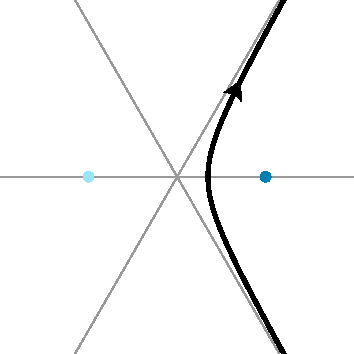
\includegraphics{figures/u_contour_3.pdf} \\[1em]
{\small The contour $\Gamma$ in the $u$ plane.}
\end{center}
With the substitution $t = 2uy^{1/2}$, we can rewrite the Airy integral as
\[ \Ai(y) = y^{1/2}\;\frac{1}{\pi i} \int_{y^{-1/2} \Gamma} \exp\left[\tfrac{2}{3}y^{3/2} \left(4u^3 - 3u\right)\right]\,du. \]
We have rescaled the contour by a factor of two, but it still approaches $\infty$ in the desired way. Note that $4u^3 - 3u$ is the third Chebyshev polynomial.

By considering other Chebyshev polynomials, we can situate the Airy function within the family of {\em Airy-Lucas functions}, so we will go straight to the general case. However, since the Airy function is a classic example in the study of Borel summation and resurgence, it may be useful to see it on its own. For this reason, in Appendix~\ref{airy-appendix} we give a detailed treatment of the Airy function, specializing the general argument of all Airy-Lucas functions.

\subsection{Airy--Lucas}
The Airy-Lucas equation is
\begin{equation}\label{eqn:airy-lucas}
\left[\big(\tfrac{\partial}{\partial y}\big)^2 - (m-1) y^{-1} \tfrac{\partial}{\partial y} - y^{n-2}\right] \psi = 0
\end{equation}
with $n \in \{3, 4, 5, \ldots\}$ and $m \in \{1, 2, \ldots, n-1\}$. A few solutions are given by the Airy-Lucas functions~\cite[equation~3.6]{charbonnier22}
\[ \widehat{\Ai}^{(k)}_{n, m-1}(y) = \left\{\begin{array}{ll}1 & j \text{ even} \\ i & j \text{ odd}\end{array}\right\} \frac{y^{m/2}}{\pi} \int_{\Lambda^{(j)}} \exp\left[\tfrac{2}{n} y^{n/2}\,T_n(u)\right]\,U_{m-1}(u)\,du, \]
where $\Lambda_{j}$ is the Lefschetz thimble through $u = \cos\big(\tfrac{j}{n}\pi\big)$ (see Figure \ref{fig:thimble_n_5}).

\begin{figure}[h]
    \centering
   % \includegraphics{}
    \caption{Integration contour $\Lambda_j$ for the Airy--Lucas function with $n=5$.}
    \label{fig:thimble_n_5}
\end{figure}


\subsubsection{Rewriting as a modified Bessel $\frac{m}{n}$ equation}
We can distill the most interesting parts of the Airy-Lucas function by writing
\[ \widehat{\Ai}^{(k)}_{n, m-1}(y) = \textcolor{magenta}{\text{const.}}\,y^{{m/2}}\,K\big(\tfrac{2}{n} y^{n/2}\big), \]
where
\begin{equation}\label{integral:mod-bessel-rational-AL}
K(z) = \textcolor{magenta}{\text{const.}} \int_{z^{-{1/n}}\Lambda^{(k)}} \exp\left[z T_n(u)\right]\,U_{m-1}(u)\,du.
\end{equation}
Saying that $\widehat{\Ai}^{(k)}_{n, m-1}$ satisfies the Airy-Lucas equation is equivalent to saying that $K$ satisfies the modified Bessel $\frac{m}{n}$ equation
\begin{equation}\label{eqn:mod-bessel-AL}
\left[z^2 \big(\tfrac{\partial}{\partial z}\big)^2 + z \tfrac{\partial}{\partial z} - \big[\big(\tfrac{m}{n} \big)^2 + z^2\big]\right] K = 0.
\end{equation}
In fact, as we will see in Section~\ref{contour-argument-AL}, $K$ is the modified Bessel function $K_{{m/n}}$.

Let's put equation~\eqref{eqn:mod-bessel-AL} in the form \eqref{eqn:standard ODE}:
\begin{equation}\label{eqn:reg-mod-bessel-AL}
\left[ \big[ \big(\tfrac{\partial}{\partial z}\big)^2 - 1 \big] + z^{-1} \tfrac{\partial}{\partial z} - \big({\tfrac{m}{n}}\big)^2 z^{-2} \right] K = 0.
\end{equation}

\subsubsection{Asymptotic analysis}\label{sec:asympt-AL}

From the general theory of ODE of Poincar\'e rank $1$, we know that the space of trans-series solutions of ~\eqref{eqn:reg-mod-bessel-AL} has a basis of trans-monomials
\[ \{ e^{-\alpha z} z^{-\tau_\alpha}\,\series{W}_\alpha \mid \alpha^2 - 1 = 0 \} \]
where the $\series{W}_\alpha\in\C\llbracket z^{-1} \rrbracket$ are formal power series in $z^{-1}$ and $\tau_\alpha=1/2$. From equations 10.40.2 and 10.17.1 of \cite{dlmf}, we learn that $K(z) \sim \left(\tfrac{\pi}{2}\right)^{1/2} e^{-z} z^{-1/2}\,\series{W}_1$, with
\begin{equation}\label{bessel-asymp-AL}
\series{W}_1 = 1 - \frac{(\tfrac{1}{2}-\tfrac{m}{n})_1 (\tfrac{1}{2}+\frac{m}{n})_1}{2^1 \cdot 1!}\;z^{-1} + \frac{(\tfrac{1}{2}-\tfrac{m}{n})_2 (\tfrac{1}{2}+\tfrac{m}{n})_2}{2^2 \cdot 2!}\;z^{-2} - \frac{(\tfrac{1}{2}+\tfrac{m}{n})_3 (\tfrac{1}{2}+\tfrac{m}{n})_3}{2^3 \cdot 3!}\;z^{-3} + \ldots
\end{equation}

The holomorphic analysis in Section~\ref{big-idea} will give us holomorphic solutions
\[ \{ e^{-\alpha z} z^{-\tau_\alpha}\,W_\alpha \mid \alpha^2 - 1 = 0 \}, \]
which seem analogous to the trans-monomials above. Borel summation makes the analogy precise. We will see in Section~\ref{bessel-regularity-AL} that each $z^{-\tau_\alpha}\,W_\alpha$ is proportional to the Borel sum of $z^{-\tau_\alpha}\,\series{W}_\alpha$. This is an evidence of Theorem~\ref{thm1-dim}.
%\subsection{Going to the spatial domain}\label{spatial-AL}
\subsubsection{The big idea}\label{big-idea}
We're going to look for functions $v_\alpha$ whose Laplace transforms $\laplace_{\zeta, \alpha} v_\alpha$ satisfy equation~\eqref{eqn:reg-mod-bessel-AL}. We'll succeed when $\alpha^2 - 1 = 0$, and we'll see that $K$ is a scalar multiple of $\laplace_{\zeta, 1} v_1$.

We can see from Section~\ref{L-int-op} that $\laplace_{\zeta, \alpha} v$ satisfies the differential equation~\eqref{eqn:reg-mod-bessel-AL} if and only if $v$ satisfies the integral equation
\begin{equation}\label{int-eq:spatial-mod-bessel-AL}
\left[ \big[ \zeta^2 - 1 \big] - \fracderiv{-1}{\zeta}{\alpha} \circ \zeta - \big(\tfrac{m}{n}\big)^2 \fracderiv{-2}{\zeta}{\alpha} \right] v = 0.
\end{equation}
It's tempting to differentiate both sides of this equation until we get
\begin{equation}\label{diff-eq:spatial-mod-bessel-AL}
\left[ \big(\tfrac{\partial}{\partial \zeta}\big)^2 \circ \big[ \zeta^2 - 1 \big] - \tfrac{\partial}{\partial \zeta} \circ \zeta - \big(\tfrac{m}{n}\big)^2 \right] v = 0,
\end{equation}
which is easier to solve. Unfortunately, a solution of equation~\eqref{diff-eq:spatial-mod-bessel-AL} won't satisfy equation~\eqref{int-eq:spatial-mod-bessel-AL} in general. However, as we learned in Section~\ref{shifting}, a solution of equation~\eqref{diff-eq:spatial-mod-bessel-AL} {\em will} satisfy equation~\eqref{int-eq:spatial-mod-bessel-AL} if it's slight and locally integrable at $\zeta = \alpha$.

This is great news, because equation~\eqref{diff-eq:spatial-mod-bessel-AL} has a regular singularity at each root of $\zeta^2 - 1$, and the Frobenius method often gives a slight solution at each regular singular point. We can see the regular singularities by moving the derivatives to the right:
\[ \left[ (\zeta^2 - 1) \big(\tfrac{\partial}{\partial \zeta}\big)^2 + 3\zeta \tfrac{\partial}{\partial \zeta} + \big[ 1 - \big(\tfrac{m}{n}\big)^2 \big] \right] v = 0. \]

In Sections \ref{pos-root-AL}\,--\,\ref{neg-root-AL}, we'll see this approach succeed. For each root $\alpha$, we'll find a solution $v_\alpha$ of equation~\eqref{diff-eq:spatial-mod-bessel-AL} which is slight and locally integrable at $\zeta = \alpha$. We know the function $\laplace_{\zeta, \alpha} v_\alpha$ will satisfy equation~\eqref{eqn:reg-mod-bessel-AL}, and we can even find its asymptotics from the order $\tau_\alpha$ of $v_\alpha$. We learned in Section~\ref{translation} that
\[ \laplace_{\zeta, \alpha} v_\alpha = e^{-\alpha z} V_\alpha \]
where $V_\alpha = \laplace_{\zeta_\alpha, 0} v_\alpha$ and $\zeta = \alpha + \zeta_\alpha$. We can see from Section~\ref{reg-decay} that $V_\alpha$ is asymptotic to a scalar multiple of $z^{-1 - \tau_\alpha}$ at $z = \infty$, so the further decomposition
\[ \laplace_{\zeta, \alpha} v_\alpha = e^{-\alpha z} z^{-\tau_\alpha} W_\alpha, \]
makes $W_\alpha$ is asymptotic to a scalar multiple of $z^{-1}$ at $z = \infty$.
%\color{Peru}
%\begin{align*}
%\left[ \big(\tfrac{\partial}{\partial \zeta}\big)^2 \circ (\zeta - 1)(\zeta + 1) - \tfrac{\partial}{\partial \zeta} \circ \zeta - \big(\tfrac{1}{3}\big)^2 \right] v & = 0
%\end{align*}
%\color{Sienna}
%\begin{align*}
%\left[ \big[ 2 + 2(2\zeta) \tfrac{\partial}{\partial \zeta} + (\zeta^2 - 1) \big(\tfrac{\partial}{\partial \zeta}\big)^2 \big] - \big[ 1 + \zeta \tfrac{\partial}{\partial \zeta} \big] - \big(\tfrac{1}{3}\big)^2 \right] v & = 0 \\
%\left[ (\zeta^2 - 1) \big(\tfrac{\partial}{\partial \zeta}\big)^2 + 3\zeta \tfrac{\partial}{\partial \zeta} + \big[ 1 - \big(\tfrac{1}{3}\big)^2 \big] \right] v & = 0 \\
%\left[ (\zeta - 1)(\zeta + 1) \big(\tfrac{\partial}{\partial \zeta}\big)^2 + 3\zeta \tfrac{\partial}{\partial \zeta} + \big[ 1 - \big(\tfrac{1}{3}\big)^2 \big] \right] v & = 0
%\end{align*}
%\color{black}
%%In terms of the coordinate $\zeta_\alpha$ with $\zeta = \alpha + \zeta_\alpha$, this equation is written
%%\begin{equation}\label{eqn:centered-mod-bessel}
%%\[ \left[ \big[ \zeta_\alpha (\zeta_\alpha + 2\alpha) + \alpha^2 - 1 \big] + \fracderiv{-1}{\zeta_\alpha}{0} \circ \big[ \zeta_\alpha + \alpha \big] - \big(\tfrac{1}{3}\big)^2 \fracderiv{-2}{\zeta_\alpha}{0} \right] w = 0. \]
%%\end{equation}
\subsubsection{Focus on $\zeta = 1$}\label{pos-root-AL}
Let's find a solution of equation~\eqref{diff-eq:spatial-mod-bessel-AL} which is slight and locally integrable at $\zeta = 1$. Define a new coordinate $\zeta_1$ on $\C$ so that $\zeta = 1 + \zeta_1$. In this coordinate, equation~\eqref{diff-eq:spatial-mod-bessel-AL} looks like
\begin{equation}\label{diff-eq:spatial-mod-bessel-pos-AL}
\left[\zeta_1(2 + \zeta_1) \big(\tfrac{\partial}{\partial \zeta_1}\big)^2 + 3(1 + \zeta_1) \tfrac{\partial}{\partial \zeta_1} + \big[1 - \big(\tfrac{m}{n}\big)^2\big]\right] v = 0.
\end{equation}
With another change of coordinate, given by $\zeta_1 = -2\xi_1$, we can rewrite equation~\eqref{diff-eq:spatial-mod-bessel-AL} as the hypergeometric equation
\begin{equation}\label{diff-eq:hypergeom-pos-AL}
\left[\xi_1 (1 - \xi_1) \big(\tfrac{\partial}{\partial \xi_1}\big)^2 + 3(\tfrac{1}{2} - \xi_1) \tfrac{\partial}{\partial \xi_1} - \big[1 - \big(\tfrac{m}{n}\big)^2\big]\right] v = 0.
\end{equation}
Looking through the twenty-four expressions for Kummer's six solutions, we find one \cite[formula~15.10.12]{dlmf} which is manifestly slight and locally integrable at $\xi_1 = 0$:
\begin{alignat*}{2}
v_1 &=\;& \hphantom{-i\sqrt{2}}\,\xi_1^{-1/2} & {}_2F_1\big(\tfrac{1}{2}-\tfrac{m}{n}, \tfrac{1}{2}+\tfrac{m}{n}; \tfrac{1}{2}; \xi_1\big) \\
&=\;& -i\sqrt{2}\,\zeta_1^{-1/2} & {}_2F_1\big(\tfrac{1}{2}-\tfrac{m}{n}, \tfrac{1}{2}+\tfrac{m}{n}; \tfrac{1}{2}; -\tfrac{1}{2}\zeta_1\big)
\end{alignat*}
From the argument in Section~\ref{big-idea}, we know that $\laplace_{\zeta, 1} v_1$ satisfies equation~\eqref{eqn:mod-bessel-AL}, and can be written as $e^{-z} V_1$, where $V_1 = \laplace_{\zeta_1, 0} v_1$. Since $v_1$ has order $-1/2$, the decomposition $V_1 = z^{-1/2} W_1$ makes $W_1$ asymptotic to a scalar multiple of $1+O(z^{-1})$ at $z = \infty$.
\subsubsection{Focus on $\zeta = -1$}\label{neg-root-AL}
Let's find a solution of equation~\eqref{diff-eq:spatial-mod-bessel-AL} which is slight and locally integrable at $\zeta = -1$. In the rescaled coordinate from Section~\ref{pos-root-AL}, this is the point $\xi_1 = 1$. Looking again through Kummer's table of solutions, we find another expression \cite[formula~15.10.14]{dlmf} which is manifestly slight and locally integrable at $\xi_1 = 1$:
\begin{alignat*}{2}
v_{-1} &=\;& (1-\xi_1)^{-1/2} & {}_2F_1\big(\tfrac{1}{2}-\tfrac{m}{n}, \tfrac{1}{2}+\tfrac{m}{n}; \tfrac{1}{2}; 1-\xi_1\big) \\
&=\;& \sqrt{2}\,\zeta_{-1}^{-1/2} & {}_2F_1\big(\tfrac{1}{2}-\tfrac{m}{n}, \tfrac{1}{2}+\tfrac{m}{n}; \tfrac{1}{2}; \tfrac{1}{2}\zeta_{-1}\big)
\end{alignat*}
where $\zeta_{-1}$ is the coordinate with $\zeta = -1 + \zeta_{-1}$. From the argument in Section~\ref{big-idea}, we know that $\laplace_{\zeta, -1} v_{-1}$ satisfies equation~\eqref{eqn:mod-bessel-AL}, and can be written as $e^z V_{-1}$, where $V_{-1} = \laplace_{\zeta_{-1}, 0} v_{-1}$. Since $v_{-1}$, like our other solution, has order $-1/2$, the same decomposition $V_{-1} = z^{-1/2} W_{-1}$ makes $W_{-1}$ asymptotic to a scalar multiple of $1+O(z^{-1})$ at $z = \infty$.

In this example, $v_1$ and $v_{-1}$ happen to be related by a symmetry: the M\"{o}bius transformation that pulls $\zeta$ back to $-\zeta$. Kummer's solutions typically come from six different hypergeometric equations, which are related by the M\"{o}bius transformations that permute their singularities. In our case, though, exchanging $1$ with $-1$ keeps equation~\eqref{diff-eq:spatial-mod-bessel-AL} the same.
\subsubsection{Abstract argument for Borel regularity}\label{bessel-regularity-AL}
The analysis in Sections~\ref{big-idea}--\ref{neg-root-AL} picks out a frame in the space of analytic solutions of~\eqref{eqn:reg-mod-bessel-AL}. The frame is generated by solutions of the form $\laplace_{\zeta, 1} v_1$ and $\laplace_{\zeta, -1} v_{-1}$, with $v_\alpha \in \zeta_\alpha^{-1/2} + o\big(\zeta_\alpha^{-1/2}\big)$.
\color{DarkTurquoise}
\begin{quote}
We get $v_\alpha$ from the existence result in Section~\ref{borel_reg-ODE}, which gives $v_\alpha = \zeta^{\tau-1} + v_\alpha'$ with $\tau \in (0, \infty)$ and $v_\alpha' \in \holoL{\infty, 1-\tau-\epsilon}(\Omega)$ for some $\epsilon \in (0, 1]$. Looking back at the definitions of our weighted $L^\infty$ spaces, we can see that
\begin{align*}
v_\alpha' \in \holoL{\infty, 1-\tau-\epsilon}(\Omega) & \Longrightarrow \zeta_\alpha^{1-\tau-\epsilon}\,v_\alpha' \text{ is bounded near } \zeta_\alpha = 0 \\
& \Longrightarrow \zeta_\alpha^\epsilon\,\zeta_\alpha^{1-\tau-\epsilon}\,v_\alpha' \text{ goes to } 0 \text{ as } \zeta_\alpha \text{ goes to } 0 \\
& \Longrightarrow \zeta_\alpha^{1-\tau}\,v_\alpha' \text{ goes to } 0 \text{ as } \zeta_\alpha \text{ goes to } 0 \\
& \Longrightarrow v_\alpha' / \zeta_\alpha^{\tau-1} \text{ goes to } 0 \text{ as } \zeta_\alpha \text{ goes to } 0 \\
& \Longleftrightarrow v_\alpha' \in o\big(\zeta_\alpha^{\tau-1}\big).
\end{align*}
In this case, $\tau = \tfrac{1}{2}$.
\end{quote}
\color{black}

The Poincar\'{e} algorithm, as we saw in Section~\ref{sec:asympt-AL}, picks out a frame in the space of formal trans-series solutions of equation~\eqref{eqn:reg-mod-bessel-AL}. The frame is generated by trans-monomial solutions of the form $e^{-z} z^{-1/2}\,\tilde{W}_1$ and $e^z z^{-1/2}\,\tilde{W}_{-1}$, with $\tilde{W}_\alpha \in \C\llbracket z^{-1} \rrbracket$. We'll now show that if these solutions are Borel-summable, their Borel sums generate the same frame as $\laplace_{\zeta, 1} v_1$ and $\laplace_{\zeta, -1} v_{-1}$.

The Borel transform maps $e^{-\alpha z} z^{-1/2}\,\C\llbracket z^{-1} \rrbracket$ into $\zeta_\alpha^{-1/2}\,\C\llbracket \zeta_\alpha \rrbracket$ (see Section \ref{sec:action_transseries}), and it turns formal trans-monomial solutions of equation~\eqref{eqn:reg-mod-bessel-AL} into formal power series solutions of equation~\eqref{int-eq:spatial-mod-bessel-AL}. Summation sends convergent power series in $\zeta_\alpha^{-1/2}\,\C\llbracket \zeta_\alpha \rrbracket$ into $\zeta_\alpha^{-1/2}+ o\big(\zeta_\alpha^{-1/2}\big)$, and it turns convergent power series that satisfy a given fractional integral equation into holomorphic functions that satisfy the same equation~\textcolor{magenta}{[prove or cite]}. Thus, if $e^{-z} z^{-1/2}\,\tilde{W}_1$ and $e^z z^{-1/2}\,\tilde{W}_{-1}$ are $1$-Gevrey, their Borel transforms sum to solutions of equation~\eqref{int-eq:spatial-mod-bessel-AL}, which lie in $\zeta_\alpha^{-1/2} + o\big(\zeta_\alpha^{-1/2}\big)$ for $\alpha = 1$ and $\alpha = -1$, respectively.

When $\alpha$ is $1$ or $-1$, equation~\eqref{int-eq:spatial-mod-bessel-AL} becomes the kind of singular integral equation discussed in Section~\ref{borel_reg-ODE}. It therefore has exactly one solution in $\zeta_\alpha^{-1/2} + o\big(\zeta_\alpha^{-1/2}\big)$, up to scaling. That means $\borel\big[ e^{-\alpha z} z^{-1/2}\,\tilde{W}_\alpha \big]$ must sum to a scalar multiple of $v_\alpha$. Thus, if $e^{-\alpha z} z^{-1/2}\,\tilde{W}_\alpha$ is Borel-summable, its Borel sum is a scalar multiple of $\laplace_{\zeta, \alpha} v_\alpha$.

\subsubsection{Confirmation of Borel regularity}\label{confirmation-borel-regularity}
We can confirm the conclusion of Section~\ref{bessel-regularity-AL} using our explicit expressions for the formal power series $\tilde{W}_\alpha$ and the functions $v_\alpha$. We found in Section~\ref{sec:asympt-AL} that
\begin{align*}
\tilde{W}_1 & = \sum_{k = 0}^{\infty} \frac{\left(\tfrac{1}{2}-\tfrac{m}{n}\right)_k \left(\tfrac{1}{2}+\tfrac{m}{n}\right)_k}{k!} \left(-\frac{1}{2}\right)^k z^{-k} \\
\tilde{W}_{-1} & = \sum_{k = 0}^{\infty} \frac{\left(\tfrac{1}{2}-\tfrac{m}{n}\right)_k \left(\tfrac{1}{2}+\tfrac{m}{n}\right)_k}{k!} \left(\frac{1}{2}\right)^k z^{-k}.
\end{align*}
Computing
\begin{align*}
\borel_\zeta \big[ e^{-z} z^{-1/2}\,\tilde{W}_1 \big] & = \borel_\zeta \left[ e^{-z} \sum_{k = 0}^{\infty} \frac{\left(\tfrac{1}{2}-\tfrac{m}{n}\right)_k \left(\tfrac{1}{2}+\tfrac{m}{n}\right)_k}{k!} \left(-\frac{1}{2}\right)^k z^{-k-\frac{1}{2}} \right] \\
& = \sum_{k = 0}^{\infty} \frac{\left(\tfrac{1}{2}-\tfrac{m}{n}\right)_k \left(\tfrac{1}{2}+\tfrac{m}{n}\right)_k}{k!} \left(-\frac{1}{2}\right)^k \frac{\zeta_1^{k-\frac{1}{2}}}{\Gamma\big(k+\frac{1}{2}\big)} \\
& = \sum_{k = 0}^{\infty} \frac{\left(\tfrac{1}{2}-\tfrac{m}{n}\right)_k \left(\tfrac{1}{2}+\tfrac{m}{n}\right)_k}{k!} \left(-\frac{1}{2}\right)^k \frac{\zeta_1^{k-\frac{1}{2}}}{\Gamma\big(\frac{1}{2}\big) \left(\frac{1}{2}\right)_k} \\
& = \frac{\zeta_1^{-\frac{1}{2}}}{\Gamma\big(\frac{1}{2}\big)} \sum_{k = 0}^{\infty} \frac{\left(\tfrac{1}{2}-\tfrac{m}{n}\right)_k \left(\tfrac{1}{2}+\tfrac{m}{n}\right)_k}{\left(\frac{1}{2}\right)_k} \left(-\frac{1}{2}\right)^k \frac{\zeta_1^k}{k!},
\end{align*}
we see that $\borel\big[ e^{-z} z^{-1/2}\,\tilde{W}_1 \big]$ sums to
\[ \tfrac{1}{\Gamma(1/2)}\,\zeta_1^{-1/2}\,{}_2F_1\big(\tfrac{1}{2}-\tfrac{m}{n}, \tfrac{1}{2}+\tfrac{m}{n}; \tfrac{1}{2}; -\tfrac{1}{2}\zeta_1\big). \]
Looking back at Section~\ref{pos-root-AL}, we recognize this as a scalar multiple of $v_1$.


Through a similar calculation, we see that $\borel\big[ e^z z^{-1/2}\,\tilde{W}_{-1} \big]$ sums to
\[ \tfrac{1}{\Gamma(1/2)}\,\zeta_{-1}^{-1/2}\,{}_2F_1\big(\tfrac{1}{2}-\tfrac{m}{n}, \tfrac{1}{2}+\tfrac{m}{n}; \tfrac{1}{2}; \tfrac{1}{2}\zeta_{-1}\big). \]
Looking back at Section~\ref{neg-root-AL}, we recognize this as a scalar multiple of $v_{-1}$.



\subsubsection{Thimble projection technique for Airy-Lucas functions}\label{contour-argument-AL}
\textcolor{orange}{[\textbf{New phrasing for rewrite:} The critical point splits the thimble $\Lambda$ into two pieces: the {\em incoming} branch, where the orientation of the thimble runs toward the critical point, and the {\em outgoing} branch, where the orientation points away.]}

We can recast integral~\eqref{integral:mod-bessel-rational-AL} into the $\zeta$ plane by setting $\textcolor{magenta}{-\zeta} = T_n(u)$, which implies that $-d\zeta = n U_{n-1}(u)\,du$. Projecting $z^{-1/n} \Lambda^{(k)}$ to a contour $\gamma_z$ in the $\zeta$ plane and choosing the branch of $u$ that lifts $\gamma_z$ back to $z^{-1/n} \Lambda^{(k)}$, we get \textcolor{magenta}{[sign flipped]} \textcolor{DarkCyan}{[see identity in \texttt{cyl-resurgence.tex}]}
\begin{align*}%%\label{integral:mod-bessel-rational-zeta}
K_{m/n}(z) & = \frac{n}{2 \sinh\big(\tfrac{m}{n}\,i\pi\big)} \int_{z^{-\textcolor{DarkCyan}{1/n}}\Lambda^{(k)}} \exp\left[z T_n(u)\right]\,U_{m-1}(u)\,du \\
& = -\frac{1}{2  \sinh\big(\tfrac{m}{n}\,i\pi\big)} \int_{\gamma_z} e^{-z\zeta}\,\frac{U_{m-1}(u)}{U_{n-1}(u)}\,d\zeta %\\
%& = -\frac{1}{2\,\tfrac{n}{m} \sinh\big(\tfrac{m}{n}\,i\pi\big)} \int_{\gamma_z} e^{-z\zeta}\,F(1 - \tfrac{m}{n}, 1 + \tfrac{m}{n}, \tfrac{3}{2}, \tfrac{1}{2} \pm \tfrac{1}{2}\zeta)\,d\zeta.
\end{align*}


For $z \in (0, \infty)$, the contour $\gamma_z$ runs \textcolor{magenta}{counterclockwise} around $[1, \infty)$, as shown below\textcolor{DarkCyan}{, so we have to choose the negative sign above (?)}. Let's assume $z \in (0, \infty)$ for the rest of the section. \textcolor{magenta}{[Our conclusions should probably hold whenever $\operatorname{Re}(z) > 0$.]}


\begin{center}
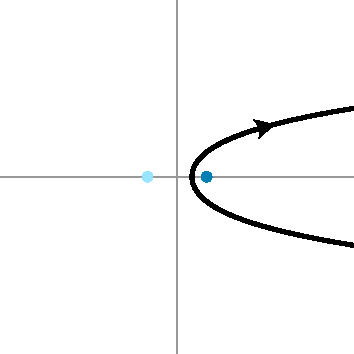
\includegraphics{figures/zeta_contour_3.pdf} \\[1em]
{\small The contour $\gamma_1$ \textcolor{magenta}{[reversed]} in the $\zeta$ plane.}
\end{center}

Now we observe, that by properties of Chebyshev polynomials the integrand can be written as an explicit function of $\zeta$: 

\begin{align*}
    \frac{U_{m-1}(\cos(\phi))}{U_{n-1}(\cos(\phi))}&=\frac{\sin(m\phi)}{\sin(\phi)}\frac{\sin(\phi)}{\sin(n \phi)}\\
    &=\frac{\sin(m\phi)}{\sin(n \phi)}\\
    &=\frac{m}{n}\,\, {}_2F_1\left(\frac{1}{2}-\frac{m}{2n},\frac{1}{2}+\frac{m}{2n};\frac{3}{2};\sin^2(n \phi)\right)\\
    &=\frac{m}{n}\,\, {}_2F_1\left(\frac{1}{2}-\frac{m}{2n},\frac{1}{2}+\frac{m}{2n};\frac{3}{2};1-\zeta^2\right) 
\end{align*}
where in the last step we use $-\zeta=T_n(u)=T_n(\cos\phi)=\cos(n\phi)$. Applying identity 15.8.4, 15.8.27 and 15.8.28 from \cite{dlmf}, 

\begin{align*}
    &{}_2F_1\left(\frac{1}{2}-\frac{m}{2n},\frac{1}{2}+\frac{m}{2n};\frac{3}{2};1-\zeta^2\right)=\\
    &\qquad = \frac{\pi}{\Gamma\left(1-\frac{m}{2n}\right)\Gamma\left(1+\frac{m}{2n}\right)} \,\,\, {}_2F_1\left(\frac{1}{2}-\frac{m}{2n},\frac{1}{2}+\frac{m}{2n};\frac{1}{2};\zeta^2\right)+\\
    &\qquad \qquad\qquad - \frac{\pi \zeta}{\Gamma\left(\frac{1}{2}-\frac{m}{2n}\right)\Gamma\left(\frac{1}{2}+\frac{m}{2n}\right)} \,\,\, {}_2F_1\left(1-\frac{m}{2n},1+\frac{m}{2n};\frac{3}{2};\zeta^2\right)\\
    &\qquad ={}_2F_1\left(1-\frac{m}{n},1+\frac{m}{n};\frac{3}{2};\frac{1}{2}-\frac{\zeta}{2}\right)+{}_2F_1\left(1-\frac{m}{n},1+\frac{m}{n};\frac{3}{2};\frac{1}{2}+\frac{\zeta}{2}\right)+\\
    &\qquad\qquad +\frac{1}{2} {}_2F_1\left(1-\frac{m}{n},1+\frac{m}{n};\frac{3}{2};\frac{1}{2}-\frac{\zeta}{2}\right)-\frac{1}{2}{}_2F_1\left(1-\frac{m}{n},1+\frac{m}{n};\frac{3}{2};\frac{1}{2}+\frac{\zeta}{2}\right)\\
    &\qquad =\frac{3}{2} {}_2F_1\left(1-\frac{m}{n},1+\frac{m}{n};\frac{3}{2};\frac{1}{2}-\frac{\zeta}{2}\right)+\frac{1}{2}{}_2F_1\left(1-\frac{m}{n},1+\frac{m}{n};\frac{3}{2};\frac{1}{2}+\frac{\zeta}{2}\right)
\end{align*}
In addition, recall that ${}_2F_1\left(1-\frac{m}{n},1+\frac{m}{n};\frac{3}{2};\frac{1}{2}-\frac{\zeta}{2}\right)$ has a branch cut singularity at $\zeta=-1$ while ${}_2F_1\left(1-\frac{m}{n},1+\frac{m}{n};\frac{3}{2};\frac{1}{2}+\frac{\zeta}{2}\right)$ has a branch cut at $\zeta=1$; hence 

\begin{align*}
    K_{m/n}(z)&=-\frac{m}{4 n\sinh(\tfrac{m}{n}i\pi)}\int_{\gamma_z}e^{-z\zeta} {}_2F_1\left(1-\frac{m}{n},1+\frac{m}{n};\frac{3}{2};\frac{1}{2}+\frac{\zeta}{2}\right) d\zeta\\
    &=-\frac{1}{2}\int_{1}^{+\infty}e^{-z\zeta} \left(-\frac{1}{2}+\frac{\zeta}{2}\right)^{-1/2} {}_2F_1\left(\frac{1}{2}-\frac{m}{n},\frac{1}{2}+\frac{m}{n};\frac{1}{2};\frac{1}{2}-\frac{\zeta}{2}\right) d\zeta
\end{align*}

where in the second step we use the analytic continuation of the hypergeometric function (equation 15.2.3 in \cite{dlmf}). 

Finally, comparing this expression for $K_{m/n}$ with the expression for $v_1$ computed in Section \ref{pos-root} we notice that 
\begin{align*}
    K_{m/n}(z)=\frac{i}{2}\laplace_{\zeta,1}v_1 .
\end{align*}

\subsubsection{A flavour of resurgence: the Stokes phenomena in the position domain}\label{resurgence-AL}

In the previous sections, we have seen how to compute the Borel transform of a formal frame of solutions of the modified Bessel equation with parameter $m/n$ (\S\ref{confirmation-borel-regularity}) or equivalently of the asymptotic expansion of thimble integrals $K_{m/n}$ (\S\ref{contour-argument-AL}). Up to a constant, in both cases we find 

\begin{align*}
    v_1(\zeta)= i \left(-\frac{1}{2}+\frac{\zeta}{2}\right)^{-1/2} {}_2F_1\left(\frac{1}{2}-\frac{m}{n},\frac{1}{2}+\frac{m}{n};\frac{1}{2};\frac{1}{2}-\frac{\zeta}{2}\right)
\end{align*}

which has a fractional power singularity at $\zeta=1$. In addition, notice that the hypergeometric function ${}_2F_1\left(\frac{1}{2}-\frac{m}{n},\frac{1}{2}+\frac{m}{n};\frac{1}{2};\frac{1}{2}-\frac{\zeta}{2}\right)$ is convergent at $\zeta=1$ therefore $v_1$ has the typical form of a \textit{singularity} in the formalism of Ecalle's resurgent functions. More precisely, we can consider ${}_2F_1\left(\frac{1}{2}-\frac{m}{n},\frac{1}{2}+\frac{m}{n};\frac{1}{2};\frac{1}{2}-\frac{\zeta}{2}\right)$ as a new germ of holomorphic function, which has a branch cut singularity at $\zeta=-1$. Using equation \cite[15.2.3]{dlmf}, we can compute the analytic continuation of this germ at $\zeta=-1$: 

\begin{align*}
&{}_2F_1\left(\frac{1}{2}-\frac{m}{n},\frac{1}{2}+\frac{m}{n};\frac{1}{2};-\frac{\zeta_1}{2}+i\varepsilon\right)-{}_2F_1\left(\frac{1}{2}-\frac{m}{n},\frac{1}{2}+\frac{m}{n};\frac{1}{2};-\frac{\zeta_1}{2}-i\varepsilon\right)=\\
&=\frac{2\pi i}{\Gamma\big(\tfrac{1}{2}-\tfrac{m}{n}\big)\Gamma\big(\tfrac{1}{2}+\tfrac{m}{n}\big)} \left(-\frac{\zeta_{-1}}{2}\right)^{-1/2} {}_2F_1\left(\frac{m}{n},-\frac{m}{n};\frac{1}{2};\frac{\zeta_{-1}}{2}\right) \\
&=2 i\cos(\pi m/n) \left(-\frac{\zeta_{-1}}{2}\right)^{-1/2} {}_2F_1\left(\frac{m}{n},-\frac{m}{n};\frac{1}{2};\frac{\zeta_{-1}}{2}\right) \\
&=2\cos(\pi m/n) \left(\frac{\zeta_{-1}}{2}\right)^{-1/2} {}_2F_1\left(\frac{m}{n},-\frac{m}{n};\frac{1}{2};\frac{\zeta_{-1}}{2}\right) \\
&=2\cos(\pi m/n)\, \left(\frac{\zeta_{-1}}{2}\right)^{-1/2} \left(-\frac{\zeta_{1}}{2}\right)^{1/2}\, {}_2F_1\left(\frac{1}{2}-\frac{m}{n},\frac{1}{2}+\frac{m}{n};\frac{1}{2};\frac{\zeta_{-1}}{2}\right)
\end{align*}

Hence, we deduce  
\begin{equation}\label{resurgent-relation-1}
    v_1(\zeta+1+i\varepsilon)-v_1(\zeta+1+i\varepsilon)=2i \cos(\pi m/n)  v_{-1}(\zeta)
\end{equation}

namely, that the germ of the singularity at $\zeta=1$ knows about the germ of the singularity at $\zeta=-1$. This is an instance of \textit{resurgent functions}, introduced by Ecalle in \cite{EcalleI}\cite{EcalleII}\cite{EcalleIII}\footnote{If the reader is interesting in resurgence, it may be useful to look at the following review \cite{diverg-resurg-i}\cite{Dorigoni}\cite{aniceto2019primer}.}. Although we will not discuss more about resurgence, we would like to point out that among the great advantages of resurgence (for instance compared to Borel summability) there are the \textit{formalism of singularities} and the \textit{Alien calculus} which allow to understand the Stokes phenomena working in the position domain. The same phenomena were described by Berry and Howls \cite{berry1991hyperasymptotics} who noticed that divergent asymptotic expansions of thimble integrals encode the contribution of other critical values.

We can repeat the same reasoning with $v_{-1}$:

\begin{align*}
    v_{-1}(\zeta)=  \left(\frac{1}{2}+\frac{\zeta}{2}\right)^{-1/2} {}_2F_1\left(\frac{1}{2}-\frac{m}{n},\frac{1}{2}+\frac{m}{n};\frac{1}{2};\frac{1}{2}+\frac{\zeta}{2}\right)
\end{align*}

and ${}_2F_1\left(\frac{1}{2}-\frac{m}{n},\frac{1}{2}+\frac{m}{n};\frac{1}{2};\frac{1}{2}+\frac{\zeta}{2}\right)$ is singular at $\zeta=1$. Hence

\begin{align*}
&{}_2F_1\left(\frac{1}{2}-\frac{m}{n},\frac{1}{2}+\frac{m}{n};\frac{1}{2};\frac{\zeta_{-1}}{2}+i\varepsilon\right)-{}_2F_1\left(\frac{1}{2}-\frac{m}{n},\frac{1}{2}+\frac{m}{n};\frac{1}{2};\frac{\zeta_{-1}}{2}-i\varepsilon\right)=\\
&=\frac{2\pi i}{\Gamma\big(\tfrac{1}{2}-\tfrac{m}{n}\big)\Gamma\big(\tfrac{1}{2}+\tfrac{m}{n}\big)} \left(\frac{\zeta_{1}}{2}\right)^{-1/2} {}_2F_1\left(\frac{m}{n},-\frac{m}{n};\frac{1}{2};-\frac{\zeta_{1}}{2}\right) \\
&=2 i\cos(\pi m/n) \left(\frac{\zeta_{1}}{2}\right)^{-1/2} {}_2F_1\left(\frac{m}{n},-\frac{m}{n};\frac{1}{2};-\frac{\zeta_{1}}{2}\right) \\
&=2i \cos(\pi m/n)\, \left(\frac{\zeta_{1}}{2}\right)^{-1/2} \left(\frac{\zeta_{-1}}{2}\right)^{1/2}\, {}_2F_1\left(\frac{1}{2}-\frac{m}{n},\frac{1}{2}+\frac{m}{n};\frac{1}{2};-\frac{\zeta_{1}}{2}\right)
\end{align*}

and the analogue of \eqref{resurgent-relation-1} is 
\begin{equation}\label{resurgent-realtion-2}
    v_{-1}(\zeta-1+i\varepsilon)-v_{-1}(\zeta-1-i\varepsilon)= -2i\cos(\pi m/n) v_1(\zeta).
\end{equation}


Equations \eqref{resurgent-relation-1} and \eqref{resurgent-realtion-2} are a manifestation of the Stokes phenomena, already in the position domain. Indeed, when we start varying the contour of integration for the Laplace transform, we know that $\laplace_{\zeta,1}^\pi$ and $\laplace_{\zeta,-1}^0$ are not well defined because the contour hits the other singularity (respectively at $\zeta=-1$ and $\zeta=1$). The Stokes phenomenon consists of comparing the Laplace transform below and above the critical direction and it quantifies the jump as a constant (the so-called Stokes constant) times another function. In our example:

\begin{align*}
    \laplace_{\zeta,1}^{\pi+\varepsilon} v_1-\laplace_{\zeta,1}^{\pi-\varepsilon} v_1 & = 2 i \cos(\pi m/n) \, e^{-z}\, \laplace_{\zeta,-1}^{\pi} v_{-1} \\
    \laplace_{\zeta,-1}^{\varepsilon} v_{-1}-\laplace_{\zeta,-1}^{-\varepsilon} v_{-1} & = - 2 i \cos(\pi m/n)  \, e^z \, \laplace_{\zeta,1} v_{1} 
\end{align*}

thus the Stokes constants are respectively $\pm 2i \cos(\pi m/n)$\footnote{If we think of the Laplace transforms of $v_1$ and $v_{-1}$ as a frame of solutions for the Airy--Lucas differential equation, the equations above define the so-called Stokes matrices for the ODE.}. 

It may be surprising that the Stokes constants depend on $\cos(\pi m/n)$, as the Stokes constants are the intersection number of \textit{dual pair of thimbles}, according to Picard--Lefschetz formula (in particular, they are integers in a suitable normalization), see \cite[Section 5]{pham} and Figure \ref{fig:intersection_thimbles}. However, in the Airy--Lucas example, $f$ is not Morse (unless $n=3$), hence we have to interpret the $\cos(\pi m/n)$ as a consequence of the ambiguity on a lift of a path in the position domain. \textcolor{orange}{ I think we should argue we have the action of the permutation which leaves the base unchanged but gives a } 

\begin{figure}[h]
    \centering
    %\includegraphics{}
    \caption{Graphically, we can describe the Stokes phenomenon by looking at the intersection points of \textit{dual pairs of thimbles}, which differ by a rotation of angle $\pi$. We choose $n=4$ and $n=5$. }
    \label{fig:intersection_thimbles}
\end{figure}




%\textcolor{DarkCyan}{where the sign must be chosen so that $\pm\zeta$ stays in the left half-plane over the whole integration path (?)}.
%For $z \in (0, \infty)$, the contour $\gamma_z$ runs \textcolor{magenta}{counterclockwise} around $[1, \infty)$, as shown below\textcolor{DarkCyan}{, so we have to choose the negative sign above (?)}. Let's assume $z \in (0, \infty)$ for the rest of the section. \textcolor{magenta}{[Our conclusions should probably hold whenever $\operatorname{Re}(z) > 0$.]}


%The integrand is non-meromorphic at $\zeta = 1$. Along the branch cut $\zeta \in [1, \infty)$, its above-minus-below difference is
%\begin{align*}
%& -(2\pi i)\tfrac{n}{2\pi m} \sin(\tfrac{m}{n} \pi)\,(\pm\tfrac{1}{2}\zeta - \tfrac{1}{2})^{-1/2} {}_2F_1(\tfrac{1}{2} - \tfrac{m}{n}, \tfrac{1}{2} + \tfrac{m}{n}, \tfrac{1}{2}, \tfrac{1}{2} \mp \tfrac{1}{2}\zeta) \\
%= & -\tfrac{n}{m} \sinh(\tfrac{m}{n}\,i\pi)\,(\pm\tfrac{1}{2}\zeta - \tfrac{1}{2})^{-1/2} {}_2F_1(\tfrac{1}{2} - \tfrac{m}{n}, \tfrac{1}{2} + \tfrac{m}{n}, \tfrac{1}{2}, \tfrac{1}{2} \mp \tfrac{1}{2}\zeta),
%\end{align*}
%as given\footnote{Note that $\Gamma(\tfrac{3}{2}) \Gamma(\tfrac{1}{2})^{-1} = \tfrac{1}{2}$ and $\big[\Gamma(1 - \tfrac{m}{n})\Gamma(1 + \tfrac{m}{n})\big]^{-1} = \big[\Gamma(1 - \tfrac{m}{n})\,\tfrac{m}{n}\Gamma(\tfrac{m}{n})\big]^{-1} = \tfrac{n}{m\pi} \sin(\tfrac{m}{n} \pi)$.} by equation~15.2.3 from \cite{dlmf}. Hence, $K_{m/n}$ turns out to be the Laplace transform along $(1, \infty)$ of
%\[ \tfrac{1}{2}\,(-\tfrac{1}{2}\zeta - \tfrac{1}{2})^{-1/2} F(\tfrac{1}{2} - \tfrac{m}{n}, \tfrac{1}{2} + \tfrac{m}{n}, \tfrac{1}{2}, \tfrac{1}{2} + \tfrac{1}{2}\zeta). \]
%\color{DarkCyan}
%Guessing the branch of the square root for consistency with the numerically checked result in Section~\ref{contour-argument}, we get
%\[ \tfrac{i}{2}\,(\tfrac{1}{2} + \tfrac{1}{2}\zeta)^{-1/2} F(\tfrac{1}{2} - \tfrac{m}{n}, \tfrac{1}{2} + \tfrac{m}{n}, \tfrac{1}{2}, \tfrac{1}{2} + \tfrac{1}{2}\zeta). \]
%In other words, $K_{m/n} = \tfrac{i}{2} \laplace_{\zeta, -1} v_{-1}$ with
%\[ v_{-1} = \sqrt{2}\,\zeta_{-1}^{-1/2} F(\tfrac{1}{2} - \tfrac{m}{n}, \tfrac{1}{2} + \tfrac{m}{n}, \tfrac{1}{2}, \tfrac{1}{2}\zeta_{-1}), \]
%where $\zeta = -1 + \zeta_{-1}$.
%\color{black}


\subsection{Modified Bessel}

The modified Bessel equation is a generalization of equation~\eqref{eqn:mod-bessel-AL} where $\frac{m}{n}$ is replaced by a complex parameter $\mu$

\begin{equation}\label{eqn:mod-bessel}
\left[z^2 \big(\tfrac{\partial}{\partial z}\big)^2 + z \tfrac{\partial}{\partial z} - \big[\mu^2 + z^2\big]\right] \varphi = 0
\end{equation}

and a basis of solutions is given by the modified Bessel functions (see formulas~10.27.4 and 10.32.12 from \cite{dlmf} \textcolor{red}{10 \cite{watson1922treatise}}) 

\begin{align*}
I_{\mu}(z)&=\frac{1}{2\pi i}\int_{\Omega} e^{z\cosh t - \mu t} dt \\
K_{\mu}(z)&=\frac{\pi}{\sin(\mu \pi)}\cdot \frac{1}{2}[ I_{-\mu}(z) - I_{\mu}(z)]\\
\color{red}K_{\mu}(z)& \color{red}=\int_{-\infty+i\pi/2}^{+\infty+\pi i/2} e^{-\cosh(t)+\mu t} dt \text{  for } -1<\Re \mu<1
\end{align*} 

where $\Omega$ is a path that comes from $\infty$ along $-i \pi + (0, \infty)$ and goes to $\infty$ along $i \pi + (0, \infty)$ (see Figure \ref{fig:Omega_path}).

\begin{figure}[h]
\center
\begin{tikzpicture}
        \draw[->] (0,2)--(4,2);
        \draw[->] (2,0)--(2,4);
        \draw[red,very thick,->] (4,1.5)--(3,1.5);
        \draw[red,very thick] (3,1.5)--(2,1.5);
        \draw[red,very thick] (4,2.5)--(3,2.5);
        \draw[red,very thick,->] (2,2.5)--(3,2.5);
        \draw[red,very thick] (2,1.5)--(2,2.5);
        \node[red,below, font=\tiny] at (4,1.5) {$\Omega$};
        \node[font=\tiny,left,below] at (1.75,1.5) {$-i\pi$};
        \node[font=\tiny] at (1.8,2.5) {$i\pi$};
\end{tikzpicture}
\caption{The path $\Omega$. }\label{fig:Omega_path}
\end{figure}

On the one hand, this new condition does not really affect the argument we present in Section~\ref{bessel-regularity-AL}, so we briefly state the main results: 

\begin{itemize}
 \item \textbf{Asymptotic analysis}: equation~\eqref{eqn:mod-bessel} admits a basis of formal solutions $K_{\mu}\sim e^{-z} z^{-1/2} \tilde{W}_{\mu, 1}$ and $I_{\mu} \sim e^z z^{-1/2} \tilde{W}_{\mu, 2}$ with 
 \begin{align*}
 \tilde{W}_{\mu,1} &= 1- \frac{\big(\tfrac{1}{2}-\mu\big)\big(\frac{1}{2}+\mu\big)}{2 \cdot 1!} z^{-1} + \frac{\big(\tfrac{1}{2}-\mu\big)_2\big(\frac{1}{2}+\mu\big)_2}{2^2 \cdot 2!} z^{-2} - \frac{\big(\tfrac{1}{2}-\mu\big)_3\big(\frac{1}{2}+\mu\big)_3}{2^3 \cdot 3!} z^{-3}+...\\
 \tilde{W}_{\mu,2} &= 1+\frac{\big(\tfrac{1}{2}-\mu\big)\big(\frac{1}{2}+\mu\big)}{2 \cdot 1!} z^{-1} + \frac{\big(\tfrac{1}{2}-\mu\big)_2\big(\frac{1}{2}+\mu\big)_2}{2^2 \cdot 2!} z^{-2}+ \frac{\big(\tfrac{1}{2}-\mu\big)_3\big(\frac{1}{2}+\mu\big)_3}{2^3 \cdot 3!} z^{-3} + ...
\end{align*}   
 \item  \textbf{Frame of analytic solutions}: there exist two functions $v_{\mu, 1}, v_{\mu, -1}$ such that $\laplace_{\alpha}v_{\mu, \alpha}$ satisfies equation~\eqref{eqn:mod-bessel} and they are explicitly 

\begin{align*}
v_{\mu, 1}&=-i\sqrt{2}\,\zeta_{1}^{-1/2}  {}_2F_1\big(\tfrac{1}{2}-\mu, \tfrac{1}{2}+\mu; \tfrac{1}{2}; -\tfrac{1}{2}\zeta_{1}\big)\\
v_{\mu, -1}&=\sqrt{2}\,\zeta_{-1}^{-1/2}  {}_2F_1\big(\tfrac{1}{2}-\mu, \tfrac{1}{2}+\mu; \tfrac{1}{2}; \tfrac{1}{2}\zeta_{-1}\big)
\end{align*}
\item \textbf{Borel regularity} We can compare the Borel transform of the formal solutions $\tilde{W}_{\mu,\pm1}$ with the analytic solutions $v_{\mu,\pm 1}$. They agree (up to the choice of a constant), hence we have another example where Borel regularity can be checked explicitly. 
\end{itemize}

The thimble projection reasoning we describe in Section~\ref{contour-argument-AL} has to be generalized, as we will discuss in the following Section~\ref{countable-cover}. 



\subsubsection{Lifting to a countable cover}\label{countable-cover}
Formula~\eqref{integral:mod-bessel-rational-AL} expresses the modified Bessel function $K_{m/n}$ as an exponential integral on a finite cover of $\C$. Lifting to a countable cover reveals this formula as a special case of a general integral formula for modified Bessel functions.

Setting $u = \cosh(t/n)$ and recalling that
\begin{align*}
\cosh(n\tau) & := T_n(\cosh(\tau)) \\
\sinh(m\tau) & := U_{m-1}(\cosh(\tau)) \sinh(\tau),
\end{align*}
we can rewrite formula~\eqref{integral:mod-bessel-rational-AL} as \textcolor{magenta}{[switching to the conventional sign for the projection map, so $\Lambda^{(3)}$ now comes from $\infty$ at $-60^\circ$ and goes to $\infty$ at $60^\circ$]}
\begin{align}
\notag K_{m/n}(z) & = \frac{n}{2 \sinh\big(\tfrac{m}{n}\,i\pi\big)} \int_{z^{-\textcolor{DarkCyan}{1/n}}\Lambda^{(k)}} \exp\left[z T_n(u)\right]\,U_{m-1}(u)\,du \\
\notag & = \frac{n}{2 \sinh\big(\tfrac{m}{n}\,i\pi\big)} \int_{\textcolor{magenta}{\Omega}} \exp\left[z \cosh(t)\right]\,U_{m-1}(\cosh(t/n))\,\sinh(t/n)\,d(t/n) \\
\label{integral:mod-bessel-lifted} & = \frac{1}{2 \sinh\big(\tfrac{m}{n}\,i\pi\big)} \int_{\textcolor{magenta}{\Omega}} \exp\left[z \cosh(t)\right]\,\sinh\big(\tfrac{m}{n}\,t\big)\,dt.
\end{align}
For any $\mu \in \C \smallsetminus \Z$, 
\begin{align}
\notag K_\mu(z) & = \frac{\pi}{\sin(\mu \pi)} \cdot \frac{1}{2}\big[ I_{-\mu}(z) - I_\mu(z) \big] \\
\notag & = \frac{1}{2i \sin(\mu \pi)} \int_\Omega \exp\left[z \cosh(t)\right]\,\frac{1}{2}\left[e^{\mu t} - e^{-\mu t}\right]\,dt \\
& \label{int:mod-bessel-gen} = \frac{1}{2 \sinh(\mu\,i\pi)} \int_\Omega \exp\left[z \cosh(t)\right]\,\sinh(\mu t)\,dt,
\end{align}
where $\Omega$ is a path that comes from $\infty$ along $-i \pi + (0, \infty)$ and goes to $\infty$ along $i \pi + (0, \infty)$. The integral converges when $z$ is in the right half-plane. We get formula~\eqref{integral:mod-bessel-lifted} when we choose a rational parameter $\mu = m/n$.

\begin{center}
    \begin{tikzpicture}
        \draw[->] (6,2)--(10,2);
        \draw[->] (8,0)--(8,4);
        \draw[red,thick,->] (10,1.8) .. controls (8,2) .. (10,2.2);
        %\draw[red,thick,->] (10,2)--(9,2);
        %\draw[red,thick] (9,2)--(8.5,2);
        %\draw[red,thick] (10,2)--(9.3,2);
        %\draw[red,thick,->] (8.5,2)--(9.3,2);
        \node[red,below, font=\tiny] at (10,1.8) {$\gamma_z$};
        \node[font=\tiny,below] at (8.5,2) {$1$};
    \end{tikzpicture}
\end{center}

We can now follow Section \ref{contour-argument-AL} to compute the Borel transform of $K_\mu$ as an inverse Laplace transform: let $\zeta=-\cosh(t)$

\begin{align*}
    K_\mu(z)& = -\frac{1}{2 \sinh(\mu\,i\pi)} \int_{\gamma_z} e^{-z \zeta}\,\frac{\sinh(\mu t)}{\sinh(t)}\,d\zeta  & \\
    &=-\frac{\mu}{2 \sinh(\mu\,i\pi)} \int_{\gamma_z} e^{-z \zeta}\, {}_2F_1\left(\frac{1+\mu}{2},\frac{1-\mu}{2};\frac{3}{2};1-\zeta^2\right)\,d\zeta & \cite[15.4.16]{dlmf}
\end{align*}

where $\gamma_z$ is Hankel contour coming from $\infty$ to $1$ and then going back to $\infty$. Using formula \cite[15.8.4]{dlmf}, followed by \cite[15.8.27]{dlmf} and \cite[15.8.28]{dlmf}

\begin{multline*}
     {}_2F_1\left(\frac{1+\mu}{2},\frac{1-\mu}{2};\frac{3}{2};1-\zeta^2\right) = \\
     =\frac{3}{2}\, {}_2F_1\left(1-\mu,1+\mu,\frac{3}{2};\frac{1-\zeta}{2}\right)+\frac{1}{2}\, {}_2F_1\left(1-\mu,1+\mu,\frac{3}{2};\frac{1+\zeta}{2}\right)
\end{multline*}
hence 

\[K_\mu(z)=\frac{\mu\, i}{4 \sin(\mu\pi)} \int_{\gamma_z} e^{-z \zeta}\, {}_2F_1\left(1-\mu,1+\mu;\frac{3}{2};\frac{1+\zeta}{2}\right)\,d\zeta\]

Equation \cite[15.2.3]{dlmf} gives the analytic continuation of hypergeometric functions across the branch cut:

\begin{align}
    K_{\mu}(z)& \label{eqn:K-mu}=-\frac{1}{2}\int_1^\infty e^{-z\zeta} \, \left(\frac{\zeta-1}{2}\right)^{-1/2} \,\, {}_2F_1\left(\frac{1}{2}-\mu, \frac{1}{2}+\mu;\frac{1}{2};\frac{1-\zeta}{2}\right)  d\zeta\\
    &  \notag=-\frac{i}{2}\laplace_{\zeta,1} v_{\mu,1} . 
\end{align}

When $\mu$ goes to $0$, formula~\eqref{int:mod-bessel-gen} becomes
\[ K_0(z) = \frac{1}{2\pi i} \int_\Omega \exp\left[z \cosh(t)\right]\,t\,dt. \]
Choosing $\Omega$ to be the unit-speed path that runs from $\infty$ leftward to $-i\pi$, upward to $i\pi$, and rightward back to $\infty$, we can rewrite this formula as
\begin{align*}
K_0(z) & = \frac{1}{2\pi i} \int_0^\infty \exp\left[-z \cosh(t)\right]\,2\pi i\,dt \\
& = \int_0^\infty \exp\left[-z \cosh(t)\right]\,dt \\
& = \int_1^\infty \exp\left[-z\,\tfrac{1}{2}\left(s + \tfrac{1}{s}\right)\right]\,\frac{ds}{s},
\end{align*}
with $s = e^t$. This is a special case of formula~10.32.9 from \cite{dlmf}. Then equation \eqref{eqn:K-mu} gives

\begin{equation}
    K_0(z)=-\frac{1}{2}\int_1^\infty e^{-z\zeta} \, \left(\frac{\zeta-1}{2}\right)^{-1/2} \,\, {}_2F_1\left(\frac{1}{2}, \frac{1}{2};\frac{1}{2};\frac{1-\zeta}{2}\right)  d\zeta =  \int_1^\infty \frac{e^{-z\zeta}}{\sqrt{\zeta^2-1}} \, d\zeta .
\end{equation}
\textcolor{orange}{[can we use (51) directly? It seems to me that if I try the thimble projection reasoning from the integral expression directly, I'm not able to write $1/\sinh(it)$ as a function of $\zeta$. ]}

\subsection{Higher Airy}

\textcolor{magenta}{[The higher Airy example is not completed and there are still some difficulties in the computations, even for simple examples. Should we remove it?]}

The higher Airy equation is
\begin{equation}\label{eqn:higher-airy}
\left[\big({-}\tfrac{\partial}{\partial y}\big)^{n-1} - y\right] \psi = 0
\end{equation}
with $n \in \{3, 4, 5, \ldots\}$. A few solutions are given by the hyper-Airy functions~\cite{charbonnier22}, equation~3.8

\color{Peru}
With
\begin{align*}
z & = (-1)^{n-1} \tfrac{n-1}{n} y^{n/(n-1)} & w & = (-1)^n (n-1) y^{1/(n-1)} u,
\end{align*}
we have
\begin{align*}
\widetilde{\Ai}^{(k)}_n(y) & = \frac{\exp\big(\pi ik \tfrac{n-2}{n-1}\big)}{2\pi i} \int_{\Lambda^{(j)}} \exp\left[\tfrac{1}{n}w^n - yw\right]\,dw \\
& = \frac{\exp\big(\pi ik \tfrac{n-2}{n-1}\big)}{2\pi i} \int_{\Lambda^{(j)}} \exp\left[\tfrac{1}{n}w \left(w^{n-1} - ny\right)\right]\,dw \\
& = \frac{\exp\big(\pi ik \tfrac{n-2}{n-1}\big)}{2\pi i} \int_{\Lambda^{(j)}} \exp\left[\tfrac{1}{n}w \big((n-1)^{n-1} yu^{n-1} - ny\big)\right]\,dw \\
& = \frac{\exp\big(\pi ik \tfrac{n-2}{n-1}\big)}{2\pi i} \int_{\Lambda^{(j)}} \exp\left[\tfrac{1}{n}yw \big((n-1)^{n-1} u^{n-1} - n\big)\right]\,dw \\
& = \frac{\exp\big(\pi ik \tfrac{n-2}{n-1}\big)}{2\pi i} \int_{\Lambda^{(j)}} \exp\left[(-1)^n \tfrac{n-1}{n} y^{n/(n-1)} u\big((n-1)^{n-1} u^{n-1} - n\big)\right]\,dw \\
& = \frac{\exp\big(\pi ik \tfrac{n-2}{n-1}\big)}{2\pi i} \int_{\Lambda^{(j)}} \exp\left[-z\big((n-1)^{n-1} u^n - nu\big)\right]\,dw \\
& = (-1)^n (n-1) \frac{\exp\big(\pi ik \tfrac{n-2}{n-1}\big)}{2\pi i} y^{1/(n-1)}\int_{\Lambda^{(j)}} \exp\left[-z\big((n-1)^{n-1} u^n - nu\big)\right]\,du \\
& = (-1)^n (n-1) \frac{\exp\left(\pi ik \big(1 - \tfrac{1}{n-1}\big)\right)}{2\pi i} y^{1/(n-1)}\int_{\Lambda^{(j)}} \exp\left[-z\big((n-1)^{n-1} u^n - nu\big)\right]\,du \\
& = (-1)^{n+k} (n-1) \frac{\exp\big({-}\pi i \tfrac{k}{n-1}\big)}{2\pi i} y^{1/(n-1)}\int_{\Lambda^{(j)}} \exp\left[-z\big((n-1)^{n-1} u^n - nu\big)\right]\,du \\
\end{align*}
\color{black}
\[ \widetilde{\Ai}^{(k)}_n(y) = (-1)^{n+k} (n-1) \frac{\exp\big({-}\pi i \tfrac{k}{n-1}\big)}{2\pi i} y^{1/(n-1)}\int_{\Lambda^{(j)}} \exp\left[-z\big((n-1)^{n-1} u^n - nu\big)\right]\,du \\, \]
where $\Lambda^{(k)}$ is the Lefschetz thimble through $u = \cos\big(\tfrac{k}{n}\pi\big)$.
\subsubsection{Rewriting as a \textcolor{magenta}{(???)} equation}
We can distill the most interesting parts of the hyper-Airy function by writing
\[ \widetilde{\Ai}^{(k)}_n(y) = \textcolor{magenta}{\text{const.}}\,y^{1/(n-1)}\,K^{(k)}\left((-1)^n\,\tfrac{n-1}{n}\,y^{n/(n-1)}\right), \]
where
\begin{equation}\label{int_higher-Ariy}
K^{(k)}(z) = \textcolor{magenta}{\text{const.}} \int_{\textcolor{magenta}{\text{const.}(n)} z^{-\textcolor{DarkCyan}{1/n}}\Lambda^{(k)}} \exp\left[-z\big((n-1)^{n-1} u^n - nu\big)\right]\,du.
\end{equation}
Saying that $\widetilde{\Ai}^{(k)}_n$ satisfies the higher Airy equation is equivalent to saying that $K$ satisfies an equation of the form
\begin{equation}\label{eqn:higher-Airy}
\left[ \big[ \big({-}\tfrac{\partial}{\partial z}\big)^{n-1} - 1 \big] - c_n^{(1)} z^{-1} \big({-}\tfrac{\partial}{\partial z}\big)^{n-2} - c_n^{(2)} z^{-2} \big({-}\tfrac{\partial}{\partial z}\big)^{n-3} - \ldots - c_n^{(n-1)} z^{-(n-1)} \right] K^{(k)} = 0.
\end{equation}
The sub-leading coefficients are 
\[ c_n^{(1)} = \frac{n-1}{2}. \]

The later coefficients can be written as\footnote{Many thanks to Peter Taylor for noticing this [\url{https://mathoverflow.net/q/422337/1096}].}
\[ c_n^{(k)} = \frac{b_n^{(k)}}{n^k}\,\frac{\Gamma(n+2)}{\Gamma(n-k)} \]
in terms of the polynomials

\begin{tabular}{llllllllllll}
$b_n^{(2)}$ & = & $\frac{1}{24}$ \\
$b_n^{(3)}$ & = & $\frac{1}{48} n$ \\
$b_n^{(4)}$ & = & $\frac{73}{5760} n^2$ & + & $\frac{1}{1152} n$ & - & $\frac{1}{2880}$ \\
$b_n^{(5)}$ & = & $\frac{11}{1280} n^{3}$ & + & $\frac{1}{768} n^{2}$ & - & $\frac{1}{1920} n$ \\
$b_n^{(6)}$ & = & $\frac{3625}{580608} n^{4}$ & + & $\frac{61}{41472} n^{3}$ & - & $\frac{181}{322560} n^{2}$ & - & $\frac{1}{41472} n$ & + & $\frac{1}{181440}$. 
\end{tabular}

\vspace{5mm}


Searching for 580608 in the OEIS turns up the leading coefficients $\beta^{(k)}$ of these polynomials, which are listed as {\tt A249276} and {\tt A249277}. They're defined by the identity [Yang, ``Approximations for Constant $e$ and Their Applications'']
\[ \frac{1}{e} \left(\frac{n}{n-1}\right)^{n-1} = 1 - \frac{1/2}{n} - \frac{\beta^{(2)}}{n^2} - \frac{\beta^{(3)}}{n^3} - \frac{\beta^{(4)}}{n^4} - \frac{\beta^{(5)}}{n^5} - \ldots, \]
which tells us that
\[ \frac{1}{e} \left(\frac{n}{n-1}\right)^{n-1} = 1 - \frac{1/2}{n} - \frac{b_n^{(2)}}{n^2} - \frac{b_n^{(3)}}{n^4} - \left[\frac{b_n^{(4)}}{n^6} + o\left(\frac{1}{n^5}\right)\right] - \left[\frac{b_n^{(5)}}{n^8} + o\left(\frac{1}{n^6}\right)\right] - \ldots. \]
The last coefficient can be written as
\[ c_n^{(n-1)} =\left(\frac{n-1}{n}\right)^{n-1} \left(\frac{1}{n-1}\right)^{\underline{n-1}}, 
\]
giving
\[ b_n^{(n-1)} = (n-1)^{n-1} \left(\frac{1}{n-1}\right)^{\underline{n-1}} \Big/ \Gamma(n+2). \]

\subsubsection{Building a frame of analytic solutions}

We're going to look for functions $v_\alpha$ whose Laplace transforms $\laplace_{\zeta, \alpha} v_\alpha$ satisfy equation~\eqref{eqn:higher-Airy}. We'll succeed when $\alpha^{n-1} - 1 = 0$, and we'll see that $K^{(k)}$ is a scalar multiple of $\laplace_{\zeta, \alpha_k} v_k$ with $\alpha_k=e^{2\pi i \tfrac{k}{n-1}}$.

We can see from Section~\ref{L-int-op} that $\laplace_{\zeta, \alpha_k} v$ satisfies the differential equation~\eqref{eqn:higher-Airy} if and only if $v$ satisfies the integral equation
\begin{equation}\label{int-eq:spatial-higher-Airy}
\left[ \big[ \zeta^{n-1} - 1 \big] - c_n^{(1)} \partial_{\zeta,\alpha_k}^{-1}\circ \zeta^{n-2} - c_n^{(2)} \partial_{\zeta,\alpha_k}^{-2} \circ\zeta^{n-3} - \ldots - c_n^{(n-1)} \partial_{\zeta,\alpha_k}^{-(n-1)} \right] v = 0.
\end{equation}

Since equation \eqref{eqn:higher-Airy} is written in form \eqref{eqn:standard ODE} and the coefficient $c_n^{(1)}$ is explicitly known, we deduce that equation \eqref{int-eq:spatial-higher-Airy} admits a slight solution at $\zeta={\alpha_k} $ of order $\tau_{\alpha_k}=\frac{1}{2}$. In particular, $v$ is a solution of \eqref{int-eq:spatial-higher-Airy} if and only if it solves the following differential equation
 
\begin{equation}\label{diff-eq:spatial-higher-Airy}
\left[ \big(\tfrac{\partial}{\partial \zeta}\big)^{n-1} \circ\big[ \zeta^{n-1} - 1 \big] - c_n^{(1)} \big(\tfrac{\partial}{\partial \zeta}\big)^{n-2}\circ \zeta^{n-2} - c_n^{(2)} \big(\tfrac{\partial}{\partial \zeta}\big)^{n-3} \circ\zeta^{n-3} - \ldots - c_n^{(n-1)} \right] v = 0.
\end{equation}

Using the Liebniz rule for the differential, we get 

\color{Peru}

\begin{align*}
\big(\tfrac{\partial}{\partial \zeta}\big)^{n-1} \circ\big[ \zeta^{n-1} - 1 \big]v&=\sum_{j=0}^{n-1} \binom{n-1}{j} v^{(n-j-1)}\big(\tfrac{\partial}{\partial \zeta}\big)^{j} \big[ \zeta^{n-1} - 1 \big]\\
&=(\zeta^{n-1} - 1)\partial_{\zeta}^{n-1}v+ (n-1)^2\zeta^{n-2} \partial_\zeta^{n-2}v +\\
&\qquad \sum_{j=2}^{n-1} \binom{n-2}{j} v^{(n-j-1)}\big(\tfrac{\partial}{\partial \zeta}\big)^{j} \big[ \zeta^{n-1} - 1 \big]+(n-1)! v\\
\big(\tfrac{\partial}{\partial {\zeta}}\big)^{n-2}\circ \zeta^{n-2}v&=\zeta^{n-2}\partial_\zeta^{n-2}v+\sum_{j=1}^{n-3} \binom{n-2}{j} v^{(n-j-2)}\big(\tfrac{\partial}{\partial \zeta}\big)^{j} \big[ \zeta^{n-1} - 1 \big]+(n-2)!v \\
\big(\tfrac{\partial}{\partial \zeta}\big)^{n-3} \circ\zeta^{n-3}v&=\sum_{j=0}^{n-4} \binom{n-3}{j} v^{(n-j-3)}\big(\tfrac{\partial}{\partial \zeta}\big)^{j} \big[ \zeta^{n-1} - 1 \big]+(n-3)!v\\
\tfrac{\partial}{\partial \zeta} \circ\zeta v&=\zeta \partial_\zeta v+v
\end{align*}

\color{black}
\begin{equation}\label{diff-eq:spatial-mod-higher-Airy}
\left[ (\zeta^{n-1} - 1)\partial_{\zeta}^{n-1}+ \big[(n-1)^2-c_n^{(1)}\big]\zeta^{n-2} \partial_\zeta^{n-2}+...+\big[(n-1)!-c_n^{(1)}(n-2)!-...-c_n^{(n-1)}\big] \right] v = 0.
\end{equation}

Let's find a solution of equation~\eqref{diff-eq:spatial-mod-higher-Airy} which is slight and locally integrable at $\zeta = 1$. Define a new coordinate $\zeta_1$ on $\C$ so that $\zeta = 1 + \zeta_1$. In this coordinate, equation~\eqref{diff-eq:spatial-mod-higher-Airy} looks like
\begin{multline}\label{diff-eq:spatial-mod-higher-Airy-1}
\left[\zeta_1(n-1+...+(n-1)\zeta_1^{n-3} + \zeta_1^{n-2}) \big(\tfrac{\partial}{\partial \zeta_1}\big)^{n-1} + \big[(n-1)^2-c_n^{(1)}\big](1+\zeta_1)^{n-2} \tfrac{\partial}{\partial \zeta_1}^{n-2} + ... \right.\\
 \left. +\big[(n-1)!-c_n^{(1)}(n-2)!-...-c_n^{(n-1)}\big]\right] v = 0.
\end{multline}



\subsubsection{Higher Airy of degree $3$}
Setting $n=4$, equation \eqref{eqn:higher-Airy} turns into 

\begin{equation}\label{eqn:reg-higher3}
\left[\frac{\partial^3}{\partial z^3}+1+\frac{3}{2z}\frac{\partial^2}{\partial z^2}-\frac{5}{16}\frac{1}{z^2}\frac{\partial}{\partial z}+\frac{5}{32}\frac{1}{z^3}\right]\varphi=0
\end{equation}

and going to the spatial domain, $\laplace_{\zeta,\alpha_k}$ satisfies equation~\eqref{eqn:reg-higher3} if and only if $v$ satisfies 


\begin{equation}\label{diff-eq:spatial-higher3}
\left[(\zeta^3-1)\partial_\zeta^3-\frac{15}{2}\zeta^2\partial_\zeta^2-\frac{187}{16}\zeta\partial_\zeta+\frac{81}{32}\right]\varphi=0
\end{equation}

Let's find a solution of equation~\eqref{diff-eq:spatial-higher3} which is slight and locally integrable at $\zeta = 1$. Define a new coordinate $\zeta_1$ on $\C$ so that $\zeta = 1 + \zeta_1$. In this coordinate, equation~\eqref{diff-eq:spatial-higher3} looks like
\begin{equation}%%\label{diff-eq:spatial-mod-bessel-pos}
\left[\zeta_1(3 + 3\zeta_1 + \zeta_1^2) \big(\tfrac{\partial}{\partial \zeta_1}\big)^3 - \frac{15}{2}(1 + 2\zeta_1 + \zeta_1^2) \big(\tfrac{\partial}{\partial \zeta_1}\big)^2 -\frac{187}{16}(1+\zeta_1)\tfrac{\partial}{\partial \zeta_1} + \frac{81}{32}\right] v = 0.
\end{equation}

\textcolor{DarkBlue}{[Find solutions using hypergeometric functions]}

\subsubsection{thimble projection reasoning for higher Airy of degree $3$}

We can recast integral \eqref{int_higher-Ariy} into the $\zeta$-plane by setting $\zeta=27 u^4-4 u$, which implies that $d\zeta=4 (27 u^3-1) du$. Projecting $z^{-1/4}\Lambda^{(k)}$ to a contour $\gamma_z$ in the $\zeta$ plane and choosing a branch of that lifts $\gamma_z$ back to $z^{-1/4}\Lambda^{(k)}$, we get 

\begin{align*}
K^{(k)}(z)&=\textcolor{magenta}{const.} \int_{\textcolor{magenta}{const.}z^{-1/4}\Lambda^{(k)}}\exp\big[- z \big(27 u^4-4 u\big)\big] du\\
&=\textcolor{magenta}{const.} \int_{\gamma_z}e^{-z\zeta} \frac{d\zeta}{4(27u^3-1)}\\
&=\textcolor{magenta}{const.} \frac{1}{4}\int_{\gamma_z}e^{-z\zeta}\frac{1}{3}\left[\frac{1}{3u-1}+\frac{1}{3e^{\frac{2\pi i}{3}} u -1}+\frac{1}{3e^{\frac{4\pi i}{3}} u-1}\right] d\zeta\\
&=-\textcolor{magenta}{const.} \frac{1}{4}\int_{\gamma_z}e^{-z\zeta} {}_3F_2\left(\frac{1}{3},\frac{2}{3},1;\frac{1}{3},\frac{2}{3};27 u^3\right) d\zeta
\end{align*}
\[
\frac{1}{4}\frac{1}{27u^3-1}=\frac{1}{4}(\frac{A}{3u-1}+\frac{B}{3u-\omega}+\frac{C}{3u-\omega^2})
\]



\subsection{Generalized Airy}

\textcolor{magenta}{[The generalized Airy example is not completed and there are still some difficulties in the computations. In particular the thimble integral interpretation is missing Should we remove it?]}

In \cite{Reid} and \cite[Appendix]{drazin-reid} the authors introduce generalized Airy functions $A_k(z), B_0(z), B_k(z)$, $k=1,2,3$ as approximate solutions of the Orr--Sommerfield fluid equation. They are defined as countour integral (\cite{dlmf} \S 9.13(ii))

\begin{align*}
\mathrm{A}_k(z,p)&=\frac{1}{2\pi i}\int_{\Gamma_k}e^{zt-\tfrac{t^3}{3}}\frac{dt}{t^p} \qquad k=1,2,3\,\, p\in\C \\
\mathrm{B}_0(z,p)&=\frac{1}{2\pi i}\int_{\Gamma_0}e^{zt-\tfrac{t^3}{3}}\frac{dt}{t^p} \qquad p\in\Z \\
\mathrm{B}_k(z,p)&=\int_{\gamma_k}e^{zt-\tfrac{t^3}{3}}\frac{dt}{t^p} \qquad k=1,2,3\,\, p\in\Z 
\end{align*}
where the contours $\Gamma_k, \Gamma_0, \gamma_k$ are represented in Figure \ref{fig:path-generalized-Airy} 

\begin{figure}
\center
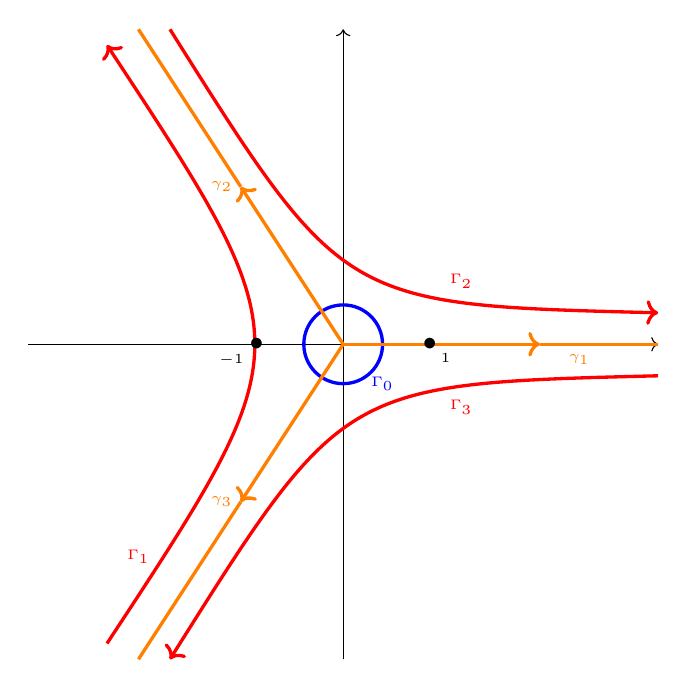
\begin{tikzpicture}
    \draw[->] (4,0)--(4,8);
    \draw[->] (0,4)--(8,4);
    \draw[blue,very thick] (4,4) circle (0.5) ;
    \node[blue,font=\tiny] at (4.5,3.5) {$\Gamma_0$};
    \node[red,font=\tiny] at (1.4,1.3) {$\Gamma_1$};
    \draw[red,very thick,->] (1,0.2) .. controls (3.5,4) .. (1,7.8);
    \node[red,font=\tiny] at (5.5,4.8) {$\Gamma_2$};
    \draw[red,very thick,->] (1.8,8) .. controls (4,4.5) ..(8,4.4) ;
     \node[red,font=\tiny] at (5.5,3.2) {$\Gamma_3$};
    \draw[red,very thick,->] (8,3.6) .. controls (4,3.5) ..(1.8,0) ;
    \draw[orange,very thick,->] (4,4)--(6.5,4);
    \draw[orange,very thick] (6.5,4)--(8,4);
    \node[orange,font=\tiny,below] at (7,4) {$\gamma_1$};
    \draw[orange,very thick,->] (4,4)--(2.7,6);
    \draw[orange,very thick] (2.7,6)--(1.4,8);
    \node[orange,font=\tiny,right] at (2.2,6) {$\gamma_2$};
    \draw[orange,very thick,->] (4,4)--(2.7,2);
    \draw[orange,very thick] (2.7,2)--(1.4,0);
    \node[orange,font=\tiny,right] at (2.2,2) {$\gamma_3$};
    \node at (5.1,4) {$\bullet$};
    \node at (2.9,4) {$\bullet$};
    \node[font=\tiny,below,right] at (2.3,3.8) {$-1$};
    \node[font=\tiny,below] at (5.3,4) {$1$};
    \end{tikzpicture}
    \caption{Representation of the path of integration for $A_k,B_0,B_k$ respectively in red, blue and orange.}\label{fig:path-generalized-Airy}
\end{figure}

Each generalized Airy function is a solution of

\begin{equation}
\left[\partial_z^3-z\partial_z+(p-1)\right]f(z,p)=0
\end{equation} 

and if $p=0$ they reduced to the classical Airy functions: $\mathrm{Ai}(z)=\mathrm{A}_1(z,0)$ and $\mathrm{Bi}(z)=\mathrm{B}_1(z,0)$.

We define the following exponential integral: let $p\geq 0$, $f(t)=4t^3-3t$ and $\nu_p=\tfrac{dt}{t^p}$. The critical points of $f$ are $\alpha_{\pm}:=\pm\tfrac{1}{2}$ (as for the classical Airy case), however the volume form $\nu_p$ is meromorphic    

\begin{equation}
I_\pm(z,p)\defeq\frac{1}{2\pi i}\int_{\Lambda_{\pm}}e^{-z(4t^3-3t)}\frac{dt}{t^p}
\end{equation}

where $\Lambda_{\pm}$ are the paths through the points $\alpha_\pm$, starting and ending at infinity (as in Figure \ref{fig:path-generalized-Airy-Lambda+-}).

\begin{figure}
\center
\begin{tikzpicture}
    \draw[->] (4,0)--(4,8);
    \draw[->] (0,4)--(8,4);
    \node[red,font=\tiny] at (1.4,1.3) {$\Lambda_-$};
    \draw[red,very thick,->] (1,0.2) .. controls (3.5,4) .. (1,7.8);
    %\node[red,font=\tiny] at (5.5,4.8) {$\Gamma_2$};
    %\draw[red,very thick,->] (1.8,8) .. controls (4,4.5) ..(8,4.4) ;
    % \node[red,font=\tiny] at (5.5,3.2) {$\Gamma_3$};
    %\draw[red,very thick,->] (8,3.6) .. controls (4,3.5) ..(1.8,0) ;
    \node[red,font=\tiny] at (7.4,1.3) {$\Lambda_+$};
    \draw[red,very thick,->] (7,0.2) .. controls (4.5,4) .. (7,7.8);
    \node at (5.1,4) {$\bullet$};
    \node at (2.9,4) {$\bullet$};
    \node[font=\tiny,below,right] at (2.3,3.8) {$-1$};
    \node[font=\tiny,below] at (5.3,4) {$1$};
    \end{tikzpicture}
    \caption{The paths of integration $\Lambda_\pm$ for $I_{\pm}$.}\label{fig:path-generalized-Airy-Lambda+-}
\end{figure}


In particular, $I_{+}(z,p)=(12 z)^{\tfrac{p-1}{3}}\mathrm{A}_1((\tfrac{3}{2}z)^{2/3},p)$: 

\begin{align*}
I_{+}(z,p)&=\frac{1}{2\pi i}\int_{\Lambda_{+}}e^{-z(4t^3-3t)}\frac{dt}{t^p} &\\
&=\frac{1}{2\pi i}(12 z)^{(p-1)/3}\int_{z^{-1/3}\Lambda_{+}}e^{-z(z^{-1}\frac{s^3}{3}-3 (12 z)^{-1/3}s)}\frac{ds}{s^p} & t=(12 z)^{-\tfrac{1}{3}}s\\
&=\frac{1}{2\pi i}(12 z)^{(p-1)/3}\int_{z^{-1/3}\Lambda_{+}}e^{-\left(\frac{s^3}{3}-(\tfrac{3}{2} z)^{2/3}s\right)}\frac{ds}{s^p} & \\
&=(12 z)^{(p-1)/3}\mathrm{A}_1((\tfrac{3}{2}z)^{2/3},p)
\end{align*}

It follows that $I_+(z)$ is a solution of


\begin{equation}\label{eq:I}
\left[\partial_z^3-\partial_z+\frac{2-p}{z}\partial_z^2+\frac{p-1}{z}+\frac{-1-3p+3p^2}{9}\frac{\partial_z}{z^2}+\frac{3+p-3p^2-p^3}{27z^3}\right]I_+(z,p)=0
\end{equation}

From the general theory of linear ODE, the formal integral solution of \eqref{eq:I} is a linear combination of three generators 
\begin{equation}
U_1z^{p-1}\tilde{W}_1(z)+U_2e^{-z}z^{-1/2}\tilde{W}_2(z)+U_3e^{z}z^{-1/2}\tilde{W}_3(z)
\end{equation}
 
where $\tilde{W}_1, \tilde{W}_2$ and $\tilde{W}_3$ are formal power seirs $\tilde{W}_{\mathbf{k}}(z)=\sum_{j\geq 0}a_{\mathbf{k},j}z^{-j}$, which are the unique (we fix $a_{k,0}=1$ for $k=1,2,3$) solution of 

\begin{multline}\label{w1}
\left[\partial_z^3-\partial_z-\frac{1-2p}{z}\partial_z^2+\frac{17-30p+12p^2}{9z^2}\partial_z+\frac{8}{27}\frac{p^3-6 p^2+ 11p- 6}{z^3}\right]\tilde{W}_1(z)=0
\end{multline}


\begin{multline}\label{w2}
\left[\partial_z^3-3\partial_z^2+2\partial_z+\frac{1-2p}{2z}\partial_z^2-\frac{1-2p}{z}\partial_z+\frac{5+24p+12p^2}{36z^2}\partial_z+\right.\\
\left.-\frac{5+24p+12p^2}{36z^2}-\frac{1}{z^3}\left(\frac{5}{24}+\frac{59}{108}p+\frac{5}{18}p^2+\frac{1}{27}p^3\right)\right]\tilde{W}_2(z)=0
\end{multline}

\begin{multline}\label{w3}
\left[\partial_z^3+3\partial_z^2+2\partial_z+\frac{1-2p}{2z}\partial_z^2+\frac{1-2p}{z}\partial_z+\frac{5+24p+12p^2}{36z^2}\partial_z+\right.\\
\left.+\frac{5+24p+12p^2}{36z^2}-\frac{1}{z^3}\left(\frac{5}{24}+\frac{59}{108}p+\frac{5}{18}p^2+\frac{1}{27}p^3\right)\right]\tilde{W}_3(z)=0
\end{multline}


Let us first study equation \eqref{w1}: its Borel transform is

\begin{multline*}
-\zeta^3\tilde{w}_1+\zeta\tilde{w}_1-(1-2p)\int_0^\zeta\tilde{w}_1(t)t^2dt+\frac{(17-30p+12p^2)}{9}\int_0^\zeta(-t\tilde{w}_1(t))(\zeta-t)dt+\\
+\frac{8}{27}(p^3-6p^2+11p-6)\int_0^\zeta\tilde{w}_1(t)\frac{(\zeta-t)^2}{2}dt=0
\end{multline*}

We differentiate three times, getting 

\begin{multline*}
\left(\zeta-\zeta^3\right)\tilde{w}_1^{(3)}(\zeta)+\left(3-2(5-p)\zeta^2\right)\tilde{w}_1''(\zeta)-\left(\frac{215}{9}-\frac{34}{3}p+\frac{4}{3}p^2\right)\zeta\tilde{w}_1'(\zeta)+\\
+\frac{8}{27}\left(p-\frac{9}{2}\right)\left(p-\frac{7}{2}\right)\left(p-\frac{5}{2}\right)\tilde{w}_1(\zeta)=0
\end{multline*}

we set $y=\zeta^2$

%\begin{multline}
%\left[-4y(y-1)(2y\partial_y^3+3\partial_y^2)+3(4y\partial_y^2+2\partial_y)-2(5-p)y(4y\partial_y^2+2\partial_y)+\right.\\
%\left.-2y\left(\frac{215}{9}-\frac{34}{3}p+\frac{4}{3}p^2\right)\partial_y+\frac{8}{27}\left(p-\frac{9}{2}\right)\left(p-\frac{7}{2}\right)\left(p-\frac{5}{2}\right)\right]\tilde{w}_1(y)=0
%\end{multline}
\begin{multline}\label{eq:hw1}
y^2(1-y)\tilde{w}_1^{(3)}(y)+y\left((p-\frac{13}{2})y+3\right)\tilde{w}_1''(y)-\left(y\left(\frac{305}{36}-\frac{10}{3}p+\frac{p^2}{3}\right)-\frac{3}{4}\right)\tilde{w}_1'(y)+\\
+\frac{1}{27}\left(p-\frac{5}{2}\right)\left(p-\frac{9}{2}\right)\left(p-\frac{7}{2}\right)\tilde{w}_1(y)=0
\end{multline}

which is a generalized hypergeomtric equation (~16.8.5 \cite{dlmf}) with parameters



\begin{align*}
\mathbf{a}_0=\left(\frac{3}{2}-\frac{p}{3};\frac{7}{6}-\frac{p}{3};\frac{5}{6}-\frac{p}{3}\right) & \qquad\qquad \mathbf{b}_0=\left(\frac{1}{2};\frac{3}{2}\right)
\end{align*}

therefore, $\tilde{w}_1(y)=c_1\,\,{}_3F_2\left(\mathbf{a}_0;\mathbf{b}_0;y\right)$. 

  

Then we look at equation \eqref{w2}: its Borel transform is

\begin{multline}
-\zeta^3\tilde{w}_2(\zeta)-3\zeta^2\tilde{w}_2(\zeta)-2\zeta\tilde{w}_2(\zeta)+\frac{1-2p}{2}\int_0^\zeta t^2\tilde{w}_2(t)dt-(1-2p)\int_0^\zeta(-t\tilde{w}_2(t))dt+\\
+\frac{5+24p+12p^2}{36}\int_0^\zeta(\zeta-t)(-t\tilde{w}_2(t))dt
-\frac{5+24p+12p^2}{36}\int_0^\zeta(\zeta-t)\tilde{w}_2(t)dt +\\
-\left(\frac{5}{54}+\frac{59}{108}p+\frac{5}{18}p^2+\frac{1}{27}p^3\right)\int_0^\zeta\frac{(\zeta-t)^2}{2}\tilde{w}_2(t)dt=0
\end{multline} 

and taking three derivatives it simplifies to 

\begin{multline}
\left[\left(\zeta^3+3\zeta^2+2\zeta\right)\partial_\zeta^3 +6\partial_\zeta^2+\left(p-\frac{17}{2}\right)\zeta\left(\zeta+\frac{1}{2}\right)\partial_\zeta^2+\right.\\
\left. \left(\frac{p^2}{3}+\frac{14}{3}p+\frac{581}{36}\right)\left(\zeta+1\right)\partial_\zeta+\frac{1}{27}\left(p+\frac{7}{2}\right)\left(p+\frac{11}{2}\right)\left(p+\frac{15}{2}\right)\right]\tilde{w}_2(\zeta)=0
\end{multline}

define $y=\zeta\left(\zeta+\frac{4}{3}\right)$

\begin{multline}\label{eq1}
\left[y\left(y+\frac{4}{9}\right)^2\partial_y^3+2\left(\frac{3}{2}y+\frac{4}{3}+\frac{y}{2}\left(\frac{17}{2}+p\right)\right)\left(y+\frac{4}{9}\right)\partial_y^2+\left(\frac{2}{3}+\frac{y}{4}\left(\frac{17}{2}+p\right)\right)\partial_y\right.\\
\left.+\frac{1}{4}\left(\frac{p^3}{3}+\frac{14}{3}p+\frac{581}{36}\right)\left(y+\frac{4}{9}\right)\partial_y+\frac{1}{8\cdot 27}\left(p+\frac{7}{2}\right)\left(p+\frac{11}{2}\right)\left(p+\frac{15}{2}\right)\right]\tilde{w}_2(y)=0
\end{multline}

which now looks like a generalized hypergeometric equation. Indeed setting $t=\tfrac{9}{4}y+1$, \eqref{eq1} reads

\begin{multline}
\left[t^2(1-t)\partial_t^3-t\left(\big(\frac{23}{4}+\frac{p}{2}\big)t-\frac{p}{2}-\frac{11}{4}\right)\partial_t^2-\left(-\frac{5}{8}-\frac{p}{4}+t\Big(\frac{887}{144}+\frac{17}{12}p+\frac{p^2}{12}\Big)\right)\partial_t +\right.\\
\left. -\frac{1}{8\cdot 27}\left(p+\frac{7}{2}\right)\left(p+\frac{11}{2}\right)\left(p+\frac{15}{2}\right)\right]\tilde{w}_2(t)=0
\end{multline}
hence a solution is given by the generalized hypergeometric function ${}_3F_2\left(\mathbf{a};\mathbf{b};y\right)$ with parameters

\begin{align*}
\mathbf{a}=\left(\frac{5}{4}+\frac{p}{6};\frac{7}{12}+\frac{p}{6};\frac{11}{12}+\frac{p}{6}\right) & \qquad\qquad \mathbf{b}=\left(\frac{1}{2};\frac{5}{4}+\frac{p}{2}\right)
\end{align*}

and we denote $\hat{w}_2(\zeta)=c_2\,\, {}_3F_2\left(\mathbf{a};\mathbf{b};\left(\tfrac{3}{2}\zeta+1\right)^2\right)$. The equation \eqref{w3} differs from \eqref{w2} for few signs: we find that its Borel transform is 

\begin{multline}
-\zeta^3\tilde{w}_2(\zeta)+2\zeta^2\tilde{w}_2(\zeta)-\frac{8}{9}\zeta\tilde{w}_2(\zeta)+\frac{1-2p}{2}\int_0^\zeta t^2\tilde{w}_2(t)dt+\frac{2-4p}{3}\int_0^\zeta(-t\tilde{w}_2(t))dt+\\
+\frac{5+24p+12p^2}{36}\int_0^\zeta(\zeta-t)(-t\tilde{w}_2(t))dt
+\frac{5+24p+12p^2}{54}\int_0^\zeta(\zeta-t)\tilde{w}_2(t)dt +\\
-\left(\frac{5}{54}+\frac{59}{108}p+\frac{5}{18}p^2+\frac{1}{27}p^3\right)\int_0^\zeta\frac{(\zeta-t)^2}{2}\tilde{w}_2(t)dt=0
\end{multline}

and differentiating three times we find a generalized hypergeometric equation with parameters $\mathbf{a},\mathbf{b}$ in the variable $y=\left(\tfrac{3}{2}\zeta-1\right)^2$, i.e. $\hat{w}_3(\zeta)= c_3\,\, {}_3F_2\left(\mathbf{a};\mathbf{b};\left(\tfrac{3}{2}\zeta-1\right)^2\right)$. In particular, 

\begin{equation}
\hat{w}_3(\zeta)=C_{23}\hat{w}_2(\zeta-\tfrac{4}{3})
\end{equation}

\textcolor{orange}{we may try to do the computations of Stokes constants for $p=1$, when $\hat{w}_1$ simplifies to a Gauss hypergeometric. Use also information about the monodromy. Check change of coordinates $y=\zeta^2$.}

\subsubsection{thimble projection formula}

In Theorem \ref{thm:maxim}, we proved a $3/2$-derivative formula to compute the Borel transform of the asymptotics of a thimble integral. 

\subsection{Third-order thimble integrals}

Let $f\colon\C\to \C$ be a degree three polynomial\footnote{Every degree three polynomial $a_3 u^3+a_2 u^2+a_1 u+a_0$ can be written in the form $a_3u^3+pu+q$, after a change of coordinates $u\to u-\frac{a_2}{3 a_3}$. Furthermore, we can restrict to monic polynomials by setting $a_3=1$.}, we are going to consider thimble integrals of the form 

\[ I_j(z) = \int_{\Lambda_j} \exp\left[z\big(u^3 + pu + q)\right]\,du \]

where $\Lambda_j$ is a thimble in $H_{1}^{B,z}$ through a critical point of $f$. We can distinguish between the case when $f$ has two distinct critical points $x_+, x_-$ and only one critical point $x$, which correspond respectively to the case $p\neq 0$ and $p=0$. \footnote{Equivalently, the difference between the generic case ($p\neq 0$) and the degenerate one ($p=0$) is visible from the ODE perspective as in the former case $I$ is a solution of degree two ODE \[\left[\partial_z^2 +2q \partial_z+\left(\frac{4p^3}{27}+q^2\right)+\frac{1}{z}\left(\partial_z +q \right)-\frac{1}{9z^2}\right]\Phi=0,\] while in the latter, $I$ solves a degree one ODE (see \eqref{eqn:degree-3-poly-1root}).}


Recall that translations and scaling-rotations act naturally on the image of $f\colon X\to \C$ ($f$ not necessarily a degree three polynomial), and their action transforms the thimble integral $I_j$ in the following ways:

\begin{itemize}
    \item \textbf{Action of translations:} let $q\in\C$, post-composing with translation of $q$ maps $f\to f+q$, thus 
    \begin{align*}
        \int_{\Lambda_j}e^{z (f+q)} \nu &= e^{qz} I_j(z)
    \end{align*}
    \item  \textbf{Action of scaling-rotations:} let $\gamma\in\C$, post-composing with scaling-rotations by $\gamma$ maps $f\to \gamma\cdot f$, thus 
    \begin{align*}
        \int_{\Lambda_j}e^{z (\gamma\cdot f)} \nu &= I_j(z \gamma)
    \end{align*}
\end{itemize}

In particular, we can always reduce to study the thimble integral in simpler situations. 

As an example, every degree three polynomial with distinct critical points can be transformed in the Chebyshev polynomial $T_3(t)=4 t^3-3t$, implying that the thimble integral $I_+$ can be transformed into the Airy--Lucas integral with parameter $m=1, n=3$. This follows by post-composing $f$ with a translation of $-q$ followed by a scaling-rotation of $\frac{ -i 3^{3/2}}{2 p^{3/2}}$

\begin{align*}
    f-q &= u^3 + pu \\
    (f-q) \cdot \frac{ -i 3^{3/2}}{2 p^{3/2}} &= 4 \Big(\sqrt{-\tfrac{3}{p}} \tfrac{u}{2} \Big)^{3} - 3\Big(\sqrt{-\tfrac{3}{p}} \tfrac{u}{2} \Big) \\
    &= 4 t^3- 3t 
\end{align*}

with $t= \sqrt{-\frac{3}{p}} \frac{u}{2}$. Then the thimble integral $I_+$ gets transformed into 

\begin{align*}
    e^{-zq} I_+\left(-\tfrac{i 3^{3/2}}{2 p^{3/2}} z\right)&= \int_{\Lambda_+} e^{z (4t^3-3t)} du\\
    &= 2\sqrt{-\tfrac{p}{3}} \int_{\Lambda_+} e^{z (4t^3-3t)} dt \\
    &= 2\sqrt{-\tfrac{p}{3}} K_{1/3}(z). 
\end{align*}

In particular, when $p\neq 0$, the thimble integral $I_+$ can be studied following the analysis of Appendix \ref{airy-appendix}. 
%In both cases, we will compute the differential equation satisfied by $I$. 

%\begin{lemma}
 %Let $f(u)=u^3+pu+q$, 
  %  \begin{itemize}
   %     \item if $p\neq 0$, then $I_{\pm}(z)$ solves 
    %    \begin{equation}\label{eqn:degree-3-poly-2roots}
    %        \left[\partial_z^2 +2q \partial_z+\left(\frac{4p^3}{27}+q^2\right)+\frac{1}{z}\left(\partial_z +q \right)-\frac{1}{9z^2}\right]\Phi=0
    %    \end{equation}
    %    \item  if $p=0$, then $I(z)$ solves
     %   \begin{equation}\label{eqn:degree-3-poly-1root}
      %      \left[\partial_z+q+\frac{1}{3z}\right]I=0
      %  \end{equation}
    %\end{itemize}
%\end{lemma}
%\begin{proof}
 %   The proof follows from a direct computation. 
%\end{proof}

%Let us first assume $p\neq 0$, then $x_{\pm}=\pm\sqrt{-p/3}$ and the critical values are $\alpha_{\pm}=f(x_\pm)$. Notice that equation \eqref{eqn:degree-3-poly-2roots} admits slight solutions as $\tau_\pm=\frac{1}{2}$ (recall the definition of $\tau\pm=\frac{Q(-\alpha_\pm)}{P'(-\alpha_\pm)}$ as in Section \ref{borel_reg-ODE}), thus, for $\theta=-\arg z$, $\laplace_{\zeta,f(\alpha_\pm)}^{\theta}v_\pm$ solves \eqref{eqn:degree-3-poly-2roots} if and only $v_\pm$ solves   

%\begin{equation}\label{eqn:deg3-borel-ODE}
 %   \left[\Big[\zeta^2-2q\zeta+\big(\frac{4p^3}{27}+q^2\big)\Big]\partial_\zeta^2+3(\zeta-q)\partial_\zeta+\frac{8}{9}\right]v_\pm=0
%\end{equation}

%Let us find a solution of \eqref{eqn:deg3-borel-ODE} slight at $\zeta=\alpha_+$: in the new coordinate $\zeta_+:=\zeta-\alpha_+$, equation \eqref{eqn:deg3-borel-ODE} becomes

%\begin{equation*}
 %   \left[\zeta_+ (\zeta_+ + \frac{4}{3}p\, x_+)\partial_{\zeta_+}^2+ \left[2p\, x_++3\zeta_{+}\right]\partial_{\zeta_+} +\frac{8}{9} \right]v_+=0
%\end{equation*}

%which is an hypergeometric equation in the coordinate $\xi=-\frac{3}{4p\,x_+}\zeta_+$

%\begin{equation*}
 %   \left[\xi (1-\xi)\partial_{\xi}^2+ 3\big(\frac{1}{2}-\xi\big)\partial_{\xi}-\frac{8}{9} \right]v_+=0
%\end{equation*}

%and it admits a slight solution \textcolor{red}{the solution should match with the one of airy, so choose $w_2$ in DLMf list and not $w_1$}

%\begin{align*}
 %   v_+ &= \xi^{-1/2}\, {}_2F_1\left(\frac{1}{6},\frac{5}{6} ;\frac{3}{2};1-\xi\right)\\
  %  &=\left(\frac{3}{4p\,x_+}\zeta_+\right)^{-1/2}\, {}_2F_1\left(\frac{1}{6},\frac{5}{6} ;\frac{3}{2};1-\frac{3}{4p\,x_+}\zeta_+\right). 
%\end{align*}

%Notice that $v_+$ is a hypergeometric function with the same parameters as the hypergeometric function $v_1$ in the example of Airy \S \ref{pos-root}. Similarly for $\zeta_-=\zeta-\alpha_-$ 

%\begin{equation*}
%    v_- =\left(\frac{3}{4p\,x_-}\zeta_-\right)^{-1/2}\, {}_2F_1\left(\frac{1}{6},\frac{5}{6} ;\frac{3}{2};1-\frac{3}{4p\,x_-}\zeta_-\right). 
%\end{equation*}


We then consider the case when $p=0$, and we study it both as a solution of an ODE and as a thimble integral.

First, notice that $I(z)$ solves
       \begin{equation}\label{eqn:degree-3-poly-1root}
          \left[\partial_z+q+\frac{1}{3z}\right]I=0
       \end{equation}

and we can find a Borel regular solution following the argument of \S \ref{big-idea}: $\laplace_{\zeta,\alpha}^{\theta}v$ is a solution of \eqref{eqn:degree-3-poly-1root} if and only if $v$ is a solution of 

\begin{align*}
   \left[ (\zeta-q)\partial_\zeta +\frac{2}{3}\right] v=0
\end{align*}

namely $v=(\zeta-q)^{-2/3}=\zeta_q^{-2/3}={}_2F_1\left(a,\frac{2}{3};a;1-\zeta_q\right)$, where $\zeta_q=\zeta-q$ and $a\in\C$ is a free parameter. 

The result is confirmed by the thimble projection reasoning which in this simple case reads

\begin{align*}
    \int_{\Lambda} e^{-z (u^3+q)} du &= e^{-zq} e^{i\pi/3} \int_0^{+e^{i\theta}\infty} e^{-z\zeta} \zeta^{-2/3} d\zeta\\
    &= e^{i\pi/3} \int_q^{+e^{i\theta}\infty} e^{-z\zeta} \, \zeta_q^{-2/3}\,  d\zeta
\end{align*}

where $e^{\pi i/3}$ accounts for the monodromy of $\zeta^{-2/3}$ at the origin. 


\color{DarkTurquoise}
\begin{itemize}
\item As $p$ goes to zero, $I(z)$ degenerates to
\[ \left(\tfrac{1}{2}\right)^{2/3} e^{-qz} \Gamma(\tfrac{1}{3}) z^{-1/3} = \left(\tfrac{1}{2}\right)^{2/3} e^{-qz} \laplace_{\zeta,0}(\zeta^{-2/3}) = \left(\tfrac{1}{2}\right)^{2/3} \laplace_{\zeta_{-q},q}(\zeta^{-2/3}). \]
\end{itemize}


\color{orange}
\section*{Outline}

\textbf{Title: Borel regularity and Resurgence of Exponential Integrals}

\begin{enumerate}
\item introduction
\begin{itemize}
\item Exponential integrals
\begin{itemize}
\item they are function of $z$ and they are defined from the data of $(X,f)$ and $[\mathcal{C}], [\nu]$
\item the choice of the path $\mathcal{C}$: 
\begin{itemize}
\item $\mathcal{C}\in H^{B,z}_{n}(X,f)$
\item Witten's formalism, $\mathcal{C}$ is a Lefschetz thimbles (or steepest descendent path)
\end{itemize}
\item they define a paring between the relative homology (rapid decaying homology)$H^{B,z}_{\bullet}(X,f)$ and the twisted de Rham cohomology  $H_{dR,z}^{\bullet}(X,f)$
\begin{itemize}
\item there is a comparison isomorphism (Maxim)
\end{itemize}
\item varying $z$ we have the Stokes phenomena
\item as $z\to\infty$, the asymptotic expansion of $I$ is a divergent series $\tilde{I}$, usually of Gevrey-class
\begin{itemize}
\item {\it exact resurgence relation} (Berry--Howls): divergence encodes contributions from other critical values
\item it is an example of resurgent series (\'Ecalle)
\item $\tilde{I}$ is resurgent in $\C\setminus\lbrace \text{poles of } \nu\,, \text{cirtical values of } f\rbrace$
\item it is a toy example of resurgent series because there are only finitely many singularities in the Borel plane
\item we have to compute the \textbf{Stokes constants} relative to the singular points in $B$ to fully understand $B$. There are two methods to compute Stokes constants: $\bullet$ geometric: using intersection theory of thimbles (Picard--Lefschtez, Witten, Maxim), $\bullet$ analytic: using \'Ecalle formalism   
\end{itemize} 
\end{itemize}
\item what are exponential integrals? \textcolor{gray}{has to be done}
\begin{itemize}
\item motivation
\begin{itemize}
\item In the classical theory of special functions, exponential integrals are often used to express solutions of linear differential and difference equations.
\item In physics ??
\item Geometrically they represent a Poincar\'e pairing (as explained by Kontsevich in \textbf{IHES lectures}).
\end{itemize}
\end{itemize}
\item What is the class of ODEs that we study? \textcolor{gray}{has to be done}
\item State results about resurgence of exponential integrals and Stokes phenomena
\begin{itemize}
\item Thimbles integrals [Kontsevich]: geometric computation of Stokes constants \textcolor{gray}{has to be done}
\item ODE and fractional derivative formula [{\tt draft2}]
\item if hypergeometric functions appear in a large class of examples: integral formulas for hypergeometric functions \textcolor{gray}{has to be done}
\end{itemize}
\end{itemize}
\item Formalism for Laplace transform [{\tt draft2}, ``The geometry of the Laplace transform'']
\begin{enumerate}
\item Analytic
\begin{enumerate}
\item Introduction
\item Brief revew of translation surfaces (we can refer to this from the introduction if we need to)
\item The Laplace transform of a holomorphic function
\begin{enumerate}
\item Over an ordinary point
\item Over a branch point
\item Differential equation
\end{enumerate}
\item Relating differential equations in the frequency domain to integral equations in the position domain
\end{enumerate}
\item Formal
\begin{enumerate}
\item Laplace transform of a formal series
\item Borel transform
\item Relating differential equations in the frequency variable to integral equations in the position variable
\end{enumerate}
\end{enumerate}
\item Review of integral equations
\begin{itemize}
\item Existence of solutions
\item Fractional integrals and derivatives
\item Going between integral and differential equations (slight functions)
\end{itemize}
\item General cases
\begin{enumerate}
\item Borel regularity
\begin{itemize}
\item General ODE of the form
\[ \left[ P\big(\tfrac{\partial}{\partial z}\big) + z^{-1} Q\big(\tfrac{\partial}{\partial z}\big) + z^{-2} R(z^{-1}) \right] \Phi = 0, \]
where $P$ is a polynomial, $Q$ is a polynomial of one degree lower, and $R$ is an entire function~\text[see {\tt airy-resurgence} and written notes]
\begin{itemize}
\color{DarkCyan}
\item More generally, for $P$ of degree $n$, we should be able to handle
\[ \left[ P\big(\tfrac{\partial}{\partial z}\big) + z^{-1} Q\big(\tfrac{\partial}{\partial z}\big) + z^{-2} R_2\big(\tfrac{\partial}{\partial z}\big) + \ldots + z^{-(n-1)} R_{n-1}\big(\tfrac{\partial}{\partial z}\big) + z^{-n} R(z^{-1}) \right] \Phi = 0, \]
where $R_k$ has degree $n-k$. \textcolor{gray}{has to be done}
\begin{itemize}
\item We want the most general ODE with a regular singularity at $z = 0$ and its only other singularity, typically irregular, at $z = \infty$. \textcolor{gray}{has to be done}
\item The singularity at $\infty$ should only be regular for an Euler equation. \textcolor{gray}{has to be done}
\end{itemize}
\color{orange}
\item Show that we can find a slight solution at each critical value.
\item Show that $\hat{\iota} = \tilde{\iota}$, where:
\begin{itemize}
\item $I = \laplace \iota$
\item $\hat{\iota}$ is the Taylor expansion of $\iota$
\item $\tilde{I}$ is the asymptotic series of $I$
\item $\tilde{\iota} = \borel \tilde{I}$
\item Idea: Show that $\hat{\iota}$ and $\tilde{\iota}$ have matching asymptotics at $\zeta = 0$. Since they both satisfy the position-domain integral equation, they must coincide.
\end{itemize}
\end{itemize}
\item General thimble integral (conditions?)
\begin{itemize}
\item Proof of Borel regularity
\item $3/2$-derivative formula
\item thimble projection reasoning
\end{itemize}
\end{itemize}
\item Resurgence
\begin{itemize}
\item Explain how Borel regularity relates resurgence of formal series to resurgence of holomorphic functions in the position domain. \textcolor{gray}{think more about what we're trying to say here}
\item Relate to Ecalle's formalism and the alien derivative
\item Stokes factors
\begin{itemize}
\item For ODEs
\item For thimble integrals
\end{itemize}
\end{itemize}
\end{enumerate}
\item Examples \textcolor{gray}{make sure each example contains a computation of the Borel transform, so we can see it matches}
\begin{enumerate}
\item The Airy example
\begin{itemize}
\item $I(z)$ is a solution of a linear ODE. We explicitly find its Borel transform, knowing the nature of singularities and the asymptotic behaviour of a basis of solution for the ODE  [{\tt airy-resurgence}]
\item Compute Stokes constants
\begin{itemize}
\item Using thimble projection formula and Borel transform computation [{\tt draft2}]
\item Using Picard-Lefschetz theory (Pham, Kontsevich, etc.)
\end{itemize}
\item Comparison with the literature \textcolor{gray}{has to be done}
\begin{itemize}
\item Mari\~{n}o
\item Sauzin
\item Kontsevich slides
\item Kawai--Takei? [might take too long to understand well enough]
\end{itemize}
\end{itemize}
\item The Airy--Lucas examples
\begin{itemize}
\item Compute Borel transform [{\tt airy-resurgence}]
\item Compute Stokes constants \textcolor{gray}{has to be done}
\end{itemize}
\item Bessel 0 (it is different because we have infinite cover)
\begin{itemize}
\item Compute Stokes constants [{\tt draft2}]
\end{itemize}
\item Bessel $\mu$ (follows from Bessel 0)
\begin{itemize}
\item Compute Stokes constants [{\tt modified Bessel}]
\end{itemize}
\item The generalized Airy example
\item The vibrating beam example
\begin{itemize}
\item In addition to the simple example, maybe we can do an example where the equation on the spatial domain includes fractional integrals since Andy is interested in that sort of thing
\end{itemize}
\end{enumerate}
\end{enumerate}

\color{black}

\appendix

\section{The Airy equation}\label{airy-appendix}

\subsubsection{Rewriting as a modified Bessel equation}
We can distill the most interesting part of the Airy function by writing
\[ \Ai(y) = \tfrac{1}{\pi\sqrt{3}}\,y^{1/2}\,K\big(\tfrac{2}{3} y^{3/2}\big), \]
where
\begin{equation}\label{integral:mod-bessel}
K(z) = i\sqrt{3} \int_{z^{-1/3}\Gamma} \exp\left[z \left(4u^3 - 3u\right)\right]\,du.
\end{equation}
Saying that $\Ai$ satisfies the Airy equation is equivalent to saying that $K$ satisfies the modified Bessel equation
\begin{equation}\label{eqn:mod-bessel-1/3}
\left[z^2 \big(\tfrac{\partial}{\partial z}\big)^2 + z \tfrac{\partial}{\partial z} - \big[\big(\tfrac{1}{3}\big)^2 + z^2\big]\right] K = 0.
\end{equation}
In fact, $K$ is the modified Bessel function $K_{1/3}$~\cite[equation~9.6.1]{dlmf}.

%The method we'll demonstrate in Section~\ref{spatial} works for any differential equation
%\[ \left[ P\big(\tfrac{\partial}{\partial z}\big) + z^{-1} Q\big(\tfrac{\partial}{\partial z}\big) + z^{-2} R(z^{-1}) \right] \varphi = 0, \]
%where $P$ is a polynomial, $Q$ is a polynomial of one degree lower, and $R$ is an entire function.
Like we did in equation~\eqref{eqn:reg-mod-bessel-AL}, we can rewrite the modified Bessel equation above as 

\begin{equation}\label{eqn:reg-mod-bessel}
\left[ \big[ \big(\tfrac{\partial}{\partial z}\big)^2 - 1 \big] + z^{-1} \tfrac{\partial}{\partial z} - \big(\tfrac{1}{3}\big)^2 z^{-2} \right] K = 0.
\end{equation}

\subsection{Asymptotic analysis}
From the general theory of ODE of Poincar\'e rank $1$, we know that the space of trans-series solutions of ~\eqref{eqn:reg-mod-bessel} has a basis of trans-monomials
\[ \{ e^{-\alpha z} z^{-\tau_\alpha}\,\series{W}_\alpha \mid \alpha^2 - 1 = 0 \} \]
where the $\series{W}_\alpha\in\C\llbracket z^{-1} \rrbracket$ are formal power series in $z^{-1}$. From equations 10.40.2 and 10.17.1 of \cite{dlmf}, we learn that $K \sim \left(\tfrac{\pi}{2}\right)^{1/2} e^{-z} z^{-1/2}\,\series{W}_1$, with
\begin{equation}\label{bessel-asymp}
\series{W}_1 = 1 - \frac{(\tfrac{1}{6})_1 (\tfrac{5}{6})_1}{2^1 \cdot 1!}\;z^{-1} + \frac{(\tfrac{1}{6})_2 (\tfrac{5}{6})_2}{2^2 \cdot 2!}\;z^{-2} - \frac{(\tfrac{1}{6})_3 (\tfrac{5}{6})_3}{2^3 \cdot 3!}\;z^{-3} + \ldots
\end{equation}

The holomorphic analysis in Section~\ref{spatial} will give us holomorphic solutions
\[ \{ e^{-\alpha z} z^{-\tau_\alpha}\,W_\alpha \mid \alpha^2 - 1 = 0 \}, \]
which seem analogous to the trans-monomials above. Borel summation makes the analogy precise. We will see in Section~\ref{bessel-regularity} that each $z^{-\tau_\alpha}\,W_\alpha$ is proportional to the Borel sum of $z^{-\tau_\alpha}\,\series{W}_\alpha$. This is an evidence of Theorem~\ref{thm1-dim}.

\subsection{Building a distinguished frame of analytic solutions}
\subsubsection{Going to the spatial domain}\label{spatial}
%\subsubsection{The big idea}\label{big-idea}
We are going to look for functions $v_\alpha$ whose Laplace transforms $\laplace_{\zeta, \alpha} v_\alpha$ satisfy equation~\eqref{eqn:reg-mod-bessel}. We will succeed when $\alpha^2 - 1 = 0$, and we will see that $K$ is a scalar multiple of $\laplace_{\zeta, 1} v_1$.

We can see from Section~\ref{L-int-op} that $\laplace_{\zeta, \alpha} v$ satisfies the differential equation~\eqref{eqn:reg-mod-bessel} if and only if $v$ satisfies the integral equation
\begin{equation}\label{int-eq:spatial-mod-bessel}
\left[ \big[ \zeta^2 - 1 \big] - \fracderiv{-1}{\zeta}{\alpha} \circ \zeta - \big(\tfrac{1}{3}\big)^2 \fracderiv{-2}{\zeta}{\alpha} \right] v = 0.
\end{equation}

It's tempting to differentiate both sides of this equation until we get
\begin{equation}\label{diff-eq:spatial-mod-bessel}
\left[ \big(\tfrac{\partial}{\partial \zeta}\big)^2 \circ \big[ \zeta^2 - 1 \big] - \tfrac{\partial}{\partial \zeta} \circ \zeta - \big(\tfrac{1}{3}\big)^2 \right] v = 0,
\end{equation}
which is easier to solve. However, as we learned in Section~\ref{shifting}, a solution of equation~\eqref{diff-eq:spatial-mod-bessel} satisfies equation~\eqref{int-eq:spatial-mod-bessel} if it's slight and locally integrable at $\zeta = \alpha$. 

This is great news, because equation~\eqref{diff-eq:spatial-mod-bessel} has a regular singularity at each root of $\zeta^2 - 1$, and the Frobenius method often gives a slight solution at each regular singular point. We can see the regular singularities by moving the derivatives to the right:
\[ \left[ (\zeta^2 - 1) \big(\tfrac{\partial}{\partial \zeta}\big)^2 + 3\zeta \tfrac{\partial}{\partial \zeta} + \big[ 1 - \big(\tfrac{1}{3}\big)^2 \big] \right] v = 0. \]

In Sections \ref{pos-root}\,--\,\ref{neg-root}, we will see this approach succeed. For each root $\alpha$, we'll find a solution $v_\alpha$ of equation~\eqref{diff-eq:spatial-mod-bessel} which is slight and locally integrable at $\zeta = \alpha$. We know the function $\laplace_{\zeta, \alpha} v_\alpha$ will satisfy equation~\eqref{eqn:reg-mod-bessel}, and we can even find its asymptotics from the order $\tau_\alpha$ of $v_\alpha$. We learned in Section~\ref{translation} that
\[ \laplace_{\zeta, \alpha} v_\alpha = e^{-\alpha z} V_\alpha \]
where $V_\alpha = \laplace_{\zeta_\alpha, 0} v_\alpha$ and $\zeta = \alpha + \zeta_\alpha$. We can see from Section~\ref{reg-decay} that $V_\alpha$ is asymptotic to a scalar multiple of $z^{ - \tau_\alpha}$ at $z = \infty$, so the further decomposition
\[ \laplace_{\zeta, \alpha} v_\alpha = e^{-\alpha z} z^{-\tau_\alpha} W_\alpha, \]
makes $W_\alpha$ is asymptotic to a scalar multiple of $1+O(z^{-1})$ at $z = \infty$.
%\textcolor{Magenta}{Show that $W_1$ is asymptotic to $\tilde{W}_1$!}
%\color{Peru}
%\begin{align*}
%\left[ \big(\tfrac{\partial}{\partial \zeta}\big)^2 \circ (\zeta - 1)(\zeta + 1) - \tfrac{\partial}{\partial \zeta} \circ \zeta - \big(\tfrac{1}{3}\big)^2 \right] v & = 0
%\end{align*}
%\color{Sienna}
%\begin{align*}
%\left[ \big[ 2 + 2(2\zeta) \tfrac{\partial}{\partial \zeta} + (\zeta^2 - 1) \big(\tfrac{\partial}{\partial \zeta}\big)^2 \big] - \big[ 1 + \zeta \tfrac{\partial}{\partial \zeta} \big] - \big(\tfrac{1}{3}\big)^2 \right] v & = 0 \\
%\left[ (\zeta^2 - 1) \big(\tfrac{\partial}{\partial \zeta}\big)^2 + 3\zeta \tfrac{\partial}{\partial \zeta} + \big[ 1 - \big(\tfrac{1}{3}\big)^2 \big] \right] v & = 0 \\
%\left[ (\zeta - 1)(\zeta + 1) \big(\tfrac{\partial}{\partial \zeta}\big)^2 + 3\zeta \tfrac{\partial}{\partial \zeta} + \big[ 1 - \big(\tfrac{1}{3}\big)^2 \big] \right] v & = 0
%\end{align*}
%\color{black}
%%In terms of the coordinate $\zeta_\alpha$ with $\zeta = \alpha + \zeta_\alpha$, this equation is written
%%\begin{equation}\label{eqn:centered-mod-bessel}
%%\[ \left[ \big[ \zeta_\alpha (\zeta_\alpha + 2\alpha) + \alpha^2 - 1 \big] + \fracderiv{-1}{\zeta_\alpha}{0} \circ \big[ \zeta_\alpha + \alpha \big] - \big(\tfrac{1}{3}\big)^2 \fracderiv{-2}{\zeta_\alpha}{0} \right] w = 0. \]
%%\end{equation}
\subsubsection{Focus on $\zeta = 1$}\label{pos-root}
Let's find a solution of equation~\eqref{diff-eq:spatial-mod-bessel} which is slight and locally integrable at $\zeta = 1$. Define a new coordinate $\zeta_1$ on $\C$ so that $\zeta = 1 + \zeta_1$. In this coordinate, equation~\eqref{diff-eq:spatial-mod-bessel} looks like
\begin{equation}%%\label{diff-eq:spatial-mod-bessel-pos}
\left[\zeta_1(2 + \zeta_1) \big(\tfrac{\partial}{\partial \zeta_1}\big)^2 + 3(1 + \zeta_1) \tfrac{\partial}{\partial \zeta_1} + \big[1 - \big(\tfrac{1}{3}\big)^2\big]\right] v = 0.
\end{equation}
With another change of coordinate, given by $\zeta_1 = -2\xi_1$, we can rewrite equation~\eqref{diff-eq:spatial-mod-bessel} as the hypergeometric equation
\begin{equation}\label{diff-eq:hypergeom-pos}
\left[\xi_1 (1 - \xi_1) \big(\tfrac{\partial}{\partial \xi_1}\big)^2 + 3(\tfrac{1}{2} - \xi_1) \tfrac{\partial}{\partial \xi_1} - \big[1 - \big(\tfrac{1}{3}\big)^2\big]\right] v = 0.
\end{equation}
Looking through the twenty-four expressions for Kummer's six solutions, we find one \cite[formula~15.10.12]{dlmf} which is manifestly slight and locally integrable at $\xi_1 = 0$:
\begin{alignat*}{2}
v_1 &=\;& \hphantom{-i\sqrt{2}}\,\xi_1^{-1/2} & {}_2F_1\big(\tfrac{1}{6}, \tfrac{5}{6}; \tfrac{1}{2}; \xi_1\big) \\
&=\;& -i\,\left(\frac{\zeta_1}{2}\right)^{-1/2} & {}_2F_1\big(\tfrac{1}{6}, \tfrac{5}{6}; \tfrac{1}{2}; -\tfrac{1}{2}\zeta_1\big)
\end{alignat*}
From the argument in Section~\ref{spatial}, we know that $\laplace_{\zeta, 1} v_1$ satisfies equation~\eqref{eqn:reg-mod-bessel}, and can be written as $e^{-z} V_1$, where $V_1 = \laplace_{\zeta_1, 0} v_1$. Since $v_1$ has order $-1/2$, the decomposition $V_1 = z^{1/2} W_1$ makes $W_1$ asymptotic to a scalar multiple of $z^{-1}$ at $z = \infty$.
\subsubsection{Focus on $\zeta = -1$}\label{neg-root}
Let's find a solution of equation~\eqref{diff-eq:spatial-mod-bessel} which is slight and locally integrable at $\zeta = -1$. In the rescaled coordinate from Section~\ref{pos-root}, this is the point $\xi_1 = 1$. Looking again through Kummer's table of solutions, we find another expression \cite[formula~15.10.14]{dlmf} which is manifestly slight and locally integrable at $\xi_1 = 1$:
\begin{alignat*}{2}
v_{-1} &=\;& (1-\xi_1)^{-1/2} & F\big(\tfrac{1}{6}, \tfrac{5}{6}; \tfrac{1}{2}; 1-\xi_1\big) \\
&=\;& \left(\frac{\zeta_{-1}}{2}\right)^{-1/2} & F\big(\tfrac{1}{6}, \tfrac{5}{6}; \tfrac{1}{2}; \tfrac{1}{2}\zeta_{-1}\big)
\end{alignat*}
where $\zeta_{-1}$ is the coordinate with $\zeta = -1 + \zeta_{-1}$. From the argument in Section~\ref{big-idea}, we know that $\laplace_{\zeta, -1} v_{-1}$ satisfies equation~\eqref{eqn:mod-bessel}, and can be written as $e^z V_{-1}$, where $V_{-1} = \laplace_{\zeta_{-1}, 0} v_{-1}$. Since $v_{-1}$, like our other solution, has order $-1/2$, the same decomposition $V_{-1} = z^{1/2} W_{-1}$ makes $W_{-1}$ asymptotic to a scalar multiple of $z^{-1}$ at $z = \infty$.

In this example, $v_1$ and $v_{-1}$ happen to be related by a symmetry: the M\"{o}bius transformation that pulls $\zeta$ back to $-\zeta$. Kummer's solutions typically come from six different hypergeometric equations, which are related by the M\"{o}bius transformations that permute their singularities. In our case, though, exchanging $1$ with $-1$ keeps equation~\eqref{diff-eq:spatial-mod-bessel} the same.

%\color{DodgerBlue}
%If we follow the routine from Section~\ref{pos-root}, rewriting equation~\eqref{diff-eq:spatial-mod-bessel} in the coordinate $\zeta_{-1}$ and then rewriting it again in a more recognizable form, we arrive at the hypergeometric equation
%\[ \left[\xi_{-1} (1 - \xi_{-1}) \big(\tfrac{\partial}{\partial \xi_{-1}}\big)^2 + 3(\tfrac{1}{2} - \xi_{-1}) \tfrac{\partial}{\partial \xi_{-1}} - \big[1 - \big(\tfrac{1}{3}\big)^2\big]\right] v = 0, \]
%where $\zeta_{-1} = 2\xi_{-1}$. This is the same as what we get by substituting $\xi_{-1}$ for $\xi_1$ in Section~\ref{pos-root}! In other words, the holomorphic map that pulls $\xi_{-1}$ back to $\xi_1$.
\subsection{Borel regularity}\label{bessel-regularity}
Recall that $\tilde{W}_1$ is a formal solution of \eqref{eqn:reg-mod-bessel}

\begin{equation}
\tilde{W}_1(z)=\sum_{n=0}^{\infty}\frac{\left(\frac{1}{6}\right)_n\left(\frac{5}{6}\right)_n}{n!}\frac{(-1)^n}{2^n}z^{-n}.
\end{equation}
Our goal is to prove that the Borel sum of $z^{-1/2}\tilde{W}_1$ is proportional to $V_1=\laplace_{\zeta_1,0}v_1$. 
%
%\subsubsection{Borel sum of $\tilde{W}_1$}
%
%Let us first compute the Borel transform of $\tilde{W}_1$:
%
%
%\begin{align*}
%\tilde{w}_1(\zeta)&=\delta+\sum_{n=1}^{\infty}\frac{\left(\frac{1}{6}\right)_n\left(\frac{5}{6}\right)_n}{n!}\frac{(-1)^n}{2^n}\frac{\zeta^{n-1}}{\Gamma(n)}\\
%&=\delta -\frac{1}{2}\sum_{n=0}^{\infty}\frac{\left(\frac{1}{6}\right)_{n+1}\left(\frac{5}{6}\right)_{n+1}}{\Gamma(n+2)n!}\frac{(-\zeta)^n}{2^n}\\
%&=\delta-\frac{1}{2}\frac{\Gamma(\frac{7}{6})\Gamma(\frac{11}{6})}{\Gamma(\frac{1}{6})\Gamma(\frac{5}{6})}\sum_{n=0}^{\infty}\frac{\left(\frac{7}{6}\right)_{n}\left(\frac{11}{6}\right)_{n}}{\Gamma(n+2)n!}\frac{(-\zeta)^n}{2^n}\\
%&=\delta-\frac{5}{72}\,\, {}_2F_1\left(\frac{7}{6},\frac{11}{6};2,-\frac{\zeta}{2}\right)
%\end{align*}

Let us compute the Borel transform of $z^{-1/2}\tilde{W}_1$: notice that the appropriate coordinate is $\zeta_1$ 

\begin{align*}
\borel\left[z^{-1/2}\tilde{W}_1(z)\right](\zeta_1)&=\borel\left[\sum_{n=0}^{\infty}\frac{\left(\frac{1}{6}\right)_n\left(\frac{5}{6}\right)_n}{n!}\frac{(-1)^n}{2^n}z^{-n-\frac{1}{2}} \right](\zeta_1)\\
&=\sum_{n=0}^{\infty}\frac{\left(\frac{1}{6}\right)_n\left(\frac{5}{6}\right)_n}{n!}\frac{(-1)^n}{2^n}\frac{\zeta_1^{n-\frac{1}{2}}}{\Gamma(n+\frac{1}{2})}\\
&=\zeta_1^{-1/2}\,\, {}_2F_1\left(\frac{1}{6},\frac{5}{6};\frac{1}{2};-\frac{\zeta_1}{2}\right)
\end{align*}

Comparing with the solution $v_1$ computed in Section~\ref{pos-root} we notice that \[v_1(\zeta_1)\propto \borel\left[z^{-1/2}\tilde{W}_1\right](\zeta_1)\]
therefore the Borel Laplace sum of $z^{-1/2}\tilde{W}_1$ is proportional to $V_1$. In particular, both $K$ and $e^{-z}V_1$ are analytic solutions of the Airy equation~\eqref{eqn:reg-mod-bessel} and they have the same asymptotics at $\infty$ up to a multiplicative constant. 

Similarly, if we consider the formal power series

\begin{equation}
\tilde{W}_{-1}(z)=\sum_{n=0}^{\infty}\frac{\left(\frac{1}{6}\right)_n\left(\frac{5}{6}\right)_n}{n!}\frac{1}{2^n}z^{-n}
\end{equation}

analogous computations give that $v_{-1}(\zeta_{-1})\propto\borel\left[z^{-1/2}\tilde{W}_{-1}\right](\zeta_{-1})$.

\subsection{thimble projection reasoning for the Airy function}\label{contour-argument}
Generalizing from Section~\ref{contour-argument-AL}, we can recast integral~\eqref{integral:mod-bessel} into the $\zeta$ plane by setting $-\zeta = 4u^3 - 3u$. Projecting $z^{-1/3} \Gamma$ to a contour $\gamma_z$ in the $\zeta$ plane and choosing the branch of $u$ that lifts $\gamma_z$ back to $z^{-1/3} \Gamma$, we have
\begin{equation}\label{integral:mod-bessel-zeta}
K = \frac{i}{\sqrt{3}} \int_{\gamma_z} e^{-z\zeta}\frac{d\zeta}{4u^2 - 1}.
\end{equation}
For $z \in (0, \infty)$, the contour $\gamma_z$ runs clockwise around $[1, \infty)$, as shown below. Let's assume $z \in (0, \infty)$ for the rest of the section. \textcolor{magenta}{[Our conclusions should probably hold whenever $\operatorname{Re}(z) > 0$.]}
\begin{center}
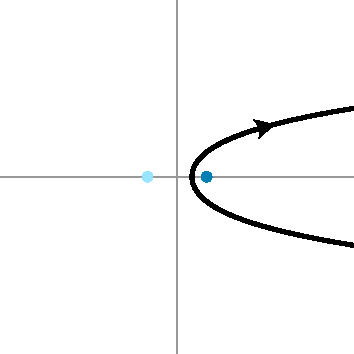
\includegraphics{figures/zeta_contour_3.pdf} \\[1em]
{\small The contour $\gamma_1$ in the $\zeta$ plane.}
\end{center}

From formula~15.4.14 in \cite{dlmf}, we learn that for our desired branch of $u$,
\[ \frac{1}{4u^2 - 1} = -F\big(\tfrac{1}{3}, \tfrac{2}{3}; \tfrac{1}{2}; \zeta^2\big), \]
so we can rewrite integral~\eqref{integral:mod-bessel-zeta} as
\[ K = \frac{1}{i\sqrt{3}} \int_{\gamma_z} e^{-z\zeta} F\big(\tfrac{1}{3}, \tfrac{2}{3}; \tfrac{1}{2}; \zeta^2\big)\;d\zeta. \]
This gives us an alternate route to the conclusion of Section~\ref{spatial}, which we'll follow below.

In addition to the solutions $v_1$ and $v_{-1}$ from Section~\ref{pos-root}\,--\, \ref{neg-root}, equation~\eqref{diff-eq:spatial-mod-bessel} has the solutions
\begin{alignat*}{2}
g_1 &\;=\;& & {}_2F_1\big(\tfrac{2}{3}, \tfrac{4}{3}; \tfrac{3}{2}; \xi_1\big) \\
g_{-1} &\;=\;&  & {}_2F_1\big(\tfrac{2}{3}, \tfrac{4}{3}; \tfrac{3}{2}; 1-\xi_1\big),
\end{alignat*}
given by formulas 15.10.11 and 15.10.13 from \cite{dlmf}.

The quadratic transformation identity 15.8.27 from \cite{dlmf} shows that\footnote{Note that $2\Gamma(\tfrac{1}{2})\Gamma(\tfrac{3}{2}) = 2\Gamma(\tfrac{1}{2})\,\tfrac{1}{2}\Gamma(\tfrac{1}{2}) = \pi$ and $\big[\Gamma(\tfrac{5}{6})\Gamma(\tfrac{7}{6})\big]^{-1} = \big[\Gamma(\tfrac{5}{6})\,\tfrac{1}{6}\Gamma(\tfrac{1}{6})\big]^{-1} = \frac{6\sin(\tfrac{1}{6} \pi)}{\pi} = \frac{3}{\pi}$.}
\[ F\big(\tfrac{1}{3}, \tfrac{2}{3}; \tfrac{1}{2}; \zeta^2\big) = \tfrac{1}{3}(g_1 + g_{-1}), \]
so we have
\[ K = \frac{1}{i\,3\sqrt{3}} \int_{\gamma_z} e^{-z\zeta} (g_1 + g_{-1})\;d\zeta. \]
The solution $g_{-1}$ is holomorphic on $\zeta \in [1, \infty)$, so it integrates to zero. The solution $g_1$, in contrast, is non-meromorphic at $\zeta = 1$. Along the branch cut $\zeta \in [1, \infty)$, its above-minus-below difference is $-\tfrac{3\sqrt{3}}{2}\,v_1$,
as given\footnote{Note that $\Gamma(\tfrac{3}{2}) \Gamma(\tfrac{1}{2})^{-1} = \tfrac{1}{2}$ and $\big[\Gamma(\tfrac{2}{3})\Gamma(\tfrac{4}{3})\big]^{-1} = \big[\Gamma(\tfrac{2}{3})\,\tfrac{1}{3}\Gamma(\tfrac{1}{3})\big]^{-1} = \frac{3\sin(\tfrac{1}{3} \pi)}{\pi} = \frac{3\sqrt{3}}{2\pi}$.} by equation~15.2.3 from \cite{dlmf}.
Hence,
\begin{align*}
K & = \frac{i}{2} \int^\infty_1 e^{-z\zeta} v_1\;d\zeta \\
e^z K & = \frac{i}{2} \int^\infty_1 e^{-z(\zeta - 1)} v_1\;d\zeta \\
e^z K & = \tfrac{i}{2} \laplace_{\zeta_1} v_1,
\end{align*}
just as we found in Section~\ref{bessel-regularity}.
\subsection{Another solution}
Section~\ref{contour-argument} associates the solution $K$ of equation~\eqref{eqn:mod-bessel} with the solution $g_1$ of equation~\eqref{diff-eq:hypergeom-pos}, which contributes the pole at $\zeta = 1$ of
\[ \frac{du}{d\zeta} = \frac{1}{4u^2 - 1} = \tfrac{1}{3}(g_1 + g_{-1}). \]
The solution $g_{-1}$, which contributes the pole at $\zeta = -1$, is associated with another solution of equation~\eqref{eqn:reg-mod-bessel}.

To express this other solution as a Laplace transform, following the method of Section~\ref{contour-argument}, we would use the solution
\[ v_{-1} = (1-\xi)^{-1/2} \,\, {}_2F_1\big(\tfrac{1}{6}, \tfrac{5}{6}; \tfrac{1}{2}; 1-\xi\big) \]
of equation~\eqref{diff-eq:spatial-mod-bessel}, given by formula~15.10.14 from \cite{dlmf}. This is the only solution, up to scale, which has a fractional power singularity at $\zeta = -1$.

In summary, the thimble projection technique of solving equation~\eqref{eqn:reg-mod-bessel} is associated with the basis
\begin{align*}
g_{1} & = {}_2F_1\big(\tfrac{2}{3}, \tfrac{4}{3}; \tfrac{3}{2}; \xi\big) \\
g_{-1} & = {}_2F_1\big(\tfrac{2}{3}, \tfrac{4}{3}; \tfrac{3}{2}; 1-\xi\big)
\end{align*}
of solutions for equation~\eqref{diff-eq:spatial-mod-bessel}, given by formulas 15.10.11 and 15.10.13 from \cite{dlmf}. These solutions contribute the poles at $\xi = 1$ and $\xi = 0$, respectively, of a generic solution.

The Laplace transformation method of solving equation~\eqref{eqn:reg-mod-bessel}, on the other hand, is associated with the basis
\begin{alignat*}{2}
v_{-1} &\;=\;& (1-\xi)^{-1/2} & \, {}_2F_1\big(\tfrac{1}{6}, \tfrac{5}{6}; \tfrac{1}{2}; 1-\xi\big) \\
v_1 &\;=\:& \xi^{-1/2} & \, {}_2F_1\big(\tfrac{1}{6}, \tfrac{5}{6}; \tfrac{1}{2}; \xi\big)
\end{alignat*}
given by formulas 15.10.14 and 15.10.12 from \cite{dlmf}. These solutions, up to scale, are the only ones with fractional power singularities.

Identities 15.10.18, and 15.10.22 from \cite{dlmf} give the change of basis
\begin{alignat*}{3}
v_{-1} &\;=\;&\tfrac{1}{\sqrt{3}}\,g_{-1} &\;+\;& \tfrac{1}{2}\,v_1 \\
v_1 &\;=\;& \tfrac{1}{\sqrt{3}}\,g_{1} &\;+\;& \tfrac{1}{2}\,v_{-1}.
\end{alignat*}
Summing these identities, we see that
\[ g_1 + g_{-1} = \tfrac{\sqrt{3}}{2}\,(f_1 + f_{-1}), \]
giving the alternate decomposition
\[ \frac{du}{d\zeta} = \tfrac{1}{2\sqrt{3}}\,(f_1 + f_{-1}). \]

\subsection{Thimble projection formula}

In an Airy-Lucas integral, $f$ is a Chebyshev polynomial, so we can do a thimble projection technique (\S \ref{contour-argument-AL}) or apply the thimble projection formula \eqref{formula1} \textcolor{red}{\footnote{We have this done in \texttt{draft2}, but we'll probably leave it out of the article}} using a trigonometric substitution. As an example of how one might reason in the latter case, we look at the Airy function ($f = 4u^3-3u$), this time using applying the thimble projection formula to the generalized Cardano's formula.

Recall that the roots of $f(u)-\zeta$ can be written explicitly as 

\begin{equation}
    u=????
\end{equation}


\subsection{Comparison with other treatments of the Airy equation}

\subsubsection{Different Borel transform convention} Physicists often use a different version of the Borel transform:
\begin{align*}
\borel_{\textit{phys}} \maps \C \llbracket z^{-1} \rrbracket & \to \C \llbracket \zeta \rrbracket \\
z^{-n} & \mapsto \frac{\zeta^n}{n!}.
\end{align*}
This version avoids sending $1$ to the convolution unit $\delta$, at the cost of no longer mapping multiplication to convolution or inverting the formal Laplace transform. It's sometimes convenient to $\borel_\textit{phys}(f) = \borel(z^{-1} f)$.

For problems involving a small parameter $\hbar$ rather than a large parameter $z$, physicists also define
\begin{align*}
\borel_{\textit{phys}} \maps \C \llbracket \hbar \rrbracket & \to \C \llbracket \zeta \rrbracket \\
\hbar^n & \mapsto \frac{\zeta^n}{n!}.
\end{align*}
From a combinatorial perspective, this is just the transformation that sends an ordinary generating function to the corresponding exponential generating function.

In \cite{lectures-Marino}, the author studies the Airy functions as an example of resurgent functions. He starts with the formal trans-monomial solutions of the Airy equation:

\begin{align*}
\tilde{\Phi}_{\mathrm{Ai}}(x)&=\frac{1}{2\sqrt{\pi}}x^{-1/4}e^{-\tfrac{2}{3}x^{3/2}}\tilde{W}_1(x^{-3/2})\\
\tilde{\Phi}_{\mathrm{Bi}}(x)&=\frac{1}{2\sqrt{\pi}}x^{-1/4}e^{\tfrac{2}{3}x^{3/2}}\tilde{W}_2(x^{-3/2})
\end{align*}  
where 
\begin{align*}
\tilde{W}_{1,2}(\hbar)=\sum_{n=0}^{\infty}\frac{1}{2\pi}\left(\mp\frac{3}{4}\right)^{n}\frac{\Gamma(n+\frac{5}{6})\Gamma(n+\frac{1}{6})}{n!}\hbar^n.
\end{align*}
%Notice that $\tilde{W}_{1,2}(\hbar)$ are proportional to $\tilde{W}_{\pm}(z)$ with $z=\hbar^{-1}$. However, their Borel transforms are two different hypergeometric functions:
Then, by applying the two definitions of the Borel transform $\borel_{\textit{phys}}$ and $\borel$, on the one hand we have  
\begin{align*}
w_{1,2}(\zeta)&\defeq\borel_{\textit{phys}}(\tilde{W}_{1,2})(\zeta)\\
&=\sum_{n=0}^{\infty}\frac{1}{2\pi}\left(\mp\frac{3}{4}\right)^{n}\frac{\Gamma(n+\frac{5}{6})\Gamma(n+\frac{1}{6})}{n!}\frac{\zeta^n}{n!}\\
&={}_2F_1\left(\frac{1}{6},\frac{5}{6};1;\mp\frac{3}{4}\zeta\right) 
\end{align*}
on the other hand, we find
\begin{align*}
\borel(\tilde{W}_{1,2})(\zeta)&=\frac{1}{2\pi}\delta+\sum_{n=1}^{\infty} \frac{1}{2\pi}\left(\mp\frac{3}{4}\right)^{n}\frac{\Gamma(n+\frac{5}{6})\Gamma(n+\frac{1}{6})}{n!}\frac{\zeta^{n-1}}{(n-1)!}\\
&=\frac{1}{2\pi}\delta+\sum_{n=0}^{\infty} \frac{1}{2\pi}\left(\mp\frac{3}{4}\right)^{n+1}\frac{\Gamma(n+1+\frac{5}{6})\Gamma(n+1+\frac{1}{6})}{(n+1)!}\frac{\zeta^{n}}{n!}\\
&=\frac{1}{2\pi}\delta\mp\frac{3}{4}\sum_{n=0}^{\infty} \frac{1}{2\pi}\left(\mp\frac{3}{4}\right)^{n}\frac{\Gamma(n+\frac{11}{6})\Gamma(n+\frac{7}{6})}{\Gamma(n+2)}\frac{\zeta^{n}}{n!}\\
&=\frac{1}{2\pi}\delta\mp\frac{5}{48} {}_2F_1\left(\frac{7}{6},\frac{11}{6};2;\mp\frac{3}{4}\zeta\right)%\\
%&=\frac{1}{2\pi}\delta\mp \frac{5}{48}\frac{1}{c_{1,2}}w_{\pm}(\zeta)
%w_{\pm}(\zeta)&=c_{1,2}\,\,{}_2F_1\left(\frac{7}{6},\frac{11}{6};2;\mp\frac{3}{4}\zeta\right) &\qquad \text{see \eqref{eq:hat+}\eqref{eq:hat-}}
\end{align*}
%That ambiguity comes from the different definitions of Borel transforms: 
%\begin{align*}
%\borel(\tilde{W}_{1,2})(\zeta)&=\frac{1}{2\pi}\delta+\sum_{n=1}^{\infty} \frac{1}{2\pi}\left(\mp\frac{3}{4}\right)^{n}\frac{\Gamma(n+\frac{5}{6})\Gamma(n+\frac{1}{6})}{n!}\frac{\zeta^{n-1}}{(n-1)!}\\
%&=\frac{1}{2\pi}\delta+\sum_{n=0}^{\infty} \frac{1}{2\pi}\left(\mp\frac{3}{4}\right)^{n+1}\frac{\Gamma(n+1+\frac{5}{6})\Gamma(n+1+\frac{1}{6})}{(n+1)!}\frac{\zeta^{n}}{n!}\\
%&=\frac{1}{2\pi}\delta\mp\frac{3}{4}\sum_{n=0}^{\infty} \frac{1}{2\pi}\left(\mp\frac{3}{4}\right)^{n}\frac{\Gamma(n+\frac{11}{6})\Gamma(n+\frac{7}{6})}{\Gamma(n+2)}\frac{\zeta^{n}}{n!}\\
%&=\frac{1}{2\pi}\delta\mp\frac{5}{48} {}_2F_1\left(\frac{7}{6},\frac{11}{6};2;\mp\frac{3}{4}\zeta\right)%\\
%%&=\frac{1}{2\pi}\delta\mp \frac{5}{48}\frac{1}{c_{1,2}}w_{\pm}(\zeta)
%\end{align*}  

and comparing the two solutions we notice that up to the factor of $\delta$

\begin{equation}\label{Borel-W12}
\borel(\tilde{W}_{1,2})(\zeta)-\frac{1}{2\pi}\delta=\mp \frac{5}{48} {}_2F_1\left(\frac{7}{6},\frac{11}{6};2;\mp\frac{3}{4}\zeta\right)=\frac{d}{d\zeta}\borel_{\textit{phys}}(\tilde{W}_{1,2})(\zeta) 
\end{equation}
More generally, if $\tilde{\Phi}(z)\in z^{-1}\C \llbracket z^{-1} \rrbracket$, i.e. it has no constant term, then 

\begin{equation}
\frac{d}{d\zeta}\circ\borel_{\textit{phys}}\tilde{\Phi}=\borel\tilde{\Phi}.
\end{equation}
In particular, $\frac{d}{d\zeta}\circ\borel_{\textit{phys}}\left[z^{-1/2}\tilde{W}_{1}\right]\left(\frac{2}{3}\zeta\right)=v_1(\zeta)$. 

%Recall that $v_1$ (computed in Section~\ref{pos-root}) is proportional to the Borel transform of $ z^{-1/2}\tilde{W}_1(z)$ (see Section~\ref{bessel-regularity}). We want to compare $v_1$ with the \textit{physic} Borel transform $\borel_{\textit{phys}}$ of $z^{-1/2}\tilde{W}_1$:
%
%\begin{align*}
%\borel_{\textit{phys}}(z^{-1/2}\tilde{W}_{1})\left(\frac{2}{3}\zeta\right)&=\sum_{n=0}^{\infty}\frac{1}{2\pi}\left(-\frac{1}{2}\right)^{n}\frac{\Gamma(n+\frac{5}{6})\Gamma(n+\frac{1}{6})}{n!}\frac{\zeta^{n+\frac{1}{2}}}{\Gamma(n+3/2)}\\
%&=\frac{1}{2\pi}\zeta^{-1/2}\sum_{n=0}^{\infty}\frac{\Gamma(n+\frac{5}{6})\Gamma(n+\frac{1}{6})}{n!\Gamma(n+3/2)}\left(-\frac{\zeta}{2}\right)^{n+1}\\
%&=\frac{1}{2\pi}\zeta^{1/2}\,\, {}_2F_1\left(\frac{1}{6},\frac{5}{6};\frac{3}{2};-\frac{\zeta}{2}\right) 
%\end{align*}
%
%Now taking the $-1$- derivative of $v_1(\zeta)$ we get
%
%\begin{align*}
%\partial_\zeta^{-1} v_1&=\frac{1}{\Gamma(1)}\int_0^{\zeta}(\zeta-\zeta') v_1(\zeta')d\zeta'\\
%&=\int_0^{\zeta}(\zeta-\zeta') \zeta'^{-1/2} \,\, {}_2F_1\left(\frac{1}{6},\frac{5}{6};\frac{1}{2};-\frac{\zeta'}{2}\right)d\zeta'\\
%&=\frac{\Gamma(1/2)}{\Gamma(3/2)}\zeta^{1/2} \,\, {}_2F_1\left(\frac{1}{6},\frac{5}{6};\frac{3}{2};-\frac{\zeta}{2}\right)\\
%&=2 \zeta^{1/2} \,\, {}_2F_1\left(\frac{1}{6},\frac{5}{6};\frac{3}{2};-\frac{\zeta}{2}\right)
%\end{align*}



\subsubsection{Integral formula for hypergeometric functions}

In \cite{diverg-resurg-i} the author studies summability and resurgent properties of solutions of the Airy equation. 

He considers the formal power series  
\[\tilde{\Phi}_{\pm}(z)\defeq \sum_{n=0}^{\infty}\frac{1}{2\pi}\left(\mp\frac{1}{2}\right)^{n}\frac{\Gamma(n+\frac{5}{6})\Gamma(n+\frac{1}{6})}{n!}z^{-n}\]
such that
\begin{align*}
\tilde{\Phi}_{\mathrm{Ai}}(y)&=\frac{1}{2\sqrt{\pi}}y^{-1/4}e^{-\tfrac{2}{3}y^{3/2}}\tilde{\Phi}_{+}\left(\tfrac{2}{3}y^{3/2}\right)\\
\tilde{\Phi}_{\mathrm{Bi}}(y)&=\frac{1}{2\sqrt{\pi}}y^{-1/4}e^{\tfrac{2}{3}y^{3/2}}\tilde{\Phi}_{-}\left(\tfrac{2}{3}y^{3/2}\right)
\end{align*} 
are formal solutions of the Airy equation. Notice that compared to Marino's formal solutions, Sauzin adopts a different change of coordinates $z=\frac{2}{3}y^{3/2}$.  

By looking for solutions of the Borel transformed equation, he wrote the Borel transform of $\tilde{\Phi}_{\pm}$ as a convolution product: 

\begin{align*}
\hat{\phi}_+(\zeta):=\borel\tilde{\Phi}_+=\delta+\frac{d}{d\zeta}\hat{\chi}(\zeta)  \qquad \hat{\phi}_-(\zeta):=\borel\tilde{\Phi}_-=\delta-\frac{d}{d\zeta}\hat{\chi}(-\zeta)
\end{align*}
 where $\hat{\chi}(\zeta)=\frac{2^{1/6}}{\Gamma(1/6)\Gamma(5/6)}(2\zeta+\zeta^2)^{-1/6}\ast \zeta^{-5/6}$.

%Notice that $\tilde{W}_{1,2}(\tfrac{2}{3}\hbar)=\tilde{\Phi}_{\pm}(z)$ for $\hbar=z^{-1}$, hence 
%
%\begin{align*}
%\tilde{\phi}_{+}(\zeta)&=\borel\tilde{W}_{1}(\tfrac{2}{3}\zeta)=\frac{1}{2\pi}\delta-\frac{5}{48} {}_2F_1\left(\frac{7}{6},\frac{11}{6};2;-\frac{\zeta}{2}\right) \\
%\tilde{\phi}_{-}(\zeta)&=\borel\tilde{W}_{2}(\tfrac{2}{3}\zeta)=\frac{1}{2\pi}\delta+\frac{5}{48} {}_2F_1\left(\frac{7}{6},\frac{11}{6};2;\frac{\zeta}{2}\right) 
%\end{align*}
%which up to a constant factor for $\delta$, they agree with our results. 

Notice that the function $\hat{\chi}(\zeta)$ is an hypergeometric function:

\begin{align*}
\hat{\chi}(\zeta)&=\frac{2^{1/6}}{\Gamma(1/6)\Gamma(5/6)}(2\zeta+\zeta^2)^{-1/6}\ast \zeta^{-5/6}\\
&=\frac{2^{1/6}}{\Gamma(1/6)\Gamma(5/6)}\int_0^{\zeta}(2\zeta'+\zeta'^2)^{-1/6} (\zeta-\zeta')^{-5/6}d\zeta'\\
&=\frac{2^{1/6}}{\Gamma(1/6)\Gamma(5/6)}\int_0^{1}(\zeta t)^{-1/6}(2+\zeta t)^{-1/6} (\zeta-\zeta t)^{-5/6} \zeta dt\\
&=\frac{2^{1/6}}{\Gamma(1/6)\Gamma(5/6)}\int_0^{1} t^{-1/6} 2^{-1/6}(1+\frac{\zeta}{2} t)^{-1/6} (1-t)^{-5/6}d\zeta'\\
&=\frac{1}{\Gamma(1/6)\Gamma(5/6)}\int_0^{1} t^{-1/6} (1+\frac{\zeta}{2} t)^{-1/6} (1-t)^{-5/6}d\zeta'\\
&={}_2F_1\left(\frac{1}{6},\frac{5}{6};1;-\frac{\zeta}{2}\right)
\end{align*}
where in the last step we use the Euler formula for hypergeometric functions \footnote{The Euler formula is \begin{equation}\label{Euler formula}
{}_{2}F_1\left(a,b;c;x\right)=\frac{\Gamma(c)}{\Gamma(b)\Gamma(c-b)}\int_0^1 t^{b-1}(1-t)^{c-b-1}(1-xt)^{-a}dt.
\end{equation}}. Then, by taking derivatives we recover $\hat{\phi}_{\pm}(\zeta)$: 

\begin{align*}
\hat{\phi}_+(\zeta)&=\delta-\frac{1}{2}\frac{5}{36}\,\, {}_2F_1\left(\frac{7}{6},\frac{11}{6};2;-\frac{\zeta}{2}\right)=\delta-\frac{2}{3}\frac{5}{48} {}_2F_1\left(\frac{7}{6},\frac{11}{6};2;-\frac{\zeta}{2}\right)\\
\hat{\phi}_-(\zeta)&=\delta+\frac{1}{2}\frac{5}{36}\,\, {}_2F_1\left(\frac{7}{6},\frac{11}{6};2;\frac{\zeta}{2}\right)=\delta+\frac{2}{3}\frac{5}{48} {}_2F_1\left(\frac{7}{6},\frac{11}{6};2;\frac{\zeta}{2}\right)
\end{align*} 
and up to a multiplicative constant they match our computations for $\borel(\tilde{W}_{1,2})$ (see equation~\eqref{Borel-W12}).
The main advantage of writing Gauss hypergeometric functions as a convolution product relies on Ecalle's singularity theory. Indeed $(2\zeta+\zeta^2)^{-1/6}$ extends analytically to the universal cover of $\C\setminus\lbrace 0,-2\rbrace$ and the convolution with $\zeta^{-5/6}$ does not change the set of singularities (see part c of \cite[Section 6.14.5]{diverg-resurg-i}). Furthermore, the author proves that $\hat{\phi}_{\pm}(\zeta)$ are simple resurgent functions (see \cite[Lemma 6.106]{diverg-resurg-i}). %Therefore, from the expression of $\chi(\zeta)$ as a convolution product, the resurgent properties of $\tilde{\phi}_{\pm}(\zeta)$ are evident.  

\subsubsection{Comparison with exact WKB}

Kawai and Takei study the WKB analysis of the Airy--type Schrodinger equation

\begin{equation}
\label{WKB_Airy} 
\left[\left(\frac{d}{dx}\right)^2 - \eta^2 x \right] \psi(x, \eta) = 0 
\end{equation}
as $\eta\to\infty$. They define $\psi_B(x, y)$ as the inverse Laplace transform of $\psi(x, \eta)$ with respect to $\eta$. In the coordinate $t=\frac{3}{2}yx^{-3/2}$ they find an explicit formula for $\psi_B(x,y)$ in terms of Gauss hypergeometric functions:
\begin{align*}
\psi_{+,B}(x,y)&=\frac{1}{x}\phi_+(t)=\frac{\sqrt{3}}{2\sqrt{\pi}}\frac{1}{x}s^{-1/2}\, {}_2F_1\left(\frac{1}{6},\frac{5}{6};\frac{1}{2};s\right)\\
\psi_{-,B}(x,y)&=\frac{1}{x}\phi_-(t)=\frac{\sqrt{3}}{2\sqrt{\pi}}\frac{1}{x}(1-s)^{-1/2}\, {}_2F_1\left(\frac{1}{6},\frac{5}{6};\frac{1}{2};1-s\right)
\end{align*}
where $s=t/2+1/2$. 
The same hypergeometric functions have been computed in Section \ref{Airy} as the Borel transform of the formal solutions of the Airy equation

\begin{equation}
\label{Airy}
\left[\left(\frac{d}{dw}\right)^2 -  w \right] f(w) = 0.
\end{equation}

Although the two equations look closely related (they are equivalent by the change of coordinates $w=x\eta^{2/3}$), the Borel transform of $\psi$ is computed with respect to $\frac{2}{3}\eta x^{3/2}$ (which is the conjugate variable of $t$) while the Borel transform of $f(w)$ is computed with respect to $w$. So we need to find a different change of coordinates to explain why the Borel transforms of $\psi(x,\eta)$ and $f(w)$ are given by the same hypergeometric function. 

First of all notice that if $\eta$ and $y$ are conjugate variables under Borel transform, meaning 
\begin{align*}
\sum_{n\geq 0}a_n\eta^{-n-1}  \overset{\borel}{\longrightarrow} \sum_{n\geq 0}\frac{a_n}{n!} y^{n} 
\end{align*} 
then $t=\frac{3}{2}yx^{-3/2}$ is the conjugate variable of $q=\frac{2}{3}\eta x^{3/2}$ up to correction by a factor of $\frac{3}{2}x^{-3/2}$
\begin{align*}
\sum_{n\geq 0}a_nq^{-n-1}=\sum_{n\geq 0}a_nx^{-3/2(n+1)}\left(\frac{2}{3}\eta\right)^{-n-1}  \overset{\borel}{\longrightarrow} \sum_{n\geq 0}\frac{a_nx^{-3/2(n+1)}}{n!}\left(\frac{3}{2}\right)^{n+1}  y^{n}=\frac{3}{2}x^{-3/2}\sum_{n\geq 0}\frac{a_n}{n!} t^{n}. 
\end{align*}
In addition, $\psi_{B,\pm}(x,y)=\frac{1}{x}\phi_{\pm}(t)$, therefore we expect that $\psi(x,\eta)=x^{1/2}\Phi(q)$. Assume that $\psi(x,y)$ is a solution of \eqref{WKB_Airy}, then $\Phi(q)$ solves 
\begin{equation}
\label{eq_Phi}
\left[\left(\frac{d}{dx}\right)^2+x^{-1}\frac{d}{dx}-\frac{1}{4}x^{-2} - \eta^2 x \right] \Phi(q) = 0
\end{equation}

\begin{proof}
\begin{align*}
&\left[\left(\frac{d}{dx}\right)^2 - \eta^2 x \right] \psi(x, \eta) = 0\\
&\left[\left(\frac{d}{dx}\right)^2 - \eta^2 x \right] x^{1/2}\Phi(q) = 0\\
&\frac{d}{dx}\left[\frac{1}{2}x^{-1/2}\Phi+x^{1/2}\frac{d}{dx}\Phi\right]-\eta^2x^{3/2}\Phi=0\\
&-\frac{1}{4}x^{-3/2}\Phi+\frac{1}{2}x^{-1/2}\frac{d}{dx}\Phi+\frac{1}{2}x^{-1/2}\frac{d}{dx}\Phi+x^{1/2}\left(\frac{d}{dx}\right)^2\Phi-\eta^2x^{3/2}\Phi=0\\
&\left[x^{1/2}\left(\frac{d}{dx}\right)^2+x^{-1/2}\frac{d}{dx}-\frac{1}{4}x^{-3/2}-\eta^2x^{3/2}\right]\Phi=0\\
&\left[\left(\frac{d}{dx}\right)^2+x^{-1}\frac{d}{dx}-\frac{1}{4}x^{-2}-\eta^2x\right]\Phi=0
\end{align*}
\end{proof}
Now rewrite \eqref{eq_Phi} in the coordinates $q=\frac{2}{3}\eta x^{3/2}$: 
\begin{align*}
&\left[\left(\frac{d}{dx}\right)^2+x^{-1}\frac{d}{dx}-\frac{1}{4}x^{-2}-\eta^2x\right]\Phi=0\\
&\left[\eta^2x\left(\frac{d}{dq}\right)^2+\frac{1}{2}\eta x^{-1/2}\frac{d}{dq}+x^{-1}\cdot\, \eta\,  x^{1/2}\frac{d}{dq}-\frac{1}{4}x^{-2}-\eta^2x\right]\Phi=0\\
&\left[\eta^2x\left(\frac{d}{dq}\right)^2+\frac{3}{2}\eta x^{-1/2}\frac{d}{dq}-\frac{1}{4}x^{-2}-\eta^2x\right]\Phi=0\\
&\left[\left(\frac{d}{dq}\right)^2+\frac{3}{2}\eta^{-1} x^{-3/2}\frac{d}{dq}-\frac{1}{4}\eta^{-2}x^{-3}-1\right]\Phi=0\\
%&\left[\left(\frac{d}{dq}\right)^2+\eta^{-1} x^{-3/2}\frac{d}{dq}-\frac{1}{9}\eta^{-2}x^{-3}-1\right]\Phi=0\\
&\left[\left(\frac{d}{dq}\right)^2+q^{-1}\frac{d}{dq}-\frac{1}{9}q^{-2}-1\right]\Phi=0
\end{align*}

therefore $\Phi(q)$ is a solution of the transformed Airy equation \eqref{eqn:reg-mod-bessel}. 

\begin{remark}
The change of coordinate $q=\frac{2}{3}\eta x^{3/2}$ is not casual: recall that the WKB ansatz for a Schrodinger type equation is

\begin{equation}
\psi(x,\eta)=\exp\left(\int_{x_0}^xS(\eta,x')dx'\right)
\end{equation} 
 and $S(\eta,x)=\sum_{k\geq -1}S_k(x)\eta^{-k}$. In addition, for the Airy--type Schrodinger equation 
 \begin{align*}
 S_{-1}^2=x
 \end{align*}
hence, up to a choice of sign for the square root
\begin{align*}
q&=\frac{2}{3}\eta x^{3/2}=\eta\int_0^x\sqrt{x'}dx'=\eta\int_{0}^xS_{-1}(x')dx'.
\end{align*}
We expect that the change of coordinates $q=\eta\int_0^{x}S_{-1}(x')dx'$ would explain the analogies between the Borel transform of the WKB solution of a Schrodinger equation and the Borel transform of the associated ODE.  
\end{remark} 

\section{Application of the integral formula}

In Section \ref{sec:examples}, we computed the Borel transform of the asymptotics of thimble integrals in different ways: on the one hand, using the thimble projection reasoning and on the other hand, solving an integral equation with a specified behavior near the singular point. In particular, we noticed that the two approaches give the same result up to the choice of a constant, as the integral equation is homogeneous. However, Theorem \ref{thm:maxim} suggests another approach, namely to use the fractional integral formula \eqref{formula1}. This approach  
As shown in the previous examples, the Borel transform  of the asymptotics of thimble integrals can be computed in different ways: from the ODE they solve, from the thimble projection reasoning, and from the integral formula \eqref{formula1}. When computed from the ODE, there is an ambiguity in the choice of a constant because the equation they satisfy is homogeneous, while with the thimble projection reasoning and the fractional integral formula the ambiguity is solved.

%In addition, since thimble integrals have a geometric interpretation, the Stokes constants that encode the jumps of thimble integrals when $z$ crosses a Stokes ray are expected to be integers as they are intersection numbers of dual pairs of thimbles. 

In Theorem \eqref{thm:maxim} we prove that the Borel transform of $\tilde{I}_{\alpha}$ can be computed by the thimble projection formula~\eqref{int:deriv-formula}. \color{olive} 

By general theory, it is expected that Stokes constants are integers, and numerically this can be verified only when a suitable normalization is chosen. Indeed as we have seen, if we consider exponential integrals the Borel transform can be computed in different ways: from the ODE, from the thimble projection reasoning, and from the integral formula. When computed from the ODE, there is an ambiguity in the choice of the constant, while with the thimble projection reasoning and the thimble projection formula the ambiguity is solved. We will see this for the modified Bessel equation. 

This method allows us to uniquely determine the constants $U_1,U_2$ that appear in the formal integral solution $\tilde{I}(z)$. Indeed, $\tilde{I}$ is a solution of an homogeneous linear ODE and $\tilde{I}_+(z)=U_1e^{-2/3z}z^{-1/2}\tilde{W}_+(z)$ for a particular choice of $U_1$. %In order to compute the Stokes constants we will first use the fractional derivative formula to compute the correct normalization of \[\hat{w}_\pm(\zeta)=\delta\mp \frac{5}{48}{}_2F_1\left(\frac{7}{6},\frac{11}{6};2;\mp\frac{3}{4}\zeta\right).\]   
\begin{lemma}\label{claim 2}
The following formula holds true
\[ \partial^{3/2}_{\zeta \text{ from } 2/3} \left( \int_{\mathcal{C}_+(\zeta)} \nu \right) = -i \frac{\sqrt{\pi}}{2}\,\hat{w}_+(\zeta-2/3), \]
for any $\zeta\in [2/3,+\infty)$.
\end{lemma}
\begin{proof}
In our general picture of exponential integrals, for $I_+(z)$ the thimble $\mathcal{C}_+$ is parametrized as the path $\theta \mapsto \cosh(\theta - \tfrac{2}{3}\pi i)$, $f = \tfrac{2}{3}(4u^3 - 3u)$ and $\nu = du$. Hence,
\begin{align*}
\int_{\mathcal{C}_+(\zeta)} \nu & = \int_{\mathcal{C}_+(\zeta)} du \\
& = u \Big|_{\operatorname{start} \mathcal{C}_+(\zeta)}^{\operatorname{end} \mathcal{C}_+(\zeta)}.
\end{align*}
Since $4u^3 - 3u$ is the third Chebyshev polynomial, and $\cosh$ is $2\pi$-periodic in the imaginary direction, the start and end points of $\mathcal{C}_+(\zeta)$ are characterized by
\begin{align*}
u & = \cosh(\mp\theta - \tfrac{2}{3}\pi i) \\
\zeta & = \tfrac{2}{3} \cosh(3\theta),
\end{align*}
so
\begin{align*}
\int_{\mathcal{C}_+(\zeta)} \nu & = \cosh(\theta - \tfrac{2}{3}\pi i) - \cosh(-\theta - \tfrac{2}{3}\pi i) \\
& = \big[\cosh(\theta) \cosh(-\tfrac{2}{3}\pi i) + \sinh(\theta) \sinh(-\tfrac{2}{3}\pi i)\big] \\
& \quad - \big[\cosh(-\theta) \cosh(-\tfrac{2}{3}\pi i) + \sinh(-\theta) \sinh(-\tfrac{2}{3}\pi i)\big] \\
& = 2\sinh(\theta) \sinh(-\tfrac{2}{3}\pi i) \\
& = -i\sqrt{3}\,\sinh(\theta)
\end{align*}
with $\tfrac{3}{2} \zeta = \cosh(3\theta)$. Let $\xi = \tfrac{1}{2}(1 - \tfrac{3}{2}\zeta)$, and notice that $\xi = -\sinh(\tfrac{3}{2} \theta)^2$ at the start and end points. The identity~15.4.16 \cite{dlmf}
\[ \sinh(\theta) = \tfrac{2}{3} \sinh(\tfrac{3}{2} \theta)\,{}_2F_1\big(\tfrac{1}{6}, \tfrac{5}{6}; \tfrac{3}{2}; -\sinh(\tfrac{3}{2} \theta)^2\big) \]
then shows us that
\[ \frac{i}{\sqrt{3}} \int_{\mathcal{C}_+(\zeta)} \nu = \tfrac{2}{3} (-\xi)^{1/2}\,{}_2F_1\big(\tfrac{1}{6}, \tfrac{5}{6}; \tfrac{3}{2}; \xi\big). \]

Now we can evaluate the half-integral of $\int_{\mathcal{C}_+} \nu$ using Bateman's fractional integral formula for hypergeometric functions see \S 4.1 in \cite{koornwinder2015fractional}.
\begin{align*}
\partial^{-1/2}_{\zeta \text{ from } 2/3} \left( \int_{\mathcal{C}_+(\zeta)} \nu \right) & = \frac{1}{\Gamma\big(\tfrac{1}{2}\big)} \int_{2/3}^\zeta (\zeta - \zeta')^{-1/2} \left( \int_{\mathcal{C}_+(\zeta')} \nu \right)\,d\zeta' \\
& = \frac{1}{\Gamma\big(\tfrac{1}{2}\big)} \int_0^\xi \tfrac{\sqrt{3}}{2} (\xi' - \xi)^{-1/2} \Big[ -{i}{\sqrt{3}}\,\tfrac{2}{3} (-\xi)^{1/2}\,{}_2F_1\big(\tfrac{1}{6}, \tfrac{5}{6}; \tfrac{3}{2}; \xi\big) \Big] \,\big( -\tfrac{4}{3}\,d\xi' \big) \\
& = -i \frac{4}{3} \frac{\Gamma\big(\tfrac{3}{2}\big)}{\Gamma(2)} (-\xi)\,{}_2F_1\big(\tfrac{1}{6}, \tfrac{5}{6}; 2; \xi\big) \\
& = i \frac{2}{3} \sqrt{\pi}\,\xi\, {}_2F_1\big(\tfrac{1}{6}, \tfrac{5}{6}; 2; \xi\big).
\end{align*}
Finally, we differentiate twice using 15.5.4 and 15.5.1 from \cite{dlmf}.
\begin{align*}
\partial^{3/2}_{\zeta \text{ from } 2/3} \left( \int_{\mathcal{C}_+(\zeta)} \nu \right) & = \left(-\tfrac{3}{4} \tfrac{\partial}{\partial \xi}\right)^2 \left[ i \frac{2}{3} \sqrt{\pi}\,\xi\, {}_2F_1\big(\tfrac{1}{6}, \tfrac{5}{6}; 2; \xi\big) \right] \\
& = i \tfrac{3\sqrt{\pi}}{8} \left(\tfrac{\partial}{\partial \xi}\right)^2 \left[ \xi\,{}_2F_1\big(\tfrac{1}{6}, \tfrac{5}{6}; 2; \xi\big) \right] \\
& = i \tfrac{3\sqrt{\pi}}{8}\,\tfrac{\partial}{\partial \xi} \left[ {}_2F_1\big(\tfrac{1}{6}, \tfrac{5}{6}; 1; \xi\big) \right] \\
& = i \tfrac{\sqrt{\pi}}{8}\,\tfrac{5}{12}\, {}_2F_1\big(\tfrac{7}{6}, \tfrac{11}{6}; 2; \xi\big).
\end{align*}
\end{proof}
Analogously, we can compute the correct constants for $\hat{w}_-(\zeta)$:

\begin{lemma}\label{claim 3}
For any $\zeta\in (-\infty,-2/3]$
\[ \partial^{3/2}_{\zeta \text{ from } -2/3} \left( \int_{\mathcal{C}_-(\zeta)} \nu \right) = - \frac{\sqrt{\pi}}{2}\,\hat{w}_-(\zeta+2/3). \]
\end{lemma}
\begin{proof}
Let $\mathcal{C}_-$ is the path $\theta \mapsto -\cosh(\theta - \tfrac{2}{3}\pi i)$, when $x \in [0, \infty)$ 
\[ I_-(z) = \int_{\mathcal{C}_-} \exp\left[-\tfrac{2}{3} z \left(4u^3 - 3u\right)\right]\,du. \]
In our general picture of exponential integrals, $f = \tfrac{2}{3}(4u^3 - 3u)$ and $\nu = du$. Hence,
\begin{align*}
\int_{\mathcal{C}_-(\zeta)} \nu & = \int_{\mathcal{C}_-(\zeta)} du \\
& = u \Big|_{\operatorname{start} \mathcal{C}_-(\zeta)}^{\operatorname{end} \mathcal{C}_-(\zeta)}.
\end{align*}
The start and end points of $\mathcal{C}_-(\zeta)$ are characterized by
\begin{align*}
u & = -\cosh(\mp\theta - \tfrac{2}{3}\pi i) \\
\zeta & = -\tfrac{2}{3} \cosh(3\theta),
\end{align*}
so
\begin{align*}
\int_{\mathcal{C}_-(\zeta)} \nu & =- \cosh(\theta - \tfrac{2}{3}\pi i) + \cosh(-\theta - \tfrac{2}{3}\pi i) \\
& =- \big[\cosh(\theta) \cosh(-\tfrac{2}{3}\pi i) + \sinh(\theta) \sinh(-\tfrac{2}{3}\pi i)\big] \\
& \quad + \big[\cosh(-\theta) \cosh(-\tfrac{2}{3}\pi i) + \sinh(-\theta) \sinh(-\tfrac{2}{3}\pi i)\big] \\
& = 2\sinh(\theta) \sinh(\tfrac{2}{3}\pi i) \\
& = i\sqrt{3}\,\sinh(\theta)
\end{align*}
with $\tfrac{3}{2} \zeta = -\cosh(3\theta)$. Let $\xi = \tfrac{1}{2}(1 + \tfrac{3}{2}\zeta)$, and notice that $\xi =- \sinh(\tfrac{3}{2} \theta)^2$ at the start and end points. The identity~15.4.16 in \cite{dlmf}
\[ \sinh(\theta) = \tfrac{2}{3} \sinh(\tfrac{3}{2} \theta)\, {}_2F_1\big(\tfrac{1}{6}, \tfrac{5}{6}; \tfrac{3}{2}; -\sinh(\tfrac{3}{2} \theta)^2\big) \]
then shows us that
\[ -\frac{i}{\sqrt{3}} \int_{\mathcal{C}_-(\zeta)} \nu = \tfrac{2}{3} (-\xi)^{1/2}\, {}_2F_1\big(\tfrac{1}{6}, \tfrac{5}{6}; \tfrac{3}{2}; \xi\big). \]

Now we can evaluate the half-integral of $\int_{\mathcal{C}_-} \nu$ using Bateman's fractional integral formula for hypergeometric functions (see \S 4.1 in \cite{koornwinder2015fractional}).
\begin{align*}
\partial^{-1/2}_{\zeta \text{ from } -2/3} \left( \int_{\mathcal{C}_-(\zeta)} \nu \right) & = \frac{1}{\Gamma\big(\tfrac{1}{2}\big)} \int_{-2/3}^\zeta (\zeta - \zeta')^{-1/2} \left( \int_{\mathcal{C}_-(\zeta')} \nu \right)\,d\zeta' \\
& = \frac{1}{\Gamma\big(\tfrac{1}{2}\big)} \int_0^\xi \tfrac{\sqrt{3}}{2} (\xi - \xi')^{-1/2} \Big[{i}{\sqrt{3}}\,\tfrac{2}{3} (-\xi')^{1/2}\, {}_2F_1\big(\tfrac{1}{6}, \tfrac{5}{6}; \tfrac{3}{2}; \xi' \big) \Big] \,\big( \tfrac{4}{3}\,d\xi' \big) \\
& =  \frac{4}{3} \frac{\Gamma\big(\tfrac{3}{2}\big)}{\Gamma(2)} (-\xi)\, {}_2F_1\big(\tfrac{1}{6}, \tfrac{5}{6}; 2; \xi\big) \\
& = - \frac{2}{3} \sqrt{\pi}\,\xi\,{}_2F_1\big(\tfrac{1}{6}, \tfrac{5}{6}; 2; \xi\big).
\end{align*}
Finally, we differentiate twice using 15.5.4 and 15.5.1 from \cite{dlmf}
\begin{align*}
\partial^{3/2}_{\zeta \text{ from } 2/3} \left( \int_{\mathcal{C}_+(\zeta)} \nu \right) & = \left(\tfrac{3}{4} \tfrac{\partial}{\partial \xi}\right)^2 \left[ - \frac{2}{3} \sqrt{\pi}\,\xi\, {}_2F_1\big(\tfrac{1}{6}, \tfrac{5}{6}; 2; \xi\big) \right] \\
& = - \tfrac{3\sqrt{\pi}}{8} \left(\tfrac{\partial}{\partial \xi}\right)^2 \left[ \xi\, {}_2F_1\big(\tfrac{1}{6}, \tfrac{5}{6}; 2; \xi\big) \right] \\
& = - \tfrac{3\sqrt{\pi}}{8}\,\tfrac{\partial}{\partial \xi} \left[ {}_2F_1\big(\tfrac{1}{6}, \tfrac{5}{6}; 1; \xi\big) \right] \\
& = - \tfrac{\sqrt{\pi}}{8}\,\tfrac{5}{12}\, {}_2F_1\big(\tfrac{7}{6}, \tfrac{11}{6}; 2; \xi\big).
\end{align*}
\end{proof}

\color{black}

\bibliographystyle{plain}
\bibliography{airy-resurgence}

\end{document}